% !TeX spellcheck = en_US
\chapter{Methodology}%
\label{method}


\section{Framework Architecture}

%To address the derived challenges and develop the required features from Section~\ref{summary_relatedwork}, we definethe following requirements which are crucial for developing modeling frameworks used for synthesis of E/E architectures and systems.


    In order to tackle the difficulties and overcome the obstacles and limitations identified in Section~\ref{summary_relatedwork} and answering the defined research questions in Chapter~\ref{intro}, it is essential to establish a set of requirements that can guide the development of modeling frameworks used for the synthesis of E/E architectures and systems.

\begin{itemize}
    \item Easing E/E architecture design: %To design E/E systems and vehicle network topology which comprise various hardware/software components and properties, different safety requirements, etc, graphical and textual modeling elements are needed. By having these modeling elements, the E/E architectures/systems can be easily modeled using drag\&drop feature.  
    various hardware/software components, safety requirements, and other properties need to be taken into consideration when designing E/E systems and vehicle network topology. To accomplish this, graphical and textual modeling elements are necessary. These modeling elements enable E/E architectures/systems to be easily modeled using drag and drop features. This feature allows designers to create and manipulate components with ease and flexibility. Furthermore, the drag and drop feature makes it easy to create and edit models, thus reducing the time and effort required to design an E/E architecture.
    
    
    %To design an E/E system or vehicle network topology, it's essential to consider various factors such as the hardware and software components, different safety requirements, and other important properties. For instance, the architecture of a modern vehicle comprises various electronic components, such as advanced driver-assistance systems (ADAS), infotainment systems, powertrain control modules, and more. Therefore, designing a complex E/E architecture system that integrates these components requires sophisticated modeling tools.In recent years, graphical and textual modeling elements have become popular in the automotive industry as they enable designers to create detailed models of the E/E architecture. These modeling elements offer a wide range of benefits, such as ease of use, accuracy, and flexibility, making it possible to design complex systems with ease.One of the significant advantages of using graphical and textual modeling elements is the ability to model E/E architectures and systems using drag and drop features. This feature allows designers to create and manipulate components with ease and flexibility. Furthermore, the drag and drop feature makes it easy to create and edit models, thus reducing the time and effort required to design an E/E architecture.Overall, the use of graphical and textual modeling elements has revolutionized the way E/E architecture is designed. It has enabled designers to create detailed models of E/E systems and vehicle network topology, which are essential for building safe and reliable vehicles.
    
    
    
    \item Flexibility and adaptability: The modeling framework should be flexible enough to accommodate various design requirements, and adaptable to changes in the system's specifications or design goals.
    
    \item Scalability: The framework should be scalable to handle systems of different sizes and complexities, from simple components to large-scale systems.
    
    \item Quick access to components, elements, and properties: %After an E/E architecture is modeled, an approach is required to provide an easy access to the modeling elements and their properties. In other words, this approach decreases the programming efforts for each specific design. 
    In the field of automotive engineering, designing an E/E system or car network topology involves creating a complex architecture that includes a wide range of interconnected components, elements, and properties. Once this architecture has been modeled, it is essential to have a way to quickly and easily access all of these elements and their associated properties.
    By having quick access to these elements and properties, designers/system integrators can streamline their programming efforts and avoid the time-consuming process of manually coding each component and property. This approach also allows for easier modification and testing of the system, as designers can quickly make changes to specific elements and properties without having to rewrite large portions of code.

%To facilitate this type of quick access, there are various tools and software solutions available that allow designers to easily navigate and modify the E/E system or car network topology. These tools often include features such as drag-and-drop interfaces, searchable element libraries, and customizable templates, making it easier for designers to quickly access and modify the various components of their design.

%Overall, having a streamlined approach to accessing the elements and properties of an E/E system or car network topology is essential for efficient and effective design. By using the right tools and software solutions, designers can significantly reduce their programming efforts and create more robust, reliable systems.
    
    \item Facilitating E/E architecture synthesis: %To reduce the synthesis complexity of E/E systems, methods are required to automate mapping, communication message routing, and scheduling by solving a constraint-based system model. In addition, all safety requirements can be transformed into constraints and then solved which have a significant impact on decrease of time and complexity.  
    As vehicles continue to become more complex and require more computational power, there is a growing need for efficient methods to automate the process of mapping, communication message routing, and scheduling.
    To achieve this, constraint-based system models can be employed. These models can automate the mapping and scheduling for E/E systems including multi-core architectures, and can also transform safety requirements into constraints that can be easily solved and utilized for E/E configurations. This not only reduces the complexity of the process, but also significantly decreases the time required for synthesis. In addition to these benefits, facilitating E/E architecture synthesis can also lead to improved vehicle safety and reliability. By automating the process, errors and inconsistencies can be minimized, ensuring that the resulting E/E systems fulfill all safety requirements and operate as intended.
    
    
    
    %Facilitating the synthesis of Electrical/Electronic (E/E) architecture is becoming increasingly important in the modern automotive industry. 
    


    
    \item Optimization: %System integrators should be allowed to optimize their designed E/E systems based on the different criteria and objectives. The optimization goals can include cost, redundancy, timing, reliability, etc.
    It is a critical consideration for any E/E system design, and system integrators should be given the freedom to optimize their designs based on various criteria and objectives. One of the most significant factors in optimization is cost, as the cost of an E/E system can be a determining factor in whether a project is feasible or not. By allowing system integrators to optimize their designs based on cost, they can create efficient and cost-effective solutions that meet the required performance and reliability standards while keeping the project within budget.
    In addition to cost, redundancy, reliability, FFI, timing, etc.  
    
    %is another critical optimization factor that system integrators must consider. 
%Redundancy is the inclusion of backup systems that can take over if the primary system fails. By incorporating redundancy into E/E system designs, system integrators can ensure that the system can continue to function even in the event of a failure, thus reducing the risk of downtime or system failure.

%Timing is also a crucial factor in E/E system optimization, particularly in systems that require real-time performance, such as those used in industrial control or transportation systems. By optimizing the design for timing, system integrators can ensure that the system can operate within the required response times and meet critical deadlines, such as in time-critical applications like air traffic control or autonomous vehicles.

%Reliability is another essential optimization goal that system integrators should consider. A reliable E/E system is one that can perform its intended function without failure, even in demanding or harsh environments. By optimizing the design for reliability, system integrators can incorporate features such as fault-tolerant systems, component redundancy, and predictive maintenance, which can improve the overall reliability of the system and reduce the risk of downtime or system failure.
    
    
    
    \item Synthesis time: %the solving time is a critical parameter to reduce E/E configuration effort and time. An approach should be considered to speed up the solving process which can be a single-step solving. This avoids multiple iterations to clarify a solution using design space exploration technique and also respect interrelations between specified constraints decisions.  
     %solving time is a critical parameter for reducing E/E configuration effort and time. An approach should be considered to speed up the solving process, such as using a single-step solving method. This approach avoids multiple iterations to clarify a solution by using design space exploration techniques while still respecting the interrelations between specified constraints and decisions
     Solving time is a critical parameter for reducing the effort and time required for E/E configuration. Therefore, it is important to consider approaches to speed up the solving process, such as implementing a single-step solving method. This method can help avoid the need for multiple iterations to clarify a solution, while still respecting the interrelations between specified constraints and decisions. In addition, it is important to ensure that any optimization techniques used still produce reliable and high-quality solutions, as compromising on solution quality can result in increased costs or potential safety risks.
     
    \item Unsatisfiable system model: 
    %having infeasible solutions after solving a constraint system is often. Solving this issue is a complex and time-consuming task specially when the number of constraints/conditions are considerable. As a result, a methodology to identify violated constraints will assist E/E system architects to find the source of conflicts significantly earlier in order to navigate a feasible solution.  
    Infeasible solutions are common when solving a constraint system, and addressing this issue can be complex and time-consuming, especially when dealing with a large number of constraints or conditions. To address this challenge, a methodology for identifying violated constraints can assist E/E system architects in identifying the source of conflicts much earlier in the design process, thereby enabling them to navigate towards a feasible solution more efficiently.
    
\end{itemize}



%The identified challenges may include the complexity of the E/E systems, the need to integrate various components, and the requirement for scalability and adaptability. Moreover, there may be additional factors to consider, such as the reliability, safety, and security of the E/E system, as well as the efficiency and cost-effectiveness of the synthesis process.

%To address these challenges and ensure the success of the synthesis process, the following requirements are crucial:

%Flexibility and adaptability: The modeling framework should be flexible enough to accommodate various design requirements, and adaptable to changes in the system's specifications or design goals.

%Scalability: The framework should be scalable to handle systems of different sizes and complexities, from simple components to large-scale systems.

%Reliability and safety: The framework should ensure the reliability and safety of the E/E system, by identifying and mitigating potential risks and hazards.

%Efficiency and cost-effectiveness: The framework should be designed to optimize the synthesis process, by minimizing time and resource requirements, and reducing costs wherever possible.

%By defining these requirements, we can ensure that the modeling frameworks used for the synthesis of E/E architectures and systems are robust, efficient, and effective, and can help address the challenges of modern E/E systems design.
    

    Considering the first research question specified in Chapter~\ref{intro}, the architecture of the proposed framework, which is called E/E Designer, consists of three main parts. As Figure~\ref{fig041} illustrates, the left sidebar of the figure represents the framework's inputs, which can be provided by an E/E system integrator/architect. These inputs include various properties and requirements related to hardware and software components, the mapping process, communication message routing, time-triggered scheduling, and safety. More specifically, they consist of ASIL level, turbo boost technology feature, communication and process/thread execution times and periods, cost considerations, forced mapping, link type, node type, sender and receiver information for communication messages, the desired network topology (e.g., full-mesh or other topologies, including the number of required nodes and links), MTTF, failure rate, etc. Moreover, a graphical E/E system modeler can select different optimization objectives and boundary goals. They can also design a desired E/E architecture or a car network topology using drag-and-drop functionalities. %The middle part of figure~\ref{fig041} basically shows the back-end of the framework where all mathematical formulations and calculations addressed and executed and it is not visible to the user. As it can be observed, our approach comprises an object-oriented metamodel utilizing model-driven development (MDD) approach~\cite{selic2003pragmatics} which creates the basis for graphical modeling used by the integrator/modeler to generate graphical model instances. 

    %The middle part of figure~\ref{fig041} basically shows the back-end of the framework where all mathematical formulations and calculations are addressed and executed, and it is not visible to the user due to the sake of simplicity. As can be observed, the introduced approach comprises an object-oriented metamodel utilizing MDD approach~\cite{selic2003pragmatics}, which creates the basis for graphical modeling used by the integrator/modeler to generate graphical model instances.
    %By using a formal system metamodel, the graphical model instances, which include all chosen requirements and properties, are transformed into set of mixed-integer programming (MIP) constraints following linear programming (LP) (green box in figure~\ref{fig041})~\cite{vanderbei2020linear, floudas2005mixed}. 

    The middle part of Figure~\ref{fig041} primarily represents the back-end of the framework, where all mathematical formulations and calculations are performed. This part remains hidden from the user for the sake of simplicity. As observed, the introduced approach utilizes an object-oriented metamodel following the model-driven development (MDD) approach~\cite{selic2003pragmatics} which is explained in the following section. This metamodel serves as the foundation for graphical modeling, which is used by the integrator or modeler to create graphical model instances. Using a formal system metamodel, the graphical model instances, which encompass all selected requirements and properties, are transformed into a set of mixed-integer programming (MIP) constraints within the framework of linear programming (LP) (indicated by the green box in Figure~\ref{fig041})~\cite{vanderbei2020linear, floudas2005mixed}.



    %This constraint set comprises conditions of mapping for multi-core architectures, message routing for car network topologies, time-triggered scheduling for mapping and routing, safety, and optimization goals (See figure~\ref{fig041}). In the last step in the middle part of figure~\ref{fig041}, a MILP solver is applied to the constraint set in order to solve and optimize the specified conditions considering the defined optimization goals. 
    %This constraint set comprises conditions for mapping (which can be used for multi-core architecture and hardware/software components), message routing for car network topologies, time-triggered scheduling for mapping and routing, safety, and optimization goals (See figure~\ref{fig041}). In the last step in the middle part of figure~\ref{fig041}, a MIP solver is applied to the constraint set to solve and optimize the specified conditions while considering the defined optimization goals.
    
    
    This constraint set includes conditions for mapping (which can be applied to multi-core architecture and other hardware/software components), message routing for car network topologies, time-triggered scheduling for application threads and communication tasks, safety and non-safety requirements, as well as optimization objectives and boundary goals (refer to Figure~\ref{fig041}). In the final step, depicted in the middle part of Figure~\ref{fig041}, a MIP solver is employed to solve and optimize the specified set of constraints while considering the defined optimization goals.
    
%Finally, after solving step, automated mapping (e.g., automatic assignment of various threads to different cores of a multi-core HPCU) and message routing creation (i.e., find a correct path from a sender of a communication message to its receiver) for a modeled E/E architecture or network topology satisfying the prespecified requirements are provided as the outputs of the E/E Designer framework.

    \begin{figure}[t]
    	\centering
    	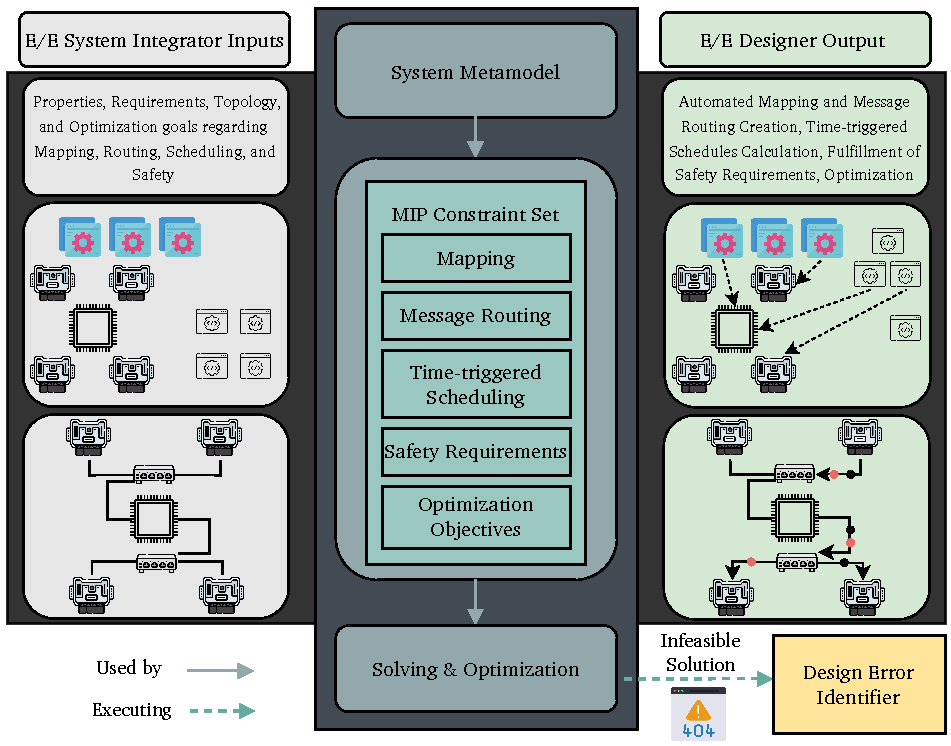
\includegraphics[width=1\textwidth]{figures/MainApproach.pdf}%{figures/approach_over1.pdf}%
    	%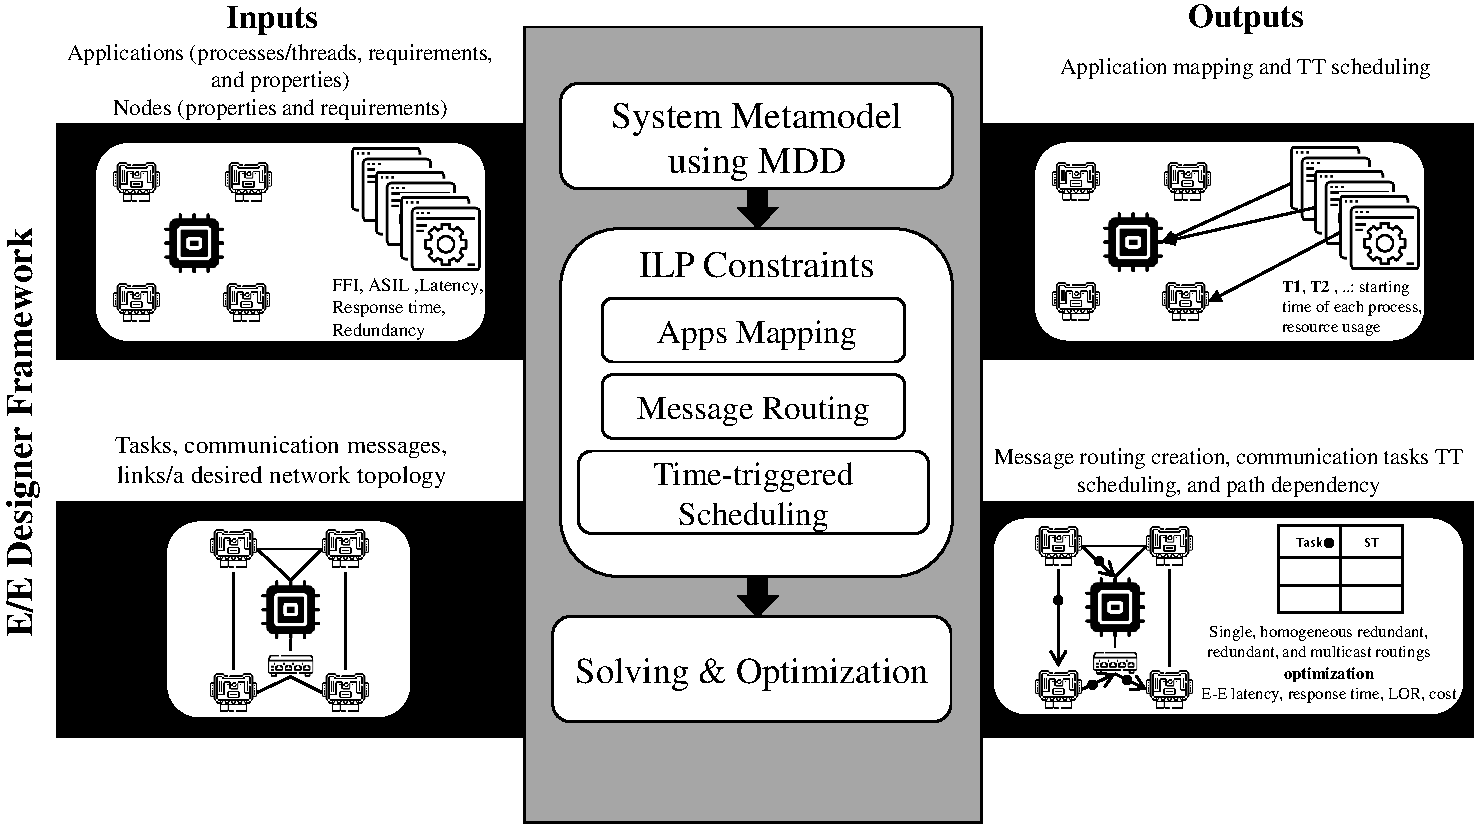
\includegraphics[width=8in]{approachnew.pdf}
    	\caption{The architecture of the proposed model-based framework. The left and right columns, representing E/E System Integrator Inputs and the E/E Designer Output, respectively, constitute the frontend. The middle box denotes the backend of the tool. In the framework's frontend, an E/E architecture is modeled by an E/E system architect. This modeling includes defining requirements, properties, and addressing various problems. The modeled E/E architecture is transformed into MIP formulations using the MDD approach. These formulations are then solved and optimized in the tool's backend. Finally, the optimal solution is visualized in the frontend of the framework.}
    	\label{fig041}
    \end{figure}
    %\vspace{-15pt}
    
    %Finally, after the solving step, the E/E Designer framework provides automated mapping or resource allocation (e.g., the automatic assignment of various application threads to different cores of a multi-core HPCU) and message routing creation (i.e., finding a correct path from the sender of a communication message to its receiver) for a modeled E/E architecture or network topology that satisfies the prespecified requirements as outputs. Additionally, the E/E Designer also computes time-triggered schedules for assigned running application threads on, e.g., a HPCU with multi-core architecture as well as communication tasks routing over car's network links. The created solution, as the tool's output, meets all requirements selected by the E/E system modeler and also it is optimized based on the chosen optimization goals.
    
    Finally, after the solving step, the E/E Designer framework provides automated mapping or resource allocation (e.g., automatically assigning various application threads to different cores of a multi-core HPCU) and creates message routes (i.e., finding the correct path from the sender of a communication message to its receiver) for a modeled E/E architecture or network topology that satisfies the predetermined requirements. Furthermore, the E/E Designer computes time-triggered schedules for the assigned running application threads, for example, on a multi-core HPCU, and manages communication task routing over the car's network links. The resulting solution, as the tool's output, fulfills all requirements selected by the E/E system modeler and is optimized based on the chosen optimization goals.
    

    %Furthermore, in case of having a feasible solution, a design error identifier approach (the yellow box in figure~\ref{fig041}) is executed to find the most related constraints which make the source of conflicts. This approach considerably facilitate the process of finding the violated constraints which is really elaborate and time-consuming with a large number of conditions.
    %Moreover, in the case of having a feasible solution, a design error identifier approach (the yellow box in Figure~\ref{fig041}) is executed to find the most related constraints that cause the source of conflicts. This approach considerably facilitates the process of finding the violated constraints, which is really elaborate and time-consuming with a large number of conditions. This refers to the second research question defined in the Chapter~\ref{intro}.
    
    Moreover, in the event of a feasible solution, an error identification approach (depicted by the yellow box in Figure~\ref{fig041}) is invoked to locate the constraints most likely responsible for conflicts. This approach significantly assists the task of identifying violated constraints, which can be an intricate and time-intensive process, especially when dealing with a substantial number of conditions. This pertains to the second research question outlined in Chapter~\ref{intro}.

   
	\subsection{Model-Driven Development}
	%Using MDD, software developers can build elaborate applications in a visualized manner because it utilizes pre-construct application components and graphical models. Automation of the challenging programming tasks  is defined as the main goal of MDD.	Furthermore, particularly when developing several applications, it speeds up the redeployment, rebuilds, and tests procedures compared with traditional approach~\cite{atkinson2003model}. There are various types of MDD tools for creating models for software design purposes using unified modeling language (UML).
	Model-driven development (MDD) is a software development methodology that has gained popularity in recent years due to its ability to increase development efficiency and reduce errors. MDD is based on the idea that software development can be greatly improved through the use of visual models and pre-constructed application components. This approach allows developers to focus on the high-level design of an application rather than the low-level details of programming. MDD provides a structured and standardized approach to software development, which makes it easier for developers to create complex applications quickly and accurately. Instead of writing code from scratch, developers use graphical models to describe the behavior and structure of the application. These models can then be automatically transformed into executable code using specialized tools~\cite{selic2003pragmatics, hailpern2006model}.
	
	Advantages of model-based development include:
    \begin{itemize}
        \item Increased efficiency: By using models to represent the system, developers can analyze and design the system more quickly and accurately than if they had to do so manually. This can lead to shorter development cycles and faster time to market.
        \item Improved quality: Models can help developers identify and fix problems early in the development process, reducing the risk of defects in the final product.
        \item Enhanced communication: Models can be used to communicate complex ideas and designs to stakeholders, making it easier for everyone involved in the development process to understand the system.
        \item Reusability: Models can be reused and repurposed for different projects, which can save time and effort in the development process.
    \end{itemize}
	With MDD, software developers can create sophisticated applications through the use of pre-constructed application components and graphical models. MDD's primary objective is to automate challenging programming tasks. In addition, this method can speed up the redeployment, rebuild, and testing procedures, especially when developing multiple applications, compared to the traditional approach~\cite{atkinson2003model}. 
    %Considering all above advantages regarding the MDD; therefore, this approach is utilized for the introduced framework by developing a system metamodel to build the basis for the graphical modeler. 
    Considering all the aforementioned advantages of MDD, this approach has been employed in the presented framework by developing a system metamodel to serve as the foundation for the graphical modeler.
    There are various types of MDD tools available for creating models for software design purposes. In this work, an open-source graphic modeling tool that employs unified modeling language (UML)~\cite{medvidovic2002modeling} from \textit{Eclipse Foundation} was utilized~\cite{9565115,askaripoor2023designer, eclipse}. 
    
    %Using a similar approach, the authors of~\cite{b13} present a model-based framework to facilitate schedule synthesis in TSN. 

	%Various types of MDD tools are available for creating models for software design purposes, using the Unified Modeling Language (UML)~\cite{9565115}.
	

	
    %One of the primary benefits of MDD is that it enables developers to rapidly create and modify software applications. Because the models are visual and abstract, developers can quickly prototype different ideas and experiment with different design choices. This allows for a more iterative and collaborative approach to software development, which can result in better quality software products that meet the needs of stakeholders. Moreover, MDD promotes code reuse, as pre-constructed application components can be easily incorporated into new projects. This not only speeds up the development process but also reduces the likelihood of errors and inconsistencies across different software projects~\cite{de2013software}.
	
	
%-------------------------------------------addition description. Must be checked-------------------------------------------------------	
	
	%Model-based development is a software development approach that relies on the use of models to represent and design software systems. It involves creating abstract representations of the system being developed, which can be used to analyze, design, and validate the system before it is implemented in code.Advantages of model-based development include:Increased efficiency: By using models to represent the system, developers can analyze and design the system more quickly and accurately than if they had to do so manually. This can lead to shorter development cycles and faster time to market.Improved quality: Models can help developers identify and fix problems early in the development process, reducing the risk of defects in the final product.Enhanced communication: Models can be used to communicate complex ideas and designs to stakeholders, making it easier for everyone involved in the development process to understand the system.Reusability: Models can be reused and repurposed for different projects, which can save time and effort in the development process.
    
    %Some potential disadvantages of model-based development include:Initial overhead: Creating and maintaining models can be time-consuming, which can add additional overhead to the development process.Complexity: Model-based development can be complex, especially for larger or more complex systems. This can make it difficult for some developers to understand and work with the models.Limited flexibility: The use of models can also limit flexibility in the development process, as changes to the model may require significant effort to implement.Dependence on tools: Model-based development often relies on specialized tools and software to create and work with the models, which can be an additional cost and may require training and resources to use effectively.

    %\subsection{Model-Driven Development}

    %There are various types of MDD tools for creating models for software design purposes. In this work, an open-source graphic modeling tool using Unified Modeling Language (UML) from \textit{Eclipse Foundation}  was utilized. Using a similar approach, the authors of~\cite{b13} present a model-based framework to facilitate schedule synthesis in TSN. The framework automates the creation and solving of scheduling constraints for the safety-critical network traffic.
    %%----------------------------------------------------another explanation--------------------------------------------------------
 
    
    %Overall, model-based development provides a structured and organized approach to software development, which can help to reduce the risk of errors and improve the quality of the final product.

%E/E Designer are automated mapping of HW/SW components, calculation of time-triggered schedules for mapped processes/threads, automatic message routing generation comprising single, redundant, homogeneous redundant, and multi-cast routes, time-triggered computation for communication tasks,and path and message dependency for each communication message chain. In addition, various optimization goals, including end-to-end latency, response time, resource usage, link occupation rate (LOR), cost, and multi-objective optimizationare integrated into the set of constraints. To solve and optimize the ILP constraints in the E/E Designer system model, aGurobi optimization solver is utilized [19]. After the solvingstep, a solution regarding all the defined constraints as theoutput of E/E Designer is created and visualized by the frontend.

 

    \subsection{Object-oriented Metamodel}\label{metamodel}
    %A metamodel is a model that defines the structure, elements, and relationships of other models.An object-oriented metamodel is a fundamental concept that defines how UML itself is structured and represented. It essentially provides a set of rules and constructs for defining UML elements and their relationships.   This typically involves representing and defining modeling elements and relationships using object-oriented concepts such as classes, objects, attributes, methods, and inheritance. This metamodel provides a structured way to define and organize the elements and semantics of a modeling language, making it easier to create, understand, and manipulate models in a consistent and modular manner~\cite{hailpern2006model, medvidovic2002modeling, 9565115}. 
    
    A metamodel is a model that defines the structure, elements, and relationships of other models.
    An object-oriented metamodel is a fundamental concept that defines how UML itself is structured and represented. It essentially provides a set of rules and constructs for defining UML elements and their relationships. This typically involves representing and defining modeling elements and relationships using object-oriented concepts such as classes, objects, attributes, methods, and inheritance. Such a metamodel provides a structured approach to define and organize the elements and semantics of a modeling language, simplifying the process of creating, comprehending, and manipulating models in a consistent and modular manner~\cite{hailpern2006model, medvidovic2002modeling, 9565115}.
    
    
    
    %A metamodel is developed for the proposed tool, as shown in figure~\ref{fig042}, to build the basis for the graphical modeler. 
    %It consistsof a network view which contains all graphical network components. A network node is either aswitch or an end-station. Nodes consist of at least one Ethernet port. Switches and end-stationsare connected through ports. A link connects two nodes and has exactly one source and onetarget port. 	

      	



    A metamodel is developed for the proposed tool, as depicted in Figure~\ref{fig:metamodel}, building the foundation for the graphical modeler.
    The developed metamodel, which employs UML to describe another model as an instance, comprises 39 elements. This metamodel includes 33 classes, with 14 of them serving as the primary classes within the system model. These 14 key elements encompass Node, Application, Link, Data, Data\_in, Data\_out, Process, Task, Mapping, ECU, Processor, Core, Hypervisor, and Settings.
    Furthermore, the metamodel encompasses various attribute types, including ASIL level, memory, optimization goal, link, and node types. It also includes a data type used by the system model's elements for the Gurobi solver, which serves as a MIP solving engine~\cite{gurobi}.
    In the following paragraph, the relationships between primary classes, as illustrated in Figure~\ref{fig:metamodel}, are explained    
    
    %Node class includes several attributes and types. Node's types comprise ECU, HPCU, gateway, and network switch. Each Node can include \textit{one-to-many} links, \textit{zero-to-many} applications as the sender and the receiver, and \textit{zero-to-many} mappings. Mapping refers to the mapping action or resource allocation.
    
    According to Figure~\ref{fig:metamodel}, the Node class encompasses several attributes and types. Node types include ECU, HPCU, gateway, and network switch. Each Node can have \textit{one-to-many} links, \textit{zero-to-many} applications as both senders and receivers, and \textit{zero-to-many} mapping elements. Mapping class refers to the action of mapping or resource allocation.
    %Application class can have \textit{zero-to-many} processes, and it has a \textit{one-to-one} relation with the Mapping class meaning that each application owns an unique mapping attribute. Each process is related to only one application and each application process can only send/receive one communication message or Data according to the figure~\ref{fig042}. 
    The Application class can have \textit{zero-to-many} processes and maintains a \textit{one-to-one} relationship with the Mapping class, signifying that each application has a unique mapping attribute. Each process is associated with only one application, and each application process can send/receive only one communication message indicated as Data class in Figure~\ref{fig:metamodel}.
    %Each communication message (in figure~\ref{fig042} Data) includes \textit{one-to-many} communication tasks and can be received by one or multiple application processes while it can be sent only by one process. 
    Each communication message consists of a \textit{one-to-many} relationship with communication tasks (depicted in Figure~\ref{fig:metamodel} under as Task), meaning it can be received by one or multiple application processes but can only be sent by one process.
    %Moreover, each communication message has \textit{one-to-many} relation with outgoing and incoming messages which are named Data\_Out and Data\_In, respectively, according to the metamodel shown in figure~\ref{fig042}~\cite{9565115}. 
    Furthermore, each communication message exhibits a \textit{one-to-many} relationship with outgoing and incoming messages, denoted as Data\_Out and Data\_In, respectively, in accordance with the metamodel presented in Figure~\ref{fig:metamodel}. Furthermore, there exists a bidirectional reference between each Data\_In and Data\_Out~\cite{9565115}.
    %Also, each Data\_In is referenced to each Data-out and conversely. 
    %A communication link has two \textit{one-to-one} relations with the Node as starting and finishing points of each link. Besides, each Link can have \textit{one-to-many} communication tasks, and outgoing and incoming messages. Note that each communication task is only related to one link.
    A communication link has two \textit{one-to-one} relations with the Node, serving as the starting and finishing points of each link. Additionally, each Link can have \textit{one-to-many} communication tasks and outgoing and incoming messages. It is important to note that each communication task is associated with only one link.
    %Settings class includes several attributes regarding different requirements such as reliability and message routing, boundary goals, optimization objectives, and visualization-related options, i.e., showing desired mapping solutions for applications and paths for communication messages. 
    The Settings class includes several attributes related to different requirements, such as reliability, message routing, boundary goals, optimization objectives, and visualization-related options. This incorporates the display of desired mapping solutions for applications and paths for communication messages.
    Each ECU, as a type of node, can own \textit{zero-to-many} processors (where each processor can have \textit{zero-to-many} cores) and memories. In the case of an HPCU, the same relationships apply. Moreover, an HPCU can own \textit{zero-to-many} GPUs, hypervisors, and partitions~\cite{9565115,askaripoor2023designer}.
    
    %Each ECU, as a type of a node, can own \textit{zero-to-many} processors (each processor can have \textit{zero-to-many} cores) and memories. For an HPCU, the same relations is applied; in addition, it can own \textit{zero-to-many} GPUs, hypervisors, and partitions~\cite{9565115,askaripoor2023designer}. 
    
    
    
    %either as the sender or the receiver, can only be mapped on one Node; moreover, the Application can only send one Data based on \textit{one-to-one} reference relation with Data. Furthermore, each pair of applications are considered ($A_{sen}, A_{rec}$) as one application in our run-time evaluation. In our designed metamodell (figure \ref{fig1}), a Link (with the same role as explained in $G_{Arch}$) can be referenced to a Node as its starting point and its finishing point. In addition, \textit{one-to-many} Data-{In} and Data-{Out} can be routed over a Link. In this class diagram, Data, which is described in $G_{App}$ as our system model, references to \textit{one-to- many} Data-In and Data-Out while it can be either sent or received by only one Application. Eventually, according to figure \ref{fig1}, Data-In or Data-Out (described in $G_{App}$ as well as \ref{B}) can be routed over only one Link; moreover, each Data-In or Data-Out belongs to a Data. Also, each Data-In is referenced to each Data-out and conversely.
    
    
    %According to figure \ref{fig042}, the developed metamodel (i.e., using a model to describe another model as an instance) of our framework is visualized. This metamodell consists of eight elements. The Topology element plays a role as the main class of the metalmodell where all other classes are subordinate to it. 
    
   
    
    
    %We develop a network metamodel to build the basis for the graphical modeler [133]. It consistsof a network view which contains all graphical network components. A network node is either aswitch or an end-station. Nodes consist of at least one Ethernet port. Switches and end-stationsare connected through ports. A link connects two nodes and has exactly one source and onetarget port.A real-time application is presented as a domain in the metamodel. Each domain containsone or more data topics which are published and consumed through ports within a domain.

	
	
     %MDD enables developers to create high-quality software in less time and with fewer errors. It allows for the rapid production of code, which can then be tested and refined, resulting in a more efficient software development process. Moreover, MDD enables software developers to create complex applications with ease, as it provides a structured and standardized approach to software design.
    
    %Another advantage of MDD is that it promotes collaboration between developers and stakeholders. Through the use of visual models, MDD allows for easier communication of software requirements and specifications. This helps to ensure that everyone involved in the software development process has a clear understanding of the project's goals and objectives, which can lead to a more successful outcome.
    
    %In conclusion, MDD is a powerful software development methodology that can help developers create complex applications with ease, while promoting collaboration and reducing the likelihood of errors. By using MDD, developers can streamline their development processes, increase their efficiency, and deliver high-quality software products to their clients.
	
	
	
	%(e.g., preparing support for system distribution, interoperability, and persistence)
	
	%Automation and abstraction build the core concepts of this approach so that the abstraction level specifies the software application model and afterward by utilizing automated interpretations, the application model is transformed into a functioning application. The model execution is handled during the execution time once using MDD in such a way that it is converted into an operating application automatically through model explanation and execution; to be more clear, there is no need to write or generate any codes. MDD operates more in-depth which is interpreted as the difference between MDD and model-based development. %\cite{b9}. The engineering procedure is made easier by the MDD approach, and it is also the reason for precedence in productivity over other development methods. The behaviours of the software product are demonstrated prior to coding.
 
	%There are various types of MDD tools for creating models for software design purposes. In this work, an open-source graphic modeling tool using Unified Modeling Language (UML) from \textit{Eclipse Foundation}  was utilized. Using a similar approach, the authors of~\cite{b13} present a model-based framework to facilitate schedule synthesis in TSN. The framework automates the creation and solving of scheduling constraints for the safety-critical network traffic.
	
	%According to figure \ref{fig1}, the designed metamodell ( i.e., using a model to describe another model as an instance) of our framework is visualized. This metamodell consists of eight elements. The Topology element plays a role as the main class of the metalmodell where all other classes are subordinate to it. Here we have five classes as the main elements in our system model including Node, Application, Link, Data, Data-in, and Data-out; in addition, there is a data type (i.e., GRBTopology) used by the elements of the system model. To explain the relation of each element to the system model mentioned in \ref{sys}, Node class plays the same role as the node in the $G_{Arch}$ and includes several attributes. Here, each Node can include \textit{one-to-many} links and \textit{zero-to-many} applications as the sender and the receiver. While Application, similarly presented in $G_{App}$, either as the sender or the receiver, can only be mapped on one Node; moreover, the Application can only send one Data based on \textit{one-to-one} reference relation with Data. Furthermore, each pair of applications are considered ($A_{sen}, A_{rec}$) as one application in our run-time evaluation. In our designed metamodell (figure \ref{fig1}), a Link (with the same role as explained in $G_{Arch}$) can be referenced to a Node as its starting point and its finishing point. In addition, \textit{one-to-many} Data-{In} and Data-{Out} can be routed over a Link. In this class diagram, Data, which is described in $G_{App}$ as our system model, references to \textit{one-to- many} Data-In and Data-Out while it can be either sent or received by only one Application. Eventually, according to figure \ref{fig1}, Data-In or Data-Out (described in $G_{App}$ as well as \ref{B}) can be routed over only one Link; moreover, each Data-In or Data-Out belongs to a Data. Also, each Data-In is referenced to each Data-out and conversely.

	
	%\subsubsection{Model-Driven Development}
	
	
	%(e.g., preparing support for system distribution, interoperability, and persistence)
	
	%Automation and abstraction build the core concepts of this approach so that the abstraction level specifies the software application model and afterward by utilizing automated interpretations, the application model is transformed into a functioning application. The model execution is handled during the execution time once using MDD in such a way that it is converted into an operating application automatically through model explanation and execution; to be more clear, there is no need to write or generate any codes. MDD operates more in-depth which is interpreted as the difference between MDD and model-based development. %\cite{b9}. The engineering procedure is made easier by the MDD approach, and it is also the reason for precedence in productivity over other development methods. The behaviours of the software product are demonstrated prior to coding.
 
	
	
	%According to figure \ref{fig1}, the designed metamodell ( i.e., using a model to describe another model as an instance) of our framework is visualized. This metamodell consists of eight elements. The Topology element plays a role as the main class of the metalmodell where all other classes are subordinate to it. Here we have five classes as the main elements in our system model including Node, Application, Link, Data, Data-in, and Data-out; in addition, there is a data type (i.e., GRBTopology) used by the elements of the system model. To explain the relation of each element to the system model mentioned in \ref{sys}, Node class plays the same role as the node in the $G_{Arch}$ and includes several attributes. Here, each Node can include \textit{one-to-many} links and \textit{zero-to-many} applications as the sender and the receiver. While Application, similarly presented in $G_{App}$, either as the sender or the receiver, can only be mapped on one Node; moreover, the Application can only send one Data based on \textit{one-to-one} reference relation with Data. Furthermore, each pair of applications are considered ($A_{sen}, A_{rec}$) as one application in our run-time evaluation. In our designed metamodell (figure \ref{fig1}), a Link (with the same role as explained in $G_{Arch}$) can be referenced to a Node as its starting point and its finishing point. In addition, \textit{one-to-many} Data-{In} and Data-{Out} can be routed over a Link. In this class diagram, Data, which is described in $G_{App}$ as our system model, references to \textit{one-to- many} Data-In and Data-Out while it can be either sent or received by only one Application. Eventually, according to figure \ref{fig1}, Data-In or Data-Out (described in $G_{App}$ as well as \ref{B}) can be routed over only one Link; moreover, each Data-In or Data-Out belongs to a Data. Also, each Data-In is referenced to each Data-out and conversely. 


    \subsection{Constraint Set}
    
    \subsubsection{Constraint Satisfaction Problem}
    Constraint satisfaction problem or CSP is a type of problem in computer science, artificial intelligence, and mathematics that involves finding a solution to a set of constraints or conditions. In a CSP, the problem is typically defined by a set of variables, each with a corresponding set of possible values or domains and a set of constraints that must be satisfied by the variables' values. The goal of the problem is to discover a consistent assignment of values to the variables that fulfills all the constraints.
    %CSPs have many applications, including in scheduling, resource allocation, planning, and design. They are used in a variety of fields, including computer science, operations research, artificial intelligence, and engineering. Solving a CSP can be a complex process, as the number of possible solutions can be very large, and finding a solution that satisfies all the constraints can be difficult. There are many algorithms and techniques that have been developed to solve CSPs efficiently, including backtracking, forward checking, and constraint propagation~\cite{poole2010artificial, russell2010artificial}.
    CSPs have numerous applications, including scheduling, resource allocation, planning, and design. They find use in various fields, such as computer science, operations research, artificial intelligence, and engineering. Solving a CSP can be complex due to the potentially vast number of solutions and the challenge of satisfying all constraints. Many algorithms and techniques have been developed to efficiently solve CSPs, including backtracking, forward checking, and constraint propagation~\cite{poole2010artificial, russell2010artificial}.
    
    A constraint satisfaction problem includes three components, $X$, $D$, and $C$ where 
    $X$ is a set of variables, $\{X_1,...,X_n\}$,
    $D$ is a set of domains, $\{D_1,...,D_n\}$, one for each variable, and 
    $C$ is a set of constraints that specify allowable combinations of values~\cite{russell2010artificial}.
    
    
    \subsubsection{ILP and LP}
    In integer linear programming (ILP) or integer programming (IP), all the decision variables are required to be integers, whereas in linear programming (LP), all the decision variables are continuous. ILP is a type of optimization problem where the objective function and constraints are linear, but some or all of the decision variables are restricted to be integers~\cite{vanderbei2020linear}. %In contrast to linear programming, which can be solved efficiently in the worst case, integer programming problems are in many practical situations (those with bounded variables) NP-hard. 0–1 integer programming or binary integer programming (BIP) is the special case of integer programming where variables are required to be 0 or 1 (rather than arbitrary integers). This problem is also classified as NP-hard, and in fact the decision version was one of Karp's 21 NP-complete problems.
    While LP can be efficiently solved in the worst case, IP problems can pose significant challenges in many practical situations. This is particularly true for problems with bounded variables, where the number of possible solutions is limited. As a result, integer programming problems are often classified as NP-hard. NP-hard problems are a class of computational problems that are at least as hard as the hardest problems in the complexity class NP. The abbreviation NP stands for nondeterministic polynomial time, which refers to the set of decision problems that can be solved by a nondeterministic Turing machine in polynomial time.
    An NP-hard problem is a problem that is at least as difficult as any problem in NP. In other words, if an NP-hard problem can be solved in polynomial time, then every problem in NP can also be solved in polynomial time. This is because an NP-hard problem can be reduced to any problem in NP in polynomial time.
    There are many important computational problems that are known to be NP-hard, including the traveling salesman problem, the knapsack problem, and the Boolean satisfiability problem. These problems have important applications in fields such as operations research, computer science, and artificial intelligence~\cite{fortnow2009status}.

    One special case of integer programming is 0-1 integer programming, also known as binary integer programming (BIP). In this type of problem, variables are restricted to take on values of either 0 or 1 rather than arbitrary integers. Despite this restriction, 0-1 integer programming is still classified as NP-hard and is known to be one of Karp's 21 NP-complete problems. The decision version of 0-1 integer programming involves determining whether there exists a feasible solution that satisfies a given set of constraints. This decision problem is known to be NP-complete, meaning that it is at least as hard as any other NP problem and cannot be solved in polynomial time. However, despite the theoretical difficulty of solving 0-1 integer programming problems, there exist powerful algorithms and techniques that can be used to find good approximate solutions in practice~\cite{vanderbei2020linear, garey1974some}.

    \subsubsection{MIP and MILP}
    %\footnote{Mentioning Difference between MIP and MILP}
    MIP is a more general type of optimization problem, where some of the decision variables can be continuous, and others can be restricted to be integers. It can contain both integer and continuous variables. MIP is also able to include quadratic constraints; in other words, it combines the features of both LP and ILP.  
    MIP problems can be more challenging to solve than LP or ILP problems, as including integer and continuous variables can make the problem non-convex and non-linear, leading to a more complex solution process. 
    
    Mixed-integer linear programming (MILP) is a subset of MIP where all variables, whether continuous or integer, have linear relationships in both the objective function and constraints.
    In MILP, the objective function and constraints are linear, but some or all of the decision variables can be integers, binary (0 or 1), or a combination of both.
    MIP and MILP are widely used in various fields, including operations research, engineering, finance, and economics. They are a powerful tool for solving many real-world optimization problems, such as production planning, scheduling, resource allocation, transportation planning, and portfolio optimization. MIP and MILP can help decision-makers to make better decisions by optimizing a wide range of objective functions, such as minimizing cost, maximizing profit, or maximizing efficiency~\cite{junger200950,vanderbei2020linear}. These problems are generally also NP-hard because they are even more general than ILP programs.
    Mixed-integer linear programs are problems that can be expressed in canonical form as follows:
    %\vspace{5mm}
    \begin{equation*}
        min_{x, y}\;\;\;\;  c^{T} x + h^{T} y
    \end{equation*}
    
    subject to:
    \begin{equation*}
        A x + G y \geq b
    \end{equation*}
    \begin{equation*}
        (x, y) \in \mathbb{R}^{n}_{+} \times \mathbb{Z}^{p}_{+}
    \end{equation*}
    where $A$ and $G$ are $m \times n$ and  $m \times p$ matrices, respectively. Moreover, $b$, $c$, and $h$ represent $m$-, $n$-, and $p$-dimensional vectors, respectively. In the last constraint, $\mathbb{R}^{n}_{+}$ is the $n$-dimensional space of all non-negative real numbers ($\mathbb{R}^{n}_{+} = \{ x \in \mathbb{R}^{n} : x\geq 0 \}$) and $ \mathbb{Z}^{p}_{+}$ is the $p$-dimensional space of all non-negative integer numbers ($\mathbb{Z}^{n}_{+} = \{ y \in \mathbb{Z}^{n} : y\geq 0 \}$). Accordingly, a set of feasible solutions can be defined below as $X$:
    \begin{equation*}
        X = \{ (x, y) \in \mathbb{R}^{n}_{+} \times \mathbb{Z}^{p}_{+} :  A x + G y \geq b\}
    \end{equation*}
    In the following, a simple mathematical example of MILP is presented :
    
    \begin{equation*}
        max:\;\;\;  x + y
    \end{equation*}
    subject to:
    \begin{equation*}
           C_1 : -2x + 2y \geq 1
    \end{equation*}
    \begin{equation*}
        C_2 :  8x - 10y \leq 13
    \end{equation*}
    \begin{equation*}
         C_3 : x, y \geq 0 
    \end{equation*}
    \begin{equation*}
         C_4 : x, y \in \mathbb{R}  
    \end{equation*}
      
    
    %In this example, $x$ and $y$ are decision variables that the optimal values are intended to be found for. The objective function wants to be maximized is $x + y$. The first two constraints ($C_1$ and $C_2$) are linear inequalities that restrict the possible values of $x$ and $y$. The third and forth constraints ($C_3$ and $C_4$) specify that $x$ and $y$ must be greater than zero and they belong to real numbers, respectively.
    In this example, $x$ and $y$ are decision variables for which the optimal values are sought. The objective function to be maximized is $x + y$. The first two constraints ($C_1$ and $C_2$) are linear inequalities that restrict the possible values of $x$ and $y$. The third and fourth constraints ($C_3$ and $C_4$) specify that $x$ and $y$ must be greater than zero, and they belong to the set of real numbers, respectively.
    %One approach to solving this MILP problem is to use a branch and bound algorithm. This algorithm works by branching on the integer variables, creating subproblems that are each a smaller version of the original problem. The algorithm solves each subproblem by applying linear programming techniques, and then determines whether the solution is integer feasible. If the solution is not integer feasible, the algorithm branches further and repeats the process until an integer feasible solution is found~\cite{lawler1966branch}. Therefore, the optimal solution of its LP relaxation is $(x, y) = (4 , 4.5)$ with objective $ 8.5$ using branch and bound algorithm.
    One approach to solving this MILP problem is to use a branch and bound algorithm. This algorithm works by branching on the integer variables, creating subproblems, each of which is a smaller version of the original problem. The algorithm solves each subproblem by applying linear programming techniques and then determines whether the solution is integer-feasible. If the solution is not integer-feasible, the algorithm branches further and repeats the process until an integer-feasible solution is found~\cite{lawler1966branch}. Therefore, the optimal solution of its LP relaxation is $(x, y) = (4, 4.5)$ with an objective value of $8.5$ using the branch and bound algorithm.
    
    
    
    
    
    
    %For example, suppose we start by solving the linear programming relaxation of the problem, where we ignore the integer constraints on $x$, $y$, and $z$. The linear programming relaxation is:
    
    %One of the key challenges of MIP and MILP is finding an optimal solution in a reasonable amount of time. These problems are generally more complex and computationally intensive than LP or IP problems due to the inclusion of integer variables. Solving an MIP problem involves exploring a large solution space and requires a combination of mathematical algorithms and computational methods. To solve MIP problems, various software packages are available, such as Gurobi, CPLEX, and GLPK~\cite{gurobi,cplex2009v12,AMakhorin}. These software packages use advanced algorithms and optimization techniques, such as branch-and-bound, cutting planes, and heuristics, to find an optimal solution or a near-optimal solution within a reasonable amount of time.
    One of the key challenges of MIP and MILP is to find an optimal solution within a reasonable time frame. These problems are generally more complex and computationally intensive than LP or IP problems due to the inclusion of integer variables. Solving a MIP problem involves exploring a large solution space and requires a combination of mathematical algorithms and computational methods.
    To solve MIP problems, various software packages are available, such as Gurobi, CPLEX, and GLPK~\cite{gurobi, cplex2009v12, gnu}. These software packages employ advanced algorithms and optimization techniques, including branch-and-bound, cutting planes, and heuristics, to discover an optimal solution or a near-optimal solution within a reasonable amount of time.
    
    
    
    
    %Based on the above explanation, we use MIP programming to formulate our problems and requirements, including mapping, message routing, time-triggered scheduling, message and path dependencies, and safety-related conditions and transform them into constraints. Furthermore, the Gurobi MILP solver~\cite{gurobi} is utilized to solve these constraints~\cite{9565115, askaripoor2023designer}. The formulation of these constraints and their details will be explained in the following sections.
    Based on the explanation provided above, MIP is employed to formulate the problems and requirements presented in this thesis. These encompass tasks such as mapping or resource allocation, message routing, time-triggered scheduling, addressing message and path dependencies, and ensuring safety-related conditions. These requirements are then transformed into a set of constraints. To solve these constraints, the Gurobi MILP solver~\cite{gurobi} is utilized as referenced in~\cite{9565115, askaripoor2023designer}. The forthcoming sections will detail the formulation of these constraints and provide additional insights into their specifics.

    \subsection{Optimization}
    To apply MIP to the synthesis of E/E architecture, the problem must first be formulated as a mathematical model, as mentioned before. This involves identifying the variables, constraints, and optimization goals of the problem.
    Once the model is formulated, the optimization goals can be specified~\cite{9565115,9613692}.
    In the automotive domain, a system model can be used to optimize the performance of various components and systems in a vehicle. A system model is a representation of a complex system that can be used to simulate and analyze its behavior under different conditions. Optimization involves finding the best possible set of inputs or parameters to achieve a specific goal or objective.
    These goals may include minimizing the cost of the architecture, maximizing its reliability, or optimizing its performance. Different optimization goals will result in different optimal solutions, so it is essential to choose the goals carefully based on the specific requirements of the E/E architecture. For instance, cost optimization can be used to reduce the cost of production and operation of a vehicle by optimizing the design of the components and systems to reduce material and labor costs, and improve efficiency.
    
    Once the optimization goals are specified, the MIP solver can be used to solve the optimization problem and generate an optimal solution. The solver searches for the values of the variables that minimize or maximize the optimization goals while satisfying the constraints of the model. In the introduced framework, several optimization objectives are integrated, including cost reduction (CR), end-to-end latency, response time, resource utilization (RU), load balancing in-vehicle communication network, and reliability. In addition, the introduced tool supports multi-objective optimization as well. The details of all these objectives will be described in Section~\ref{opt_goals}.


    \subsection{Design Error Identifier}
    
    As depicted earlier, based on the yellow box in Figure~\ref{fig041}, it is common to encounter infeasible solutions while solving a constraint system. Tackling this problem can be difficult and time-consuming, particularly with many constraints or conditions involved. To overcome this challenge, an approach to identify violated constraints can help E/E system architects identify conflicts' sources early in the design process, allowing them to navigate towards a feasible solution more efficiently. Therefore, an approach is introduced called the design error approach, which uses infeasible inconsistent subsystem (IIS) and minimal unsatisfiable cores (MUC). A MUC is a subset of the negation of the constraint that is itself unsatisfiable, i.e., no assignment of variables can make all of the clauses in the MUC true. The MUC gives information about which parts of the negation of the constraint are causing the violation. IIS is also similar to MUC. This information can pinpoint the violated part of the original constraint used in the approach. Specifically, the negation of the MUC can be taken and intersected with the original constraint to obtain a minimal set of clauses responsible for the violation~\cite{lynce2004computing, dershowitz2006scalable}. In Chapter~\ref{designerror}, this approach will be discussed in detail.
%\clearpage
    \begin{figure}[t]
    	\centering
    	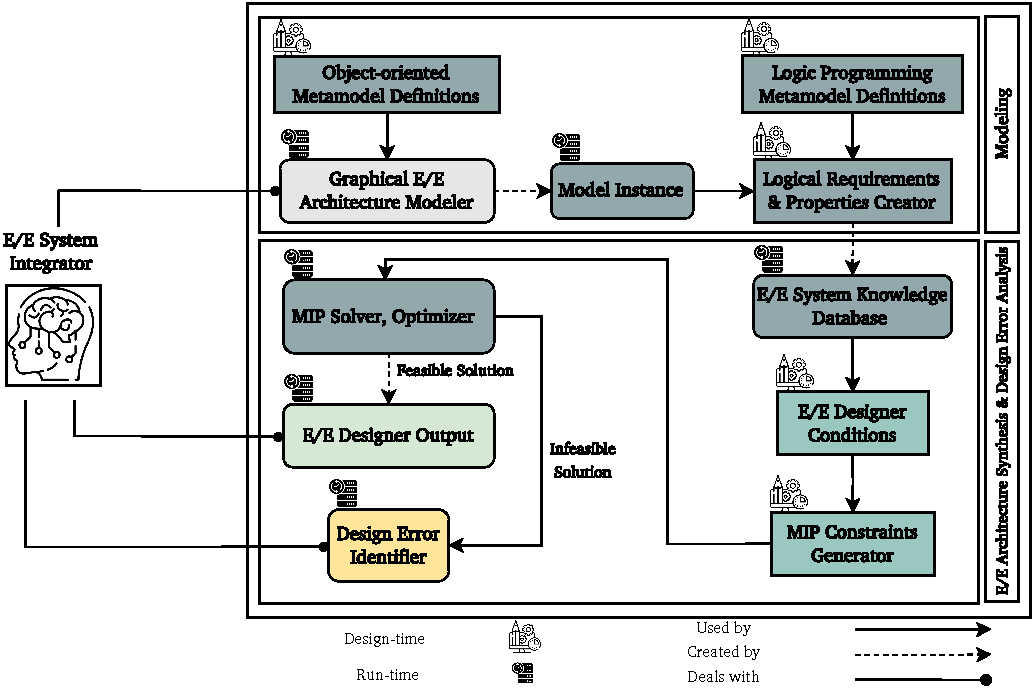
\includegraphics[width=1\textwidth]{figures/overview_tool.pdf}%
    	%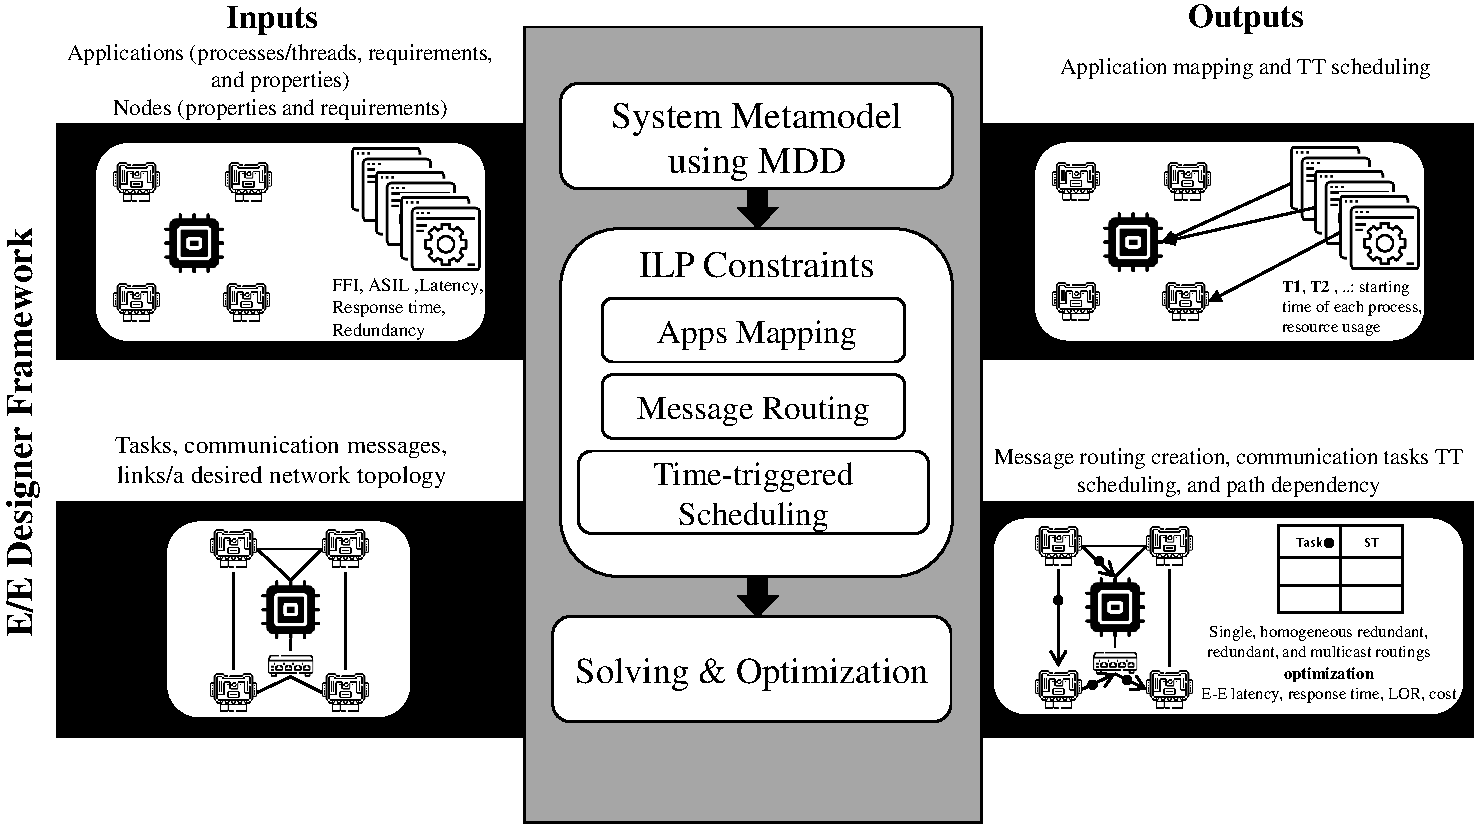
\includegraphics[width=8in]{approachnew.pdf}
    	\caption{The overview of the framework, including modeling, synthesis, and design error analysis parts.}
    	\label{fig043}
    \end{figure}
    \subsection{An Overview of Framework Architecture}
    In Figure~\ref{fig043}, the modeling approach involves an object-oriented metamodel, which serves as the foundation for a graphical E/E architecture modeler. This modeler enables the creation of visual representations of the model instances. E/E system integrators utilize the graphical modeler, which offers drag-and-drop functionality, to design car E/E systems. These systems consist of both hardware and software components, along with their corresponding physical properties.
    The user can specify timing requirements and choose from a range of safety conditions, boundary goals, and optimization objectives. For instance, it is possible to define an application that includes a thread with a specific period and execution time, designating it as a safety-critical application. This designation implies that redundancy requirements must be met during mapping and routing for this particular application.

%As depicted in figure~\ref{fig043}, the modeling approach consists of an object-oriented metamodel which builds the basis of a graphical E/E architecture modeler to create graphicalmodel instances. E/E system integrators use the graphical modeler (withdrag\&drop functionalities) to design car E/E systems comprising hardware and software components and their physical properties. The user can specify timing requirements and select various safety conditions as well as different boundary goals and optimization objectives. For example, it can be defined that an application contains a thread with a specific period and execution time and it is defined as a safety-critical application. Meaning that in case of mapping and routing for this application, redundancy requirement must be fulfilled.  

%periodic data transmission with tight timing constraints or it has reliability requirements and multiple disjoint paths (cf. IEEE 802.1CB) have to be provided. The modeling toolis also used to define the network topology and the physical properties of the components.

%Using a formal metamodel based on logic programming, the graphical model instances are transformed into a E/E system knowledge database. Considering the E/E system database, the conditions and requirements are extracted and transformed into MIP constraints which are mathematical formulations in the form of MIP. These constraints can include mapping problem, message routing, time-triggered scheduling, and various boundary and optimization objectives. Using a MIP solver and optimizer, the constraints are solved and it is decided whether there is a feasible solution for the designed model. If the solution become feasible, it is visualized for the E/E system integrator as \textit{E/E Designer} output. On the other hand, if the tool cannot solve the system model due to conflicts in the constraint set, the design error identifier approach is activated to find the most critical conditions which cause the source of violation. The output of this approach is also shown to the E/E system integrator.  

A formal metamodel based on logic programming is used to transform graphical model instances into a knowledge database for E/E systems. The E/E system database is analyzed to extract conditions and requirements, which are then converted into mathematical formulations called MIP constraints. These constraints cover mapping problems, message routing, time-triggered scheduling, boundary considerations, and optimization objectives. The constraints are solved using an MIP solver and optimizer to determine if a feasible solution exists for the designed model. If a feasible solution is found, it is presented as output for the E/E system integrator. However, if conflicts in the constraint set prevent the tool from solving the system model, the design error identifier approach is activated. This approach identifies the most critical conditions causing the violation and presents the findings to the E/E system integrator. In Figure~\ref{fig043}, run-time and design-time states for each step is visualized.

%.Therefore,.Moreover, inference rules (7)are developed to exploit the power of logical inference which are required to query and verify network properties such as path redundancy (9), andto transform the required information from the network model into time-triggered scheduleconstraints (8),(9).Using a Satisfiability Modulo Theories (SMT) solver, the constraints are solved and it will bedecided whether there is a feasible schedule for the model. The constraints can also be usedfor verification of manually created schedules. The solver checks the schedule and decides if allconstraints (real-time requirements) are fulfilled. These components are grouped and we call itTSN Declarative Network Management (DNM).


\section{Framework System Model}

%The \textit{E/E Designer} system model is a distributed system that consists of multiple nodes and links. We represent this system as a graph $G(N, L)$, with vertices $N$ representing vehicle nodes (such as HPCUs, ECUs, gateways, and network switches) and edges $L$ representing full-duplex links (such as Ethernet, FlexRay, and time-triggered CAN bus). Gateways and switches only act as networking or intermediate nodes to transfer data from one point to another. While HPCUs and ECUs can function as control nodes, where applications can be assigned and they can also send/receive data. Besides, the control nodes can also function as intermediate nodes.


The system model of the E/E Designer framework is a distributed system comprising multiple nodes and links. It can be depicted as a graph denoted as $G(N, L)$, where the vertices $N$ represent vehicle nodes (such as HPCUs, ECUs, gateways, and network switches), and the edges $L$ represent full-duplex links (like Ethernet, FlexRay, and time-triggered CAN bus). Gateways and switches function as intermediate or networking nodes, facilitating data transfer between different points. On the other hand, HPCUs and ECUs can function as control nodes, responsible for executing applications and sending or receiving data. Control nodes can also act as intermediate nodes~\cite{askaripoor2023designer}.


%Additionally, each HPCU may have sub-components, such as processors, cores, graphics processing units (GPUs), and memory. To distinguish between different types of nodes, we use the notation $n^{cz}$ to symbolize a control node and $n^{nz}$ to represent a networking node. A single core that belongs to a control node, such as an HPCU core, is denoted as $n^{cz_c}$.A full-duplex link between two nodes $n_a$ and $n_b$ is represented by $l_{a,b} \in L$ and $l_{b, a} \in L$, indicating directed links from $n_a$ to $n_b$ and from $n_b$ to $n_a$, respectively. The \textit{E/E Designer} system model includes several components, explained as follows.

Furthermore, each HPCU may consist of sub-components like processors, cores, GPUs, and memory. We use the notation $n^{cz}$ to differentiate between node types to indicate a control node and $n^{nz}$ to represent a networking node. A single core belonging to a control node, such as an HPCU core, is denoted as $n^{cz_c}$.
A full-duplex link connecting two nodes $n_a$ and $n_b$ is represented by $l_{a, b} \in L$ and $l_{b, a} \in L$, signifying directed links from $n_a$ to $n_b$ and from $n_b$ to $n_a$, respectively. The E/E Designer tool's system model encompasses several components, which are explained as follows~\cite{askaripoor2023designer, 9565115}.



\subsection{Application Thread}
%In our system model, each application running on a control node can have multiple processes/threads. A thread running on a control node is defined as an application thread. We assume that threads are periodic, denoted as $t_i$, and specified by a tuple $t_i$ $=$ \{$t_i.p$, $t_i.st$, $t_i.e$\}. The description of each element is explained in Table~I. In the example shown in figure~\ref{mapping}, there are four applications, each including one thread, running on $n_{1}^{cz}$.

In the proposed framework's system model, there can be multiple processes/threads for each application that runs on a control node. An application thread refers to a thread running on a control node. An assumption is made that these threads are periodic and represented by a tuple $t_i$ $=$ \{$t_i.p$, $t_i.st$, $t_i.e$\}, which consists of three elements: $t_i.p$, $t_i.st$, and $t_i.e$ represent thread's period, starting time, and execution time, respectively. The details of each element are described in Table~\ref{notations}. In the example provided in Figure~\ref{mapping}, there are four applications, each containing a single thread, running on $n_{1}^{cz}$~\cite{askaripoor2023designer}.

%In \textit{E\E Designer}'s system model, each application running on a control node can have multiple processes/threads. A thread running on a control node is defined as an application thread. We assume threads are periodic $t_i$ and specified by a tuple $t_i$ $=$ \{$t_i$$.p$, $t_i$$.st$, $t_i$$.e$\} interpreting as a period, a starting time, and an execution time respectively, and their value types are considered double. In the example shown in figure~\ref{mapping}, there are two application threads $t_1$ and $t_2$ running on one of the cores of an HPCU as a control node.





\subsection{Communication Task}
A communication task $c_i$ can be specified as $c_i$ $=$ \{$c_i.p$, $c_i.st$, $c_i.fl$\}. $c_i.p$ and $c_i.st$ designate the period and starting time of a communication task, respectively. Besides, each communication task is represented as a unique frame with  
frame length $c_i.fl$ (see Table~I). As explained in Chapter~\ref{basicConcepts} and based on Figures \ref{routing_rh_new}~(a) and \ref{routing_sm}, a route is defined as a path from a sender to a receiver transmitting $c_i$. For example, in Figure~\ref{routing_sm}, there are two communication tasks routed from one control node (ECU$_1$) to another (ECU$_4$) over a created path which is indicated with the $S$ arrow. 
A single schedule on a link $l_{a,b}$ is indicated as $c_i.st^{l_{a,b}}$, which represents the starting time of the frame $c_i$. 
It should be noted that the entire process of sending, forwarding, and receiving a frame over the network is represented as a communication task. Note that an application thread and a communication task can have different and arbitrary periods~\cite{askaripoor2023designer}. %and each of them can have an arbitrary period.



\begin{figure}[t]
	\centering
	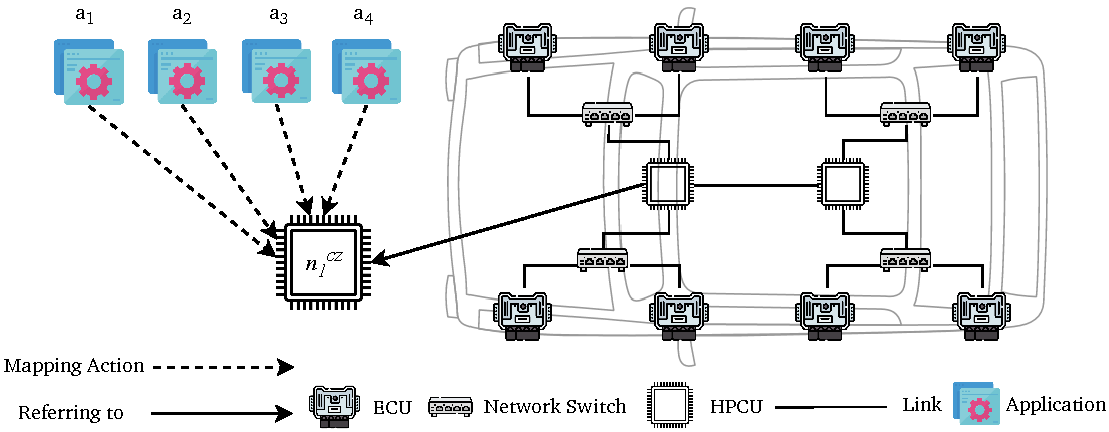
\includegraphics[width=1\columnwidth]{figures/mapping_action.pdf}
	\caption{A vehicle architecture including assignment of applications to an HPCU ($n_{1}^{cz}$).  
	}
	\label{mapping}
    \end{figure}

    \subsection{Mapping Action}
    Assigning applications, which consist of processes/threads, to control nodes such as ECUs or the cores of an HPCU is defined as a mapping action (see Figure \ref{mapping}), as explained as fundamental concepts in Chapter~\ref{basicConcepts}. To automate the mapping process, a mapping indication as $m_{ij}$ is considered in the system model comprising different sub-variables. It represents a possible assignment of different applications ($j$) to various control nodes ($i$)~\cite{askaripoor2023designer}. 
    According to the example presented in Figure~\ref{mapping}, assigning $a_4$ to $n_{1}^{cz}$ is denoted by ${m_{14}}.{a_4}^{n_{1}^{cz}}$ as a mapping variable. Moreover, the mapping variables of a thread belonging to an application that is set as a sender or a receiver are symbolized as ${m_{ij}}^{s}$ and ${m_{ij}}^{r}$, respectively. For example, the mapping variables of $t_1$ from $a_1$ as the sender running on $n_{1}^{cz}$, and $t_1$ from $a_4$ as the receiver executing on $n_{7}^{cz}$ are indicated with $m_{11}^{s}.{a_1}^{n_1^{cz}}$ and $m_{74}^{r}.{a_4}^{n_7^{cz}}$, respectively (refer to Figure~\ref{routing_rh_new}~(a)). Similarly, each $n_{i}^{cz}$ includes all mappings of existing applications, meaning that each $a_i$, which consists of a $t_i$ or multiple $t_i$, can be executed on each $n_{i}^{cz}$~\cite{askaripoor2023designer}.

    \subsection{Communication Message}

     Multiple variables are defined in the system model to create automatic message routings for a designed vehicle E/E architecture using the introduced computer-aided tool. A communication message is a piece of information sent from a sender to a receiver. In the specified model, a communication message $d_i$ is specified by a tuple $d_i$~$=$~\{$d_i.ch_i$,~$d_i.c_i$,~$d_i^{in}$,~$d_i^{out}$, $d_i.rt$, $d_i.el$\}. The message chain is characterized by $d_i.ch_i$, containing the threads, as the sender and receiver, and a communication task that transfers the communication message and constitutes the related application in a correct temporal order. Each $d_i$ includes a communication task, as described before, which carries the message symbolized with $d_i.c_i$.
    The message $d_i$ received by a node $n$ is represented as $d_i^{in}$ while $d_i^{out}$ designates the
    $d_i$ sent by the node $n$. Following the shown example in Figure~\ref{routing_rh_new}, the message chain $d_1.ch_1$ for $d_1$ consists of two threads related to applications $a_{1}$ and $a_{4}$ and a communication task $c_1$ (yellow dots in Figure~\ref{routing_rh_new}~(a) over the enumerated path) routing over five links in the visualized temporal order (yellow frames in Figure~\ref{routing_rh_new}~(b)). Note that each application thread can only generate one communication message, which is then transmitted via one communication task~\cite{askaripoor2023designer}. 

    In addition, the message $d_i$ sent out from $n_a$ over $l_{a,b}$ is denoted as $d_i^{out}.l_{a,b}^{n_a}$, whereas the message $d_i$ received by $n_a$ over $l_{b,a}$ is characterized as $d_i^{in}.l_{b,a}^{n_a}$ (refer to Table~\ref{notations}). The response time of a communication message is indicated by $d_i.rt$, which represents the time between the beginning of the period and the end of the last communication task. Meanwhile, the end-to-end latency $d_i.el$ represents the time between the start of the first task and the end of the last task~\cite{askaripoor2023designer}. The significance of these two parameters will be explained in the following sections.
        \begin{figure}[t!]
    	\centering
    	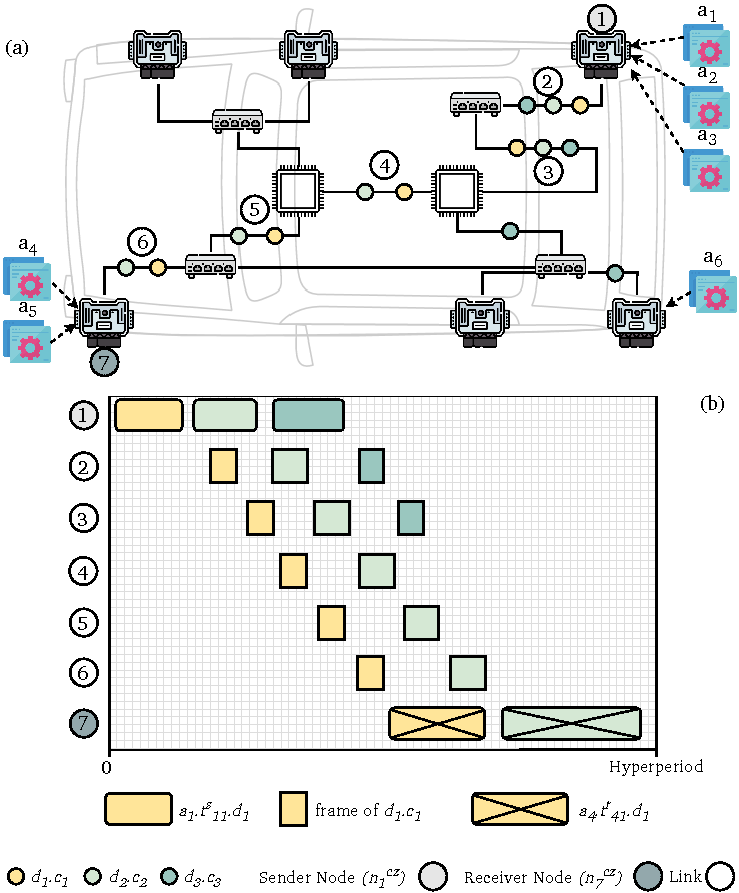
\includegraphics[width=0.98\columnwidth]{figures/schedules.pdf}
    	\caption{(a) A vehicle topology which shows generated paths for communication messages from senders to the receivers and mapped applications to the control nodes. Each colorful dot represents a communication task associated with a communication message. In this example, each application comprises a single application thread. (b) Calculated time-triggered schedules from the sender ($n_{1}^{cz}$) to the receiver ($n_{7}^{cz}$). It includes schedules for the sender (number one, with thread slots that are not crossed) and the receiver application threads (number seven, with thread slots that are crossed). The schedules of communications tasks (yellow and light green frames of the tasks in numbers two to six) over the generated path (only the enumerated route in (a)) are also included. The path routing two communication messages ($d_1$ and $d_2$) is considered. As can be seen, message dependency for the sender and receiver and path dependency for communication tasks are fulfilled. The representations for light green and dark green frames are similar to the yellow ones~\cite{askaripoor2023designer}.}
    	\label{routing_rh_new}
        \end{figure}
    
    \subsection{Application}
    
    An application $a_i$ is a collection of application threads that can act as senders or receivers of communication messages to perform a specific function. The application is defined by the tuple $a_i = \{a_i.t_{ij}, a_i.t_{ij}^{s}.d_i, a_i.t_{ij}^{r}.d_i\}$, where $a_i.t_{ij}$ includes one or multiple application threads $t_{ij} = \{t_{i1}, t_{i2}, ..., t_{ij}\}$, with $j \in \mathbb{N}$, indicating that each $a_i$ can have one or many $t$. Additionally, $a_i.t_{ij}^{s}.d_i$ represents the application thread $t_{j}$ belonging to $a_i$ that sends the communication message $d_i$, whereas $a_i.t_{ij}^{r}.d_i$ denotes the $t_{j}$ of $a_i$ that receives $d_i$, as stated in Table~\ref{notations}.


    \subsection{Timing Limitations}
    
    The current version of the proposed framework in this thesis offers a non-preemptive time-triggered scheduling scheme for all application threads running on the control nodes and routed communication tasks over the network links. As a result, some additional timing constraints have been incorporated into the system, similar to those presented in~\cite{zhang2014task}, which are explained below.
    
    \subsubsection{Serialization Delay}
    %When a thread completes its task, it takes some time before the data can be packed into frames and sent over the network. This time is denoted by \textit{sd}. 
    
    When an application thread completes its task, it takes some time before the data can be packed into frames and sent over the network. This time, often called the serialization delay, is crucial to overall system performance. In the system model, this time is denoted by \textit{sd}. 
    The serialization delay represents the time required to convert the processed data into a format suitable for transmission. In other words, it is the time it takes to serialize a packet, meaning how long it takes to physically put the packet on the wire. 
    During this stage, the data is typically transformed into a serialized representation, such as binary or JSON, allowing it to be efficiently transmitted across the network. The duration of the serialization delay can vary depending on factors such as the complexity of the data, the chosen serialization method, and the underlying hardware resources.
    It is worth noting that the network conditions and bandwidth limitations can influence the serialization delay. In scenarios where the available network bandwidth is constrained, the serialization delay may become more noticeable as the system waits for available network resources to transmit the serialized data. Considering these factors during system design and network provisioning is essential to ensure efficient data transfer~\cite{askaripoor2023designer}.

%It is important to consider the impact of the serialization delay when designing and optimizing networked systems. While the thread's task completion time may be minimal, the serialization delay can introduce additional latency and affect the overall responsiveness of the system. Therefore, it is crucial to analyze and optimize this aspect to minimize any potential bottlenecks and ensure efficient data transmission.
%Several techniques can be employed to mitigate the serialization delay. One approach is to utilize efficient serialization libraries or protocols that are specifically designed for high-performance data serialization. These libraries often provide optimizations such as data compression, binary serialization formats, and parallelization to reduce the time taken during serialization.
%Additionally, optimizing the underlying hardware infrastructure can also help reduce the serialization delay. This can involve utilizing faster processors, improving memory access patterns, or employing specialized hardware accelerators for serialization tasks. By leveraging hardware advancements, it becomes possible to decrease the time required for serialization, thereby enhancing the overall system throughput.
%In conclusion, the serialization delay (\textit{sd}) represents the time required to convert processed data into a format suitable for network transmission. Acknowledging its impact and employing optimization strategies can significantly enhance the overall system performance, reducing latency and improving data throughput in networked environments.


    \subsubsection{Deserialization Delay}
%Similarly, when a frame arrives at a control node, it requires a specific amount of time to be unpacked and processed before the relevant node can use the data. This time is referred to as \textit{rd}.

    When a frame arrives at a control node, it requires a specific amount of time to be unpacked and processed before the relevant node can effectively utilize the contained data. This time, commonly known as the deserialization delay and indicated as \textit{rd} in the framework's system model, plays a vital role in the overall efficiency and responsiveness of the system.
    This delay stands for the time needed to extract the serialized data from the received frame and convert it back into its original format. This process involves reversing the serialization process, which may comprise operations like decoding binary representations, parsing JSON structures, or reconstructing complex data objects. The duration of the deserialization delay can change due to various factors, such as the complexity of the data, the selected approach, and the computational resources available at the control node~\cite{askaripoor2023designer}.

%Understanding and managing the impact of the deserialization delay is crucial in optimizing system performance. Even if the frame arrives promptly, the deserialization delay can introduce additional processing time and potentially become a limiting factor in achieving real-time responsiveness. Therefore, it is essential to analyze and minimize this delay to ensure efficient data utilization and timely decision-making at the control node.

%Various techniques can be employed to mitigate the deserialization delay. Employing efficient deserialization libraries or protocols specifically designed for high-performance data reconstruction can significantly reduce the time required for this process. These libraries often offer optimizations such as parallel processing, caching mechanisms, or optimized algorithms tailored for rapid and accurate data extraction.

%Optimizing the computational resources at the control node is another critical aspect of minimizing the deserialization delay. This can involve utilizing faster processors, optimizing memory access patterns, or employing specialized hardware accelerators for deserialization tasks. By leveraging these hardware advancements, the time taken for data extraction can be reduced, enhancing the overall responsiveness of the system.

%It is important to note that network conditions and bandwidth limitations can also influence the deserialization delay. In scenarios where the available network bandwidth is limited, the deserialization delay may become more noticeable as the control node awaits the complete frame to initiate the deserialization process. Considering these factors during network design and provisioning can help ensure efficient and timely data processing.

%In conclusion, the deserialization delay (\textit{rd}) represents the time required to extract and process serialized data upon the arrival of a frame at a control node. Recognizing its impact and implementing optimization strategies can significantly enhance system efficiency, reducing processing latency, and enabling timely utilization of the received data at the control node.

    \subsubsection{Processing Delay}

%The maximum processing delay of a communication frame in a networking node is represented as \textit{pd}. It is defined as the time between the reception of the last bit on the input port and the earliest possible transmission of the first bit on the output port.

    The maximum processing delay of a communication frame in a networking node is a crucial metric that characterizes the time required for the node to process and forward the received frame. It signifies the delay from when the last bit of the frame is received on the input port until the earliest possible transmission of the first bit on the output port. This delay is represented as \textit{pd}.
    The processing delay encompasses various stages of frame handling within the networking node. Once the frame is received, it undergoes several essential operations, including header parsing, routing table lookup, potential payload processing, and potential modifications or encapsulations before being transmitted to the next destination. Each of these operations contributes to the overall processing delay. This delay can be influenced by factors such as the frame's complexity, the computational resources available in the node, and the network traffic load. For the complex frames or resource-constrained nodes, the processing delay may be longer, potentially leading to increased latency in the network. Therefore, it is essential to consider these factors during network design and provisioning to ensure that the processing delay remains within acceptable limits~\cite{askaripoor2023designer}.

%Efficient management of the processing delay is vital to ensure smooth and timely communication within the network. Minimizing this delay helps maintain low latency and enables fast data forwarding, which is particularly critical in real-time or high-performance network applications.
%To reduce the processing delay, networking nodes employ various optimization techniques. These include hardware acceleration, specialized routing algorithms, efficient lookup tables, and parallel processing architectures. By leveraging these techniques, nodes can perform the necessary tasks swiftly and effectively, minimizing the time spent in the processing stage.

%It's worth noting that while minimizing the processing delay is crucial, it should not compromise the accuracy or integrity of the frame processing. The networking node must accurately perform all necessary tasks, such as verifying the frame's integrity, ensuring security measures, and adhering to any required protocol specifications. Balancing speed and accuracy is key to achieving optimal performance while maintaining data reliability.

%In summary, the maximum processing delay (\textit{pd}) of a communication frame in a networking node represents the time required for the node to process and forward the received frame. By employing optimization techniques, considering network load, and ensuring accuracy in frame processing, the processing delay can be minimized, leading to low latency and efficient data transmission within the network.


    \subsubsection{Interpacket Gap}

%Additionally, we consider the interpacket gap, or \textit{ipg}, which is the required time between network packets or frames. This gap is necessary as a brief recovery time to allow devices to prepare for the reception of the next packet. 

    The interpacket gap indicated as \textit{ipg}, is considered, which represents the required time interval between consecutive network packets or frames. The interpacket gap serves as a crucial recovery period that allows network devices to prepare for the reception of the next packet.

    The purpose of the interpacket gap is to ensure proper synchronization and coordination between transmitting and receiving devices within a network. It allows devices to handle the processing and forwarding of the received packet, update internal states, and make necessary preparations before the arrival of the subsequent packet. This recovery time is critical in high-speed or heavily loaded networks, where devices require a momentary pause to avoid congestion, buffer overflows, or potential data loss.
    The duration of the \textit{ipg} is typically defined by network protocols or standards and can be different based on the specific requirements of the network environment. It may be specified in terms of time, e.g., microseconds or milliseconds, or as a multiple of the packet transmission time. The duration of this gap should be carefully chosen to strike a balance between efficient data transmission and allowing sufficient recovery time for network devices. Properly setting and managing the \textit{ipg} can significantly impact network performance and reliability. If the gap is too short, devices may not have enough time to process and prepare for the next packet, leading to increased packet loss, errors, or degraded performance. On the other hand, an excessively long \textit{ipg} can result in reduced network throughput and underutilization of available bandwidth~\cite{askaripoor2023designer}.

    Network administrators and engineers often fine-tune the \textit{ipg} based on the network infrastructure's specific characteristics and the traffic's nature. They consider factors such as network speed, latency, device capabilities, and the presence of other network optimization techniques like flow control or congestion avoidance algorithms.

%It's worth noting that the interpacket gap can also be influenced by external factors such as network congestion, transmission errors, or the presence of other network traffic. In such cases, dynamic adjustments or adaptive mechanisms may be employed to optimize the interpacket gap dynamically and ensure efficient network operation.

%In conclusion, the interpacket gap (\textit{ipg}) represents the necessary time interval between network packets or frames, allowing devices to recover and prepare for the reception of the next packet. Properly setting and managing the interpacket gap is crucial in maintaining network performance, avoiding congestion, and ensuring reliable data transmission in diverse network environments.

    \subsubsection{Bandwidth}

%Finally, the bandwidth is indicated by \textit{bw}, which represents the maximum possible amount of data transfer between two points of a network over the link in a specific time.


    Finally, the bandwidth, denoted by \textit{bw}, is a fundamental metric that characterizes the maximum potential data transfer rate between two points in a network over a specific link within a given time frame. It plays a crucial role in determining a network connection's overall capacity and performance.

    Bandwidth, typically measured in bits per second (bps), represents the amount of data that can be transmitted within a specified time duration. It limits the rate at which information can be exchanged between network devices, such as routers, gateways, switches, or communication links. The higher the bandwidth, the greater the volume of data that can be transferred in a given time, leading to faster and more efficient communication. \textit{bw} can be affected by the underlying infrastructure and technology used in the network. Factors such as cable quality, transmission medium (e.g., copper or fiber optic), and network equipment capabilities influence the achievable bandwidth for wired connections. In wireless networks, variables such as spectrum availability, modulation techniques, signal strength, and interference impact the available bandwidth.
    Various techniques are employed to make the most efficient use of available bandwidth. Network protocols and algorithms implement strategies such as congestion control, QoS mechanisms, and traffic prioritization to optimize data transfer and ensure fair sharing of network resources~\cite{askaripoor2023designer}.


%Understanding the available bandwidth is essential for network design, planning, and optimization. It allows network administrators and engineers to allocate resources effectively, ensure sufficient capacity to accommodate data traffic, and prevent congestion or bottlenecks that can degrade network performance.


%It is important to note that the effective bandwidth experienced by users may be lower than the theoretical maximum due to factors such as network congestion, latency, and protocol overhead. Real-world conditions and network traffic fluctuations can impact the actual data transfer rate, necessitating thorough monitoring, analysis, and capacity planning to deliver optimal performance.

%In summary, bandwidth (\textit{bw}) represents the maximum achievable data transfer rate between two points in a network over a specific link within a given time. It serves as a critical metric for network design, optimization, and resource allocation, enabling efficient communication and ensuring optimal performance in diverse networking environments.







    \section{Constraints MIP Formulation}\label{constraintformul}
    The E/E Designer framework creates automated mapping and automatic message routings. It considers path and message dependencies and calculates the time-triggered schedules for different application threads and communication tasks $c_i$ for a modeled vehicle E/E system. These threads run on various control nodes $n_{i}^{cz}$, and the communication tasks route over the network. The framework takes predefined boundary and optimization objectives into account. The E/E architecture presented in Figure~\ref{routing_rh_new} is characterized as a distributed system. This is done to proceed with the E/E Designer goals using a set of constraints.
    
    \subsection{Automated Mapping}
    To automatically assign applications, including their threads, to control nodes, the following constraint set is formulated: \newline
    	
    	$\forall i, j, k \in \mathbb{N}$,~${m_{ij}}$,~${m_{ik}}$,~${m_{ij}^{s}}$,~$m_{ij}^{r}$~$\in\mathcal{M} $, ${a_j}$, ${a_k}$, ${a_o}$, ${a_p}$, $a^{sc}$, $a^{asil_D}$, $a^{non-asil_D}$~$\in\mathcal{A}$, ${n_{i}^{cz}}$  $\in \mathcal{N}$:\newline
    	    
     $\textbf{if}$ $a_j$ $\notin$ $a^{sc}$ $\textbf{then}$\newline	
    \begin{equation}
    	%\boldmath
    	\sum_{i \in \mathbb{N}} {m_{ij}}.{a_j}^{n_{i}^{cz}} =1
    	\label{eq1}
    	%   \unboldmath
    \end{equation}
    
    
    	%	$\forall i, j$, ${m_i}$~$\in\mathcal{M} $, ${a_j}$~$\in\mathcal{A}$, ${n_{i}^{cz}}$  $\in N$:\newline
    
    
    \begin{equation}
    	%\boldmath
    	%\sum_{m_s=(A_{sen}, N_s) \in m, m\in M } m_{s}=1	
    	%i, j \in \mathbb{N} 
    	%\sum_{j \in \mathbb{N}} {m_{ij}}.{n_i^{cz}}.a_j \geq{1}
    	\sum_{j \in \mathbb{N}} {m_{ij}}.{a_j}^{n_{i}^{cz}} \geq{1}
    	\label{eq2}
    	%   \unboldmath
    \end{equation}	
    	
    \begin{equation}
    	%\boldmath
    	%\sum_{m_s=(A_{sen}, N_s) \in m, m\in M } m_{s}=1	
    	%i, j \in \mathbb{N} 
    	 {m_{ij}^{s}}.{a_j}^{n_{i}^{cz}} + {m_{ik}^{r}}.{a_{k}}^{n_{i}^{cz}}\leq{1}
    	\label{eq3}
    	%   \unboldmath
    \end{equation}	
    
    
    $\textbf{if}$ $a_k$ $\in$ $a^{sc}$ $\textbf{then}$\newline	
    \begin{equation}	
    	%\boldmath
    	%\sum_{m_s=(A_{sen}, N_s) \in m, m\in M } m_{s}=1	
    	\sum_{i \in \mathbb{N} } {m_{ik}}.{a_{k}}^{n_{i}^{cz}} =2
    	\label{eq4}
    	%   \unboldmath
    \end{equation}
    	
    \begin{equation}
    	%\boldmath
    	%\sum_{m_s=(A_{sen}, N_s) \in m, m\in M } m_{s}=1	
    	%i, j \in \mathbb{N} 
    	{m_{ij}}.{a_j}^{n_{i}^{cz}} + {m_{ik}}.{a_{k}}^{n_{i}^{cz}}\leq{1}
    	\label{eq5}
    	%   \unboldmath
    \end{equation}		
    \vspace{1pt}
    
    $\textbf{if}$ $a_o$ $\in$ $a^{asil_D}$ $\textbf{and}$ $a_p$ $\in$ $a^{non-asil_D}$ $\textbf{then}$\newline	
    %$\textbf{if}$ $a_p$ $\in$ $a^{sc}$ $\textbf{then}$\newline	
    
    \begin{equation}
    	%\boldmath
    	%\sum_{m_s=(A_{sen}, N_s) \in m, m\in M } m_{s}=1	
    	%i, j \in \mathbb{N} 
    	{m_{io}}.{a_o}^{n_{i}^{cz}} + {m_{ip}}.{a_{p}}^{n_{i}^{cz}}\leq{1}.
    	\label{eqffi6}
    	%   \unboldmath
    \end{equation}
    
    
    %proofread
    The condition (\ref{eq1}) ensures that each application is only mapped once on each ${n_{i}^{cz}}$. Moreover, to distribute the applications, including their threads, to all existing control nodes, 
    each ${n_{i}^{cz}}$ must execute at least one application ($a_j$) which is encoded in Eq. (\ref{eq2}). Based on the constraint (\ref{eq3}), the sender and receiver threads from two different applications, transferring a communication message, cannot be executed on the same control node~\cite{askaripoor2023designer}. 
    \subsubsection{Redundancy in Mapping}
    To meet the redundancy requirement following ISO 26262~\cite{iso26262}, the safety-critical applications $a^{sc}$ set must be run redundantly. Hence, condition (\ref{eq4}) forces each $a^{sc}$ to be executed twice on various $n_{i}^{cz}$~\cite{askaripoor2023designer,askaripoor2022architecture}. 
    \subsubsection{FFI in Mapping}
    In addition, to fulfill the FFI demand for $a^{sc}$ and $a^{asil}$, non-safety $a_j$ and safety-critical $a_{k}$ applications must not be run on the same $n_{i}^{cz}$ which is formulated in (\ref{eq5}). Similarly, to provide FFI condition during the automated mapping process for ASIL D applications, constraint (\ref{eqffi6}) is stated. Based on (\ref{eqffi6}), ASIL D and non-ASIL D applications cannot be executed on the same control node~\cite{askaripoor2022architecture,askaripoor2023designer}.
      The sets of all mapping variables are defined as $\mathcal{M}$ and all applications, including safety-critical ones, as $\mathcal{A}$. Note that all mapping variables are specified as binary variables (i.e., 0 or 1). The same constraints are applied for each core of an HPCU ($n^{cz_c}$). That is, the redundancy and FFI conditions are valid for various cores with different ASIL levels.   %\newline
    
    

  
    %\subsection{Environmental ECU}
    
    \subsection{Automatic Message Routing}
    
    Message routing plays a pivotal role in automotive networks, where many nodes, comprising ECUs, HPCUs, switches, and gateways, collaborate to ensure smooth vehicle operations. As modern automobiles become increasingly sophisticated, incorporating various functionalities and advanced systems, efficient and reliable message routing becomes paramount.
    In automotive networks, messages flow between nodes to exchange vital information about engine control, transmission, braking, safety systems, entertainment, and more. These messages typically follow predetermined protocols and data formats, such as the CAN, time-triggered CAN, FlexRay, LIN, and Ethernet, to ensure compatibility and interoperability across the network.
    The primary goal of message routing is to deliver messages from their source nodes to their intended destinations, optimizing the data transmission process while adhering to the network's constraints. Several factors influence the routing decisions within automotive networks, including the message's priority and criticality, the available bandwidth, the network topology, and the characteristics of the nodes involved, as illustrated in Chapter~\ref{basicConcepts}.
    
    
    
    The presented model-based framework proposes automatic message routing for modeled E/E systems, including single, multicast, redundant, and homogeneous redundant paths. In the following, each of these routes is explained and encoded.
    
    \begin{figure}[t]
    	\centering
    	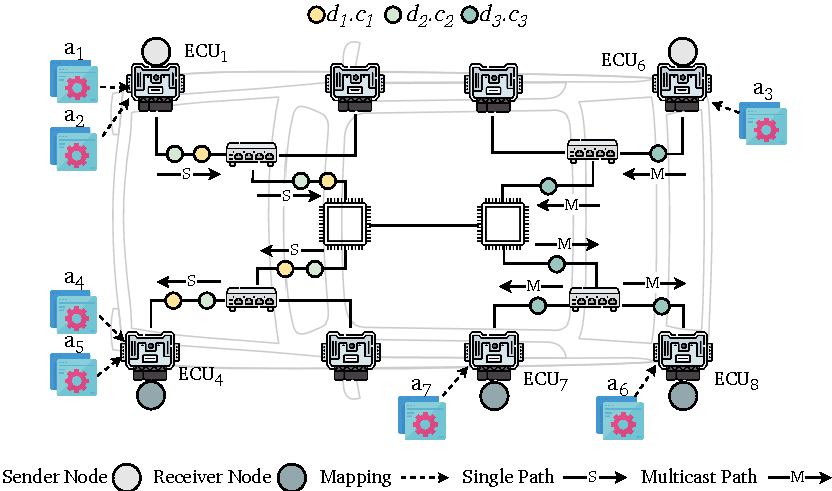
\includegraphics[width=1\columnwidth]{figures/s_routing.pdf}
    	\caption{A vehicle architecture comprising intermediate and control nodes, links, and assigned applications to ECUs. A single (arrows with S) and a multicast (arrows with M) paths are generated in order to send communication messages (colored dots), created by applications, from sender nodes to receiver nodes.  
    	}
    	\label{routing_sm}
    \end{figure}
    
    \subsubsection{Single Routing}
    
    %Our previous work~\cite{9565115} presented all the constraints required to automatically create network message routing, including single, redundant, and HR routings. HR routes are backup paths in a network that are identical in terms of capacity, topology, and performance to the primary path. Therefore, they are disjoint. HR routes are typically implemented to provide high availability and fault tolerance for critical applications and services.On the other hand, redundant routes refer to the presence of any backup or alternative paths in a network. They are not necessarily disjoint. The main goal of redundant routes is to ensure network availability and reduce downtime in the event of a failure.
    
    %In the \textit{E/E Designer}, we use similar constraints to our previous work to create routes but with changes regarding multicast routing, automated mapping, and the joint constraint set. These changes affect the entire routing system model. However, only changes related to multicast paths will be explained in the following.\newline  
    
    Single routing, also known as unicast routing, involves the transmission of a message from a source control node to a single destination control node (see Figure~\ref{routing_sm}).
    In this type of routing, each message is addressed to a specific destination node, and the routing process focuses on finding the optimal path to deliver the communication message to that particular node. Single routing is commonly used for point-to-point communication, where a message is intended for a specific recipient~\cite{9565115}.
    The routing decisions are typically based on various factors such as network topology, available bandwidth, latency requirements, cost, and reliability, which will be illustrated in the following sections. 
    
    In Figure~\ref{routing_sm}, a single path (indicated as S) is shown to transmit two communication messages ($d_1$ and $d_2$) from their senders to their receivers— yellow and light green dots in the Figure~\ref{routing_sm} represent two communication tasks belonging to two communication messages routed over the network's links. 
    
    Considering the previous work~\cite{9565115}, the following constraints are utilized to encode the single message routing:\newline
    
    	
    
    $\forall i, j, k$, ${n_{j}}$  $\in \mathcal{N}$, $d_k^{in},~d_k^{out}\in~\mathcal{D}$, ${m_{ij}}^{s}$, $m_{ij}^{r}$~$\in\mathcal{M} $:\newline

	\begin{equation}
		%m_s - m_d -\sum_{d_{out} \in d} d_{out} \leq 0
		 {m_{ij}^{s}} - m_{ij}^{r} - \sum_{j \in \mathbb{N} } n_{j}.d_{k}^{out} \leq 0 
		\label{eqs3} 
		%\unboldmath
	\end{equation}
	
	\begin{equation}%\boldmath
		%m_s +\sum_{d_{in} \in d } d_{in}<=1
		{m_{ij}^{s}}  + \sum_{j \in \mathbb{N} } n_{j}.d_{k}^{in} \leq 1 
		\label{eqs4}
	\end{equation}
	
	\begin{equation}%\boldmath
		%m_d - m_s -\sum_{d_{in} \in d} d_{in}<=0
		{m_{ij}^{r}} - m_{ij}^{s} - \sum_{j \in \mathbb{N} } n_{j}.d_{k}^{in} \leq 0
		\label{eqs5}
	\end{equation}

	\begin{equation}%\boldmath
		%m_d +\sum_{d_{out} \in d} d_{out}<=1
		{m_{ij}^{r}}  + \sum_{j \in \mathbb{N} } n_{j}.d_{k}^{out} \leq 1 
		\label{eqs6}
	\end{equation}
	

	\begin{equation}%\boldmath
		%m_s - m_d +\sum_{d_{in} \in d} d_{in} - \sum_{d_{out} \in d} d_{out} = 0
		{m_{ij}^{s}} - m_{ij}^{r} + \sum_{j \in \mathbb{N} } n_{j}.d_{k}^{in} - \sum_{j \in \mathbb{N} } n_{j}.d_{k}^{out} = 0.
		\label{eqs7}
	\end{equation}
	



    %proofread
	%Based on the constraint \eqref{eqs3}, at least one out-going communication message ($d_i^{out})$ over a link must exist for a sender node (i.e., when in the automated mapping, mapping variable $m_{ij}^{s} = 1$ relevant to $n_j$). This condition does not have any impact in the routing process when the node is not a sender. In (\ref{eqs4}), a sender node ($n_j$) is forced to block all in-coming communication messages ($d_i^{in}$), related to $d_i$, which are coming from the other nodes. This fulfills no activated $d_i^{in}$ for the node ($n_j$) which is a sender meaning that $m_{ij}^{s} =1$ and $m_{ij}^{r} =0$. For example, in figure~\ref{routing_sm}, $ECU_1$, as a sender, has only one activated $d_i^{out}$ and no triggered $d_i^{in}$ to route a message to the next node.  
	
	Based on constraint \eqref{eqs3}, there must be at least one outgoing communication message ($d_k^{out}$) over a link for a sender node. This constraint applies when the automated mapping assigns a mapping variable $m_{ij}^{s}$ equal to 1 for the sender node $n_j$. However, this condition does not affect the routing process when the node is not a sender.
    In Eq.~\eqref{eqs4}, a sender node $n_j$ is required to block all incoming communication messages ($d_k^{in}$) related to $d_k$ that are coming from other nodes. This ensures that no activated $d_k^{in}$ messages exist for the sender node $n_j$, which means that $m_{ij}^{s} = 1$ and $m_{ij}^{r} = 0$. For example, in Figure~\ref{routing_sm}, the sender node $ECU_1$ has only one activated $d_k^{out}$ and no triggered $d_k^{in}$ to route communication messages to the next node. 
	
	
	Similarly to condition \eqref{eqs3}, but this time for a node ($n_j$) as a receiver ($m_{ij}^{s} =0$ and $m_{ij}^{r} =1$) of a communication message, at least one incoming message ($d_k^{in}$) over a link must be set, according to Eq. \eqref{eqs5}. Also, constraint \eqref{eqs6} expresses that the receiver node must not have any triggered outgoing data ($d_k^{out}$). In Figure~\ref{routing_sm}, there is only one activated $d_k^{in}$ and no $d_k^{out}$ for $ECU_4$ as a receiver to create a single route.
	%Considering \eqref{eqs3} and \eqref{eqs4}, the sender and receiver can have more than one $d_i^{out}$ and $d_i^{in}$, respectively. Therefore, forcing the sender and receiver nodes to have only one triggered outgoing and incoming communication messages, respectively, to create a single path, is met by applying \eqref{eqs7}. Furthermore, the same condition enforces intermediate nodes, which are neither sender nor receiver of a message, to either have no triggered message or to have exactly one activated incoming message ($d_i^{in}$) and one triggered outgoing message ($d_i^{in}$). 
	Considering Eqs. \eqref{eqs3} and \eqref{eqs4}, it is possible for the sender and receiver to have multiple $d_k^{out}$ and $d_k^{in}$ values, respectively. Therefore, to create a single path, it is necessary to ensure that the sender and receiver nodes have only one triggered outgoing and incoming communication message, respectively, as stated in Eq. \eqref{eqs7}. Furthermore, this condition applies to intermediate nodes that are neither senders nor receivers of a message. These intermediate nodes must either have no triggered message or have exactly one activated incoming message ($d_k^{in}$) and one triggered outgoing message ($d_k^{in}$). 
	
	
  
	
	
	%In order to connect the $d_i^{in}$ to the $d_{out}$ while both nodes are connected by a directed link, the constraint \eqref{eq8} is used. For instance, if the $d_{out}$ routing out from $N_1$, as the starting point of link $\vec{L_1}$, over the link $\vec{L_1}$ becomes activated, the $d_{in}$ routing into $N_2$, as the finishing point of the link $\vec{L_1}$, over the link $\vec{L_1}$ must be activated too in respect of \eqref{eq8}.
	
	
	%Constraint \eqref{eqs7} consists of several explanations. If a node gets allocated for $A_{sen}$ as well as $A_{rec}$ simultaneously, so that the node becomes a source and a destination, it must not comprise any activated data ($d_{in}, d_{out}$) according to \eqref{eqs7}, while drawing attention to constraints \eqref{eq4},\eqref{eq6} as well. 
	
	%The source node, in the event of running an $A_{sen}$ on an arbitrary node ($N_s \Rightarrow{m_s=1}$), is obliged to block all in-coming data ($d_{in}$) which are coming from the other nodes, according to constraint \eqref{eq4}; as a result, there is no $d_{in}$ for the relevant node. 
	
	%Similarly to \eqref{eq3}, but this time for a node as the destination ($N_d \Rightarrow{m_d=1}$), at least one in-coming datum ($d_{in}$) over a link must be applied, according to constraint \eqref{eq5}. Constraint \eqref{eq6} expresses that the destination must not have any activated out-going data ($d_{out}$); in other words, if $(N_d \Rightarrow{m_d=1}) \Rightarrow{\sum d_{out}=0}$. 
	
	
	%Constraint \eqref{eq7} consists of several explanations. If a node gets allocated for $A_{sen}$ as well as $A_{rec}$ simultaneously, so that the node becomes a source and a destination, it must not comprise any activated data ($d_{in}, d_{out}$) according to \eqref{eq7}, while drawing attention to constraints \eqref{eq4},\eqref{eq6} as well. 
	
	
	%Moreover, a node, allocated as the source not the destination (i.e., $m_s=1, m_d=0$), must have exactly one activated out-going datum ($d_{out}$) in respect of \eqref{eq7}. While, a node, assigned to $A_{rec}$, must include exactly one triggered in-coming datum (i.e., $\sum d_{in}=1$) w.r.t. constraint \eqref{eq7}. In addition, based on \eqref{eq7}, the nodes are enforced, which are neither a source nor a destination for routing a unique datum, to either have no triggered data (i.e., $\sum d_{out}=0 , \sum d_{in}=0$) or to have precisely one activated in-coming datum and one activated out-going datum (i.e., $\sum d_{out}=1, \sum d_{in}=1$). These constraints encode single routings while avoiding routing cycles. In order to connect the $d_{in}$ to the $d_{out}$ while both nodes are connected by a directed link, the constraint \eqref{eq8} is used. For instance, if the $d_{out}$ routing out from $N_1$, as the starting point of link $\vec{L_1}$, over the link $\vec{L_1}$ becomes activated, the $d_{in}$ routing into $N_2$, as the finishing point of the link $\vec{L_1}$, over the link $\vec{L_1}$ must be activated too in respect of \eqref{eq8}. The same concept is applied for $\vec{L_2}$.\newline


    \subsubsection{Multicast Routing}\label{multicastrouting}

    Multicast routing involves the transmission of a message from a source node to multiple destination nodes simultaneously. In this type of routing, a single message is addressed to a group of destination nodes rather than a specific node.
    The routing process aims to replicate the message and deliver it to all the nodes in the multicast group efficiently.
    %The routing decisions in multicast routing are typically based on factors such as group membership, group addressing, and network efficiency.
    It is commonly used for applications where the same information needs to be sent to multiple recipients, such as video streaming, software updates, and distributed simulations. A multicast path (indicated by the arrow visualized with M) is shown in Figure~\ref{routing_sm} for transmitting the $d_3$ message from $ECU_6$ to two receivers, namely $ECU_7$ and $ECU_8$. The E/E Designer uses the following conditions to automatically create multicast routes for the designed automotive networks~\cite{askaripoor2023designer}.
     \newline


%$\forall i, j, a, b$, ${n_{j}}$, ${n_a}$, ${n_b}$  $\in \mathcal{N}$, $l_{a,b}$, $l_{b,a}$ $\in \mathcal{L}$, $d_i^{in},~d_i^{out}\in~\mathcal{D}$, ${m_{ij}}^{s}$, $m_{ij}^{r}$~$\in\mathcal{M} $:\newline


    $\forall i, j, k$, ${n_{j}}$  $\in \mathcal{N}$, $d_k^{in},~d_k^{out}\in~\mathcal{D}$, ${m_{ij}}^{s}$, $m_{ij}^{r}$~$\in\mathcal{M} $:\newline

	\begin{equation}
		%m_s - m_d -\sum_{d_{out} \in d} d_{out} \leq 0
		 {m_{ij}^{s}} \times ({m_{ij}^{s}} - m_{ij}^{r}) - {m_{ij}^{s}} \times \sum_{j \in \mathbb{N} } n_{j}.d_{k}^{out} \leq 0 
		\label{eqm1} 
		%\unboldmath
	\end{equation}
	
	\begin{equation}%\boldmath
		%m_s +\sum_{d_{in} \in d } d_{in}<=1
		 {m_{ij}^{s}} \times \sum_{j \in \mathbb{N} } n_{j}.d_{k}^{in} \leq 0 
		\label{eqm2}
	\end{equation}
	
	\begin{equation}%\boldmath
		%m_d - m_s -\sum_{d_{in} \in d} d_{in}<=0
		{m_{ij}^{r}} \times ({m_{ij}^{r}}  - m_{ij}^{s})  - {m_{ij}^{r}} \times \sum_{j \in \mathbb{N} } n_{j}.d_{k}^{in} = 0
		\label{eqm3}
	\end{equation}

	\begin{equation}%\boldmath
		%m_d +\sum_{d_{out} \in d} d_{out}<=1
		 {m_{ij}^{r}} \times \sum_{j \in \mathbb{N} } n_{j}.d_{k}^{out} \leq 0 
		\label{eqm4}
	\end{equation}
	



    \begin{equation}	
    	%\boldmath
    	%\sum_{m_s=(A_{sen}, N_s) \in m, m\in M } m_{s}=1	
    	\sum_{j \in \mathbb{N} } n_{j}.d_k^{out} - \sum_{j \in \mathbb{N} } n_{j}.d_k^{in}  = {m_{ij}^{s}} - m_{ij}^{r}
    	\label{eqm5}
    	%   \unboldmath
    \end{equation}
    \; \; \; \; \; \; \; \; \; \; \; \; \; \; \; \; \; \; \; \; \; \; \; \; \; \; \; \; \; \;\; \; \; \; \; \;or
    \begin{equation*}
    	\begin{split}
    	\sum_{j \in \mathbb{N} } n_{j}.d_k^{out} \geq {m_{ij}^{s}} - m_{ij}^{r} + \sum_{j \in \mathbb{N} } n_{j}.d_k^{in}.
    	\label{eqm6}
    	%\unboldmath
    	\end{split}		
    \end{equation*}


     Constraint \eqref{eqm1} reveals that at least one outgoing communication message ($d_k^{out}$) over a link must be activated for a sender node. This rule is triggered for the sender node, i.e., $m_{ij}^{s}$ equal to 1 for the sender node $n_j$, as each variable of the Eq.~\eqref{eqm1} is multiplied by $m_{ij}^{s}$. Moreover, a sender node cannot have any activated communication message coming into the sender from other nodes, according to Eq. \eqref{eqm2}. 
     As a receiver, a node must comprise precisely one triggered inflowing message ($d_k^{in}$) to fulfill requirements for generating multicast paths (refer to Eq. \eqref{eqm3}). Considering the multiplication terms, this condition is only valid for the receiver nodes.
     Furthermore, a receiver must inhibit all outgoing communication messages ($d_k^{out}$) related to $d_k$ that are coming from other nodes, based on constraint \eqref{eqm4}. This guarantees that no initiated $d_k^{out}$ messages exist for the receiver node $n_j$. 
     
     According to Eq. \eqref{eqm5}, the intermediate nodes must either have an equal number of incoming and outgoing communication messages or the number of $d_k^{out}$ messages must be greater than equal to $d_k^{in}$ messages. This condition enforces the intermediate nodes to include either one input and one output or one input and multiple outputs to meet the multicast routing requirements. In Figure~\ref{routing_sm}, considering the multicast path, the network switch has only one entering message or $d_k^{in}$ and two departing messages ($d_k^{out}$) to receivers $ECU_7$ and $ECU_8$.   
     

	
    \subsubsection{Redundant Routing}
    
     It plays an essential role in ensuring reliable and fault-tolerant communication in automotive communication networks between various nodes, such as control and networking nodes in vehicles. As automotive systems become increasingly complex and interconnected, redundancy becomes essential to maintain system functionality and safety, especially for mixed-critical systems.  
    This type of routing involves the provision of multiple communication paths between nodes, allowing for alternate routes in case of link failures, congestion, or other communication disruptions. These redundant paths serve as backups in case of link failures or congestion. The redundant paths in physical routes, protocols, or transmission media may differ. This redundancy enhances the robustness and resilience of the network, minimizing the risk of communication failures and providing backup options in case of any unforeseen issues.
    One approach to implementing redundant routing is the use of parallel communication channels. Multiple physical or virtual links between nodes, e.g., ECUs, can be established, allowing for simultaneous data transmission over different paths. If one link experiences a failure or degradation, the system can automatically switch to an alternate path, ensuring uninterrupted communication. This redundancy helps to mitigate the impact of single-point failures and enhances the overall reliability of the network~\cite{iso26262, smirnov2018automatic, 9565115, askaripoor2023designer}. 
    
    The E/E Designer framework creates redundant physical paths for safety-critical applications to transmit critical communication messages. Redundant routings are not necessarily disjoint, meaning they may share common nodes or links between senders and receivers. For example, in Figure~\ref{routing_rh}, there is one redundant path for the communication message, $d_1$, from $ECU_1$ to $ECU_4$. This route transmits an additional communication task ($c_1$) belonging to a communication message ($d_1$) (it is shown with a yellow dot with a red border) from the sender to the receiver. This routing is not disjoint as it shares two network switches with the other related to $d_1$. The set of constraints below is integrated into the framework's system model to generate automatic redundant routing. \newline  
    
    % technique employed in redundant routing is the use of diverse routing protocols. Different routing algorithms or strategies can be utilized to compute alternate paths between ECUs. These protocols take into account factors such as link quality, traffic load, and network topology to dynamically select the optimal route for data transmission. By diversifying the routing protocols, the network can adapt to changing conditions and avoid common-mode failures that can affect a single routing algorithm.
    
    %Redundant routing in automotive communication networks also involves monitoring and detection mechanisms. Continuous monitoring of link status, bandwidth utilization, and other network metrics enables proactive identification of potential failures or congestion. With real-time information, the system can trigger automatic rerouting or load balancing to redistribute traffic and avoid bottlenecks. Additionally, fault detection mechanisms can detect link failures or communication errors and initiate rapid recovery actions, such as activating redundant paths or notifying the appropriate ECUs for corrective measures.
    
    %Overall, redundant routing in automotive communication networks is essential for ensuring reliable and resilient communication among ECUs. It enhances system availability, fault tolerance, and safety, enabling efficient and uninterrupted data exchange in the increasingly complex automotive ecosystem. By leveraging redundant routing strategies, automotive systems can maintain high levels of performance and mitigate the impact of potential failures or disruptions, contributing to the overall reliability and robustness of modern vehicles.
     
        \begin{figure}[t]
    	\centering
    	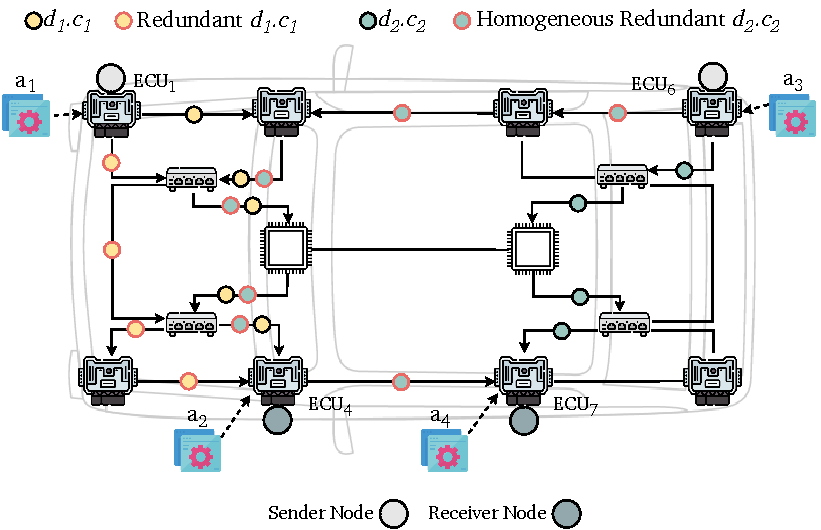
\includegraphics[width=1\columnwidth]{figures/hr_routing.pdf}
    	\caption{A modeled car architecture comprising intermediate and control nodes, links, and assigned applications to ECUs. A redundant (yellow dot with red border line) and a homogeneous redundant (green dot with red border line) routes are created in order to send communication messages (colored dots), created by applications, from sender nodes to receiver nodes.  
    	}
    	\label{routing_rh}
    \end{figure}
    
  
    
    
    $\forall i, j, k$, ${n_{j}}$  $\in \mathcal{N}$, $d_k^{in},~d_k^{out}\in~\mathcal{D}$, ${m_{ij}}^{s}$, $m_{ij}^{r}$~$\in\mathcal{M} $:\newline

	\begin{equation}
		%m_s - m_d -\sum_{d_{out} \in d} d_{out} \leq 0
		 {m_{ij}^{s}} - m_{ij}^{r} -  \sum_{j \in \mathbb{N} } n_{j}.d_{k}^{out} \leq -1 \times {m_{ij}^{s}}
		\label{eqr1} 
		%\unboldmath
	\end{equation}
	
	\begin{equation}%\boldmath
		%m_s +\sum_{d_{in} \in d } d_{in}<=1
		 {m_{ij}^{s}} \times \sum_{j \in \mathbb{N} } n_{j}.d_{k}^{in} \leq 0 
		\label{eqr2}
	\end{equation}
	
	\begin{equation}%\boldmath
		%m_d - m_s -\sum_{d_{in} \in d} d_{in}<=0
		{m_{ij}^{r}}  - m_{ij}^{s}  - \sum_{j \in \mathbb{N} } n_{j}.d_{k}^{in} \leq -1 \times {m_{ij}^{r}}
		\label{eqr3}
	\end{equation}

	\begin{equation}%\boldmath
		%m_d +\sum_{d_{out} \in d} d_{out}<=1
		 {m_{ij}^{r}} \times \sum_{j \in \mathbb{N} } n_{j}.d_{k}^{out} \leq 0 
		\label{eqr4}
	\end{equation}
	


    \begin{equation}
    	  2 \times {m_{ij}^{d}} - 2 \times m_{ij}^{s} - \sum_{j \in \mathbb{N} } n_{j}.d_k^{in} + \sum_{j \in \mathbb{N} } n_{j}.d_k^{out} = 0.
    	\label{eqr5}
    	%\unboldmath
    \end{equation}\newline
    
    
    
 
    Constraint \eqref{eqr1} illustrates that a sender node must activate at least two outgoing communication messages ($d_k^{out}$) over a link. This requirement is applied to the sender node; in other words, when the mapping variable, $m_{ij}^{s}$, has a value of 1 for the sender node $n_j$. In addition, the sender node must not have any activated communication messages coming into it from other nodes, as specified in constraint \eqref{eqr2}.
    As for a receiver node, it must have at least two incoming triggered messages ($d_k^{in}$) in order to meet the requirements for creating a redundant path, as indicated in constraint \eqref{eqr3}. This condition is only applicable to receiver nodes.
    Furthermore, a receiver node must prevent any outgoing communication messages ($d_k^{out}$) associated with $d_k$ from reaching other nodes, according to Eq. \eqref{eqr4}. This ensures no existing $d_k^{out}$ messages for the receiver node $n_j$.
     
     
    When Eq. \eqref{eqr5} is applied to intermediate nodes, it enforces them to have an equal number of incoming and outgoing messages. Moreover, it obliges sender and receiver nodes to have exactly two outgoing ($d_k^{out}$) and inflowing ($d_k^{in}$) messages, respectively. This is crucial because based on Eqs. \eqref{eqr1} and \eqref{eqr3}, sender and receiver nodes can potentially have more than two $d_k^{out}$ and $d_k^{in}$ messages, respectively. As visualized in Figure~\ref{routing_rh}, $ECU_1$, as a sender, and $ECU_4$, as a receiver, have two triggered outgoing and incoming paths, respectively. Besides, the network switches, which function as intermediate nodes between $ECU_1$ and $ECU_4$, possess two $d_k^{out}$ and $d_k^{in}$ each, applying Eq. \eqref{eqr5}.

     
  
    
   
    \subsubsection{Homogeneous Redundant Routing}
    
    %The redundant paths are established to provide duplicate copies of data transmission and enhance reliability. If one path fails, the system can seamlessly switch to the identical backup path.
    It refers to a network design approach where there are multiple redundant paths between any two nodes in the network, and each path is capable of carrying the same type of data. This redundancy helps to improve the reliability and fault tolerance of the network, as data can still be transmitted even if one path fails. The redundant paths in homogeneous redundant routing are typically designed to be functionally identical. In other words, each node in the network has redundant communication data flows to other nodes, which are designed to be functionally similar. This redundancy helps to ensure that even if one way fails, the data can still be transmitted using an alternative path. 
    This type of routing is critical in automotive networks, where reliability is crucial for safety-critical applications. Ensuring that multiple redundant paths are available for transmitting critical data reduces the likelihood of a communication failure. In contrast to redundant routing, homogeneous redundant paths are disjoint so that they do not share any common nodes or links~\cite{9565115, iso26262}. In Figure~\ref{routing_rh}, a homogeneous redundant pathway is shown from $ECU_6$ to $ECU_7$ to route a communication message ($d_2$). This path does not share any standard components with the main data flow related to $d_2$, as displayed in Figure~\ref{routing_rh}. 
    
    The introduced tool uses the constraints below to provide the homogeneous redundant routing described in our previous paper~\cite{9565115}. These constraints encode the homogeneous redundant data flows with duplication of the entire routing elements comprising the nodes (except for the source and destination nodes) and the links. 
     Note that the following equations are applicable for the automated mapping approach, which have not been discussed in~\cite{9565115}.\newline




 $\forall i, j, k$, ${n_{j}}$  $\in \mathcal{N}$, $d_k^{in},~d_k^{out}\in~\mathcal{D}$, ${m_{ij}}^{s}$, $m_{ij}^{r}$~$\in\mathcal{M}$, $n_{hmr}$ $\in~\mathbb{N}$:\newline

	\begin{equation}
		%m_s - m_d -\sum_{d_{out} \in d} d_{out} \leq 0
		 {m_{ij}^{s}} \times ({m_{ij}^{s}} - m_{ij}^{r}) - {m_{ij}^{s}} \times \sum_{j \in \mathbb{N} } n_{j}.d_{k}^{out} \leq - n_{hmr} \times {m_{ij}^{s}}
		\label{eqh1} 
		%\unboldmath
	\end{equation}
	
	\begin{equation}%\boldmath
		%m_s +\sum_{d_{in} \in d } d_{in}<=1
		 {m_{ij}^{s}} \times \sum_{j \in \mathbb{N} } n_{j}.d_{k}^{in} \leq 0 
		\label{eqh2}
	\end{equation}
	
	\begin{equation}%\boldmath
		%m_d - m_s -\sum_{d_{in} \in d} d_{in}<=0
		{m_{ij}^{r}} \times ({m_{ij}^{r}} - m_{ij}^{s})  - {m_{ij}^{r}} \times \sum_{j \in \mathbb{N} } n_{j}.d_{k}^{in} \leq - n_{hmr} \times {m_{ij}^{r}}
		\label{eqh3}
	\end{equation}

	\begin{equation}%\boldmath
		%m_d +\sum_{d_{out} \in d} d_{out}<=1
		 {m_{ij}^{r}} \times \sum_{j \in \mathbb{N} } n_{j}.d_{k}^{out} \leq 0 
		\label{eqh4}
	\end{equation}
	



    \begin{equation}	
    	%\boldmath
    	%\sum_{m_s=(A_{sen}, N_s) \in m, m\in M } m_{s}=1	
     m_{ij}^{r} - m_{ij}^{s} +  n_{hmr} \times (m_{ij}^{r} - {m_{ij}^{s}})  + \sum_{j \in \mathbb{N} } n_{j}.d_k^{out} - \sum_{j \in \mathbb{N} } n_{j}.d_k^{in}  = 0
    	\label{eqh5}
    	%   \unboldmath
    \end{equation}

    
	\begin{equation}
		%m_s - m_d -\sum_{d_{out} \in d} d_{out} \leq 0
		  (1 - m_{ij}^{r}) \times (1 - m_{ij}^{s}) \times \sum_{j \in \mathbb{N} } n_{j}.d_{k}^{out} \leq (1 - m_{ij}^{r}) \times (1 - m_{ij}^{s})
		\label{eqh6} 
		%\unboldmath
	\end{equation}
	
		\begin{equation}
		%m_s - m_d -\sum_{d_{out} \in d} d_{out} \leq 0
		  (1 - m_{ij}^{r}) \times (1 - m_{ij}^{s}) \times \sum_{j \in \mathbb{N} } n_{j}.d_{k}^{in} \leq (1 - m_{ij}^{r}) \times (1 - m_{ij}^{s}).
		\label{eqh7} 
		%\unboldmath
	\end{equation}
    
     Based on constraint \eqref{eqh1}, a sender node must at least comprise one plus $n_{hmr}$ outflowing communication messages ($d_k^{out}$) over a link. Here, $n_{hmr}$ represents the number of required homogeneous redundant routes that can be chosen in the framework fronted by the user. As an example, the number of $n_{hmr}$ is set as one to create one homogeneous redundant pathway in Figure~\ref{routing_rh}.
     Furthermore, all possible inflowing messages $d_k^{in}$ directed into a sender node from other nodes are deactivated, as defined in constraint \eqref{eqh2}. Condition \eqref{eqh3} indicates that 
    a receiver node must have at least $1 + n_{hmr}$ incoming triggered messages ($d_k^{in}$) to establish $n_{hmr}$ homogeneous redundant routings. In addition, according to Eq. \eqref{eqh4}, messages can not flow out ($d_k^{out}$) of a destination node. Both sender and receiver nodes must have an exact number of outgoing and incoming messages, respectively, as determined in Eq. \eqref{eqh5}. The same constraint guarantees that intermediate nodes have an equal number of out and inflowing messages ($d_k^{out}$ and $d_k^{in}$). As mentioned earlier, the homogeneous redundant path is entirely disjoint. Consequently, conditions \eqref{eqh6} and \eqref{eqh7} are formulated to ensure all investigated routes are disjoint. When executed on an intermediate node, the number of outgoing and incoming messages must be less than or equal to one, based on Eqs. \eqref{eqh6} and \eqref{eqh7}, respectively.  
    
    
       
    All the constraints explained above are simultaneously applied to all nodes, including sender, receiver, and intermediate nodes, and they are valid for all of these nodes.    
    
    %can  the requirements for creating a redundant path, as indicated in constraint \eqref{eqr3}. This condition is only applicable to receiver nodes.Furthermore, a receiver node must prevent any outgoing communication messages ($d_i^{out}$) associated with $d_i$ from reaching other nodes, according to constraint \eqref{eqr4}. This ensures that no existing $d_i^{out}$ messages for the receiver node $n_j$.
     
  
     
    %When condition \eqref{eqr5} is applied to intermediate nodes, it enforces them to have an equal number of incoming and outgoing messages. Moreover, it obliges sender and receiver nodes to have exactly two outgoing ($d_i^{out}$) and inflowing ($d_i^{in}$) messages, respectively. This is crucial because, based on constraints \eqref{eqr1} and \eqref{eqr3}, sender and receiver nodes can potentially have more than two $d_i^{out}$ and $d_i^{in}$ messages, respectively. As visualized in figure~\ref{routing_rh}, $ECU_1$, as a sender, and $ECU_4$, as a receiver, have two triggered outgoing and incoming paths, respectively. Besides, the network switches, which function as intermediate nodes between $ECU_1$ and $ECU_4$, possess two $d_i^{out}$ and $d_i^{in}$ each, applying \eqref{eqr5}.
    
    
    
    \subsubsection{Outgoing/Incoming Messages Connection and Cycle Breaker}
    
     
       As explained previously, each directed link (e.g., $l_{a,b}$), connecting two nodes (e.g., $n_a$ to $n_b$), consists of an outgoing ($d_k^{out}$) and an incoming ($d_k^{in}$) messages which belong to the same communication message. This is indicated to activate a directed path from, e.g., $n_a$ to $n_b$. Therefore, in the introduced routing system model, $d_k^{out}$ and $d_k^{in}$ related to a directed link between two nodes must be connected to make the routing process possible. Cycle breaking in communication message routing refers to the process of preventing or resolving cycles in a network topology when routing messages between nodes~\cite{9565115}. In a network, cycles occur when there is a loop in the routing path, causing messages to circulate indefinitely or causing routing protocols to become stuck. Cycle breaking is essential in communication networks to ensure the efficient and timely delivery of messages and to avoid network congestion or packet loss. 
      
      %In order to connect outgoing ($d_k^{out}$) and incoming ($d_k^{in}$) messages, which belong to the same communication message and are transmitted on the same directed link between two nodes, equation \eqref{eqs8} is introduced. Equation \eqref{eqs8} states that $d_i^{out}.l_{a,b}^{n_a}$, which represents the message $d_i$ being sent out from node $n_a$ over the directed link $l_{a,b}$ between $n_a$ and $n_b$, must be equal to $d_i^{in}.l_{a,b}^{n_b}$, which indicates the message $d_i$ being received by node $n_b$ over the directed link $l_{a,b}$ between $n_a$ and $n_b$. Constraint \eqref{eqs9} prevents routing cycles during path generation. A routing cycle occurs when two $d_i^{out}$ or two $d_i^{in}$, which are associated with each directed link between two nodes, are set in both directions.
    
    	\begin{equation}%\boldmath
	d_k^{out}.l_{a,b}^{n_a} - d_k^{in}.l_{a,b}^{n_b} = 0
		\label{eqs8}
	\end{equation}


	\begin{equation}%\boldmath
	d_k^{out}.l_{a,b}^{n_a} - d_k^{out}.l_{b,a}^{n_b} \leq 1
		\label{eqs9}
	\end{equation}
	\; \; \; \; \; \; \; \; \; \; \; \; \; \; \; \; \; \; \; \;\; \; \; \; \; \; \; \; \; \; \; \;\; \; \;\;\; \;or
		\begin{equation*}%\boldmath
	d_k^{in}.l_{a,b}^{n_b} - d_k^{in}.l_{b,a}^{n_a} \leq 1.
		\label{eqs10}
	\end{equation*}
    	
     In order to connect outgoing ($d_k^{out}$) and incoming ($d_k^{in}$) messages, which belong to the same communication message and are transmitted on the same directed link between two nodes, Eq. \eqref{eqs8} is introduced.
     Eq. \eqref{eqs8} states that $d_k^{out}.l_{a,b}^{n_a}$, which represents the message $d_k$ being sent out from node $n_a$ over the directed link $l_{a,b}$ between $n_a$ and $n_b$, must be equal to $d_k^{in}.l_{a,b}^{n_b}$, which indicates the message $d_k$ being received by node $n_b$ over the directed link $l_{a,b}$ between $n_a$ and $n_b$. 
     Constraint \eqref{eqs9} prevents routing cycles during path generation. A routing cycle occurs when two $d_k^{out}$ or two $d_k^{in}$, associated with each directed link between two nodes, are set in both directions. 
      	\begin{algorithm}[b!]
        \SetAlgoLined
        \KwIn{$N=\{ n_1, n_2,..n_n\}$, $A= \{a_1, a_2,..a_a\}$, $D_{in}=\{\ d_1^{in}, d_2^{in},..d_q^{in}\}$,~$D_{out} = \{ d_1^{out}, d_2^{out},..d_p^{out}\}$, $n, a, q, p \in \mathbb{N}$}
        \KwOut{Breaking cycles for created communication message routings and connecting incoming and outgoing messages transmitting only over the same link}
        \For{$i\gets0$ \KwTo $a$}{
            \For{$j\gets0$ \KwTo $n$}{
                \For{$k\gets0$ \KwTo $q$}{
                    \For{$l\gets0$ \KwTo $p$}{
                        
                        \If{ $d_k^{in}. get(link)$ = $d_l^{out}. get (link)$}{
                       \textit{Apply constraint \eqref{eqs8}};
                        }
                        
                        
                        \If{ $d_k^{in}. get(source\_node)$ = $d_l^{out}. get (source\_node)$  $\And $ $d_k^{in}.         get(destination\_node)$ = $d_l^{out}. get(destination\_node)$}{
                       \textit{Apply constraint \eqref{eqs9}};
                        }
                    }
                }
            }
        }
        \caption{Cycle Breaker and Connection of Incoming \& Outgoing Messages }
        \label{algorithm_cycleBreaker}
        \end{algorithm}

        
     Algorithm~\ref{algorithm_cycleBreaker} is presented to fulfill the cycle breaker condition for paths and connect the incoming and outflowing messages over the same link. The details of this algorithm are explained as follows. For each application (line 1), all nodes pass through several conditions, and also, for each node (line 2), all incoming messages pass through different rules (line 3). For all $d^{in}$, based on line (4) each $d^{out}$ goes through two \textit{if condition}s. The first one ensures that the $d^{in}$ and $d^{out}$ belong to the same link; if so, the Eq. \eqref{eqs8} is applied to connect the incoming and outgoing messages. The constraint \eqref{eqs9} is executed where a loop/cycle in the path can be created based on the second \textit{if condition} in line (8). In this condition, the possible routing cycle for each communication message between two nodes is identified according to the source and destination nodes for $d^{out}$ and $d^{in}$. Afterward, to avoid a loop, either a $d^{out}$ or a $d^{in}$ for a related communication message is considered by applying \eqref{eqs9}. 
     
     %and also if the receiver application is mapped on a node (line 4). After passing the $if condition$, the binary variable of all data entering the node ($d_{in}$), is added to the expression 1 (line 5-7). The defined constraint is applied and added to the expression 2 (line 8), and finally, it is added to our system model (line 9).
       
       
   

       % \subsection{Time-triggered Scheduling}
        

    \subsection{Overlapping-Free Application Threads Considering Automated Mapping }\label{overlapping1}
    
    To apply the time-triggered scheduling, as illustrated in Section \ref{TT_Sched}, only to the assigned application threads on each control node, taking the automated mapping into account, the following set of constraints are introduced. In other words, the constraint set ensures that on every single control node, one mapped application thread is only triggered when the node is idle, i.e., after the last thread is finished. The presented overlapping constraints in \eqref{eq6} from~\cite{zhang2014task} are extended based on the E/E Designer's system model so that automated mapping and time-triggered scheduling for application threads on each control node can be performed in a single-step solving~\cite{askaripoor2023designer}. 
    
     The set of all application threads is specified as $\mathcal{T}$. In addition, the activated mapping variables, $m_{k \alpha}$ and $m_{k \beta}$, regarding each pair of application threads running on a control node, are specified as the mapping variable denoting $\mathcal{M}$. The pair of threads can belong to the same or different applications. This condition can be encoded as follows: \newline
    
    	%\B{D}
    	$\forall i, j (i \neq j)$, $k$,~$\alpha$,~$\beta$~$\in\mathbb{N}$;~${t_i}$,~${t_j}$~$\in\mathcal{T}$;~$m_{k \alpha}$,~$m_{k \beta}$~$\in\mathcal{M} $:\newline
    	
    	
    \begin{equation}
    	%\boldmath
    	 v \times ({t_i}.{p} \times {w_i} + {t_i}.{st} + {t_i}.{e}) < v \times ({t_j}.{p} \times {w_j} +  {t_j}.{st})
    	\label{eq6}
    	%   \unboldmath
    \end{equation}
    \; \; \; \; \; \; \; \; \; \; \; \; \; \; \; \; \; \; \; \;\; \; \; \; \; \; \; \; \; \; \; \;\; \; \;\;\; \;or
    \begin{equation*}
    	\begin{split}
    	%\boldmath
    	v \times ({t_j}.{p} \times {w_j} + {t_j}.{st} + {t_j}.{e}) < v \times ({t_i}.{p} \times {w_i} +  {t_i}.{st})
    	\label{eq}
    	%   \unboldmath
    		\end{split}
    \end{equation*}
    
    \begin{equation}
    	%\boldmath
    	 {t_i}.{st} \geq 0  
    	\label{eq7}
    	%   \unboldmath
    \end{equation}
    
    \begin{equation}
    	%\boldmath
    	{t_i}.{st} + {t_i}.{e} \leq {t_i}.{p}
    	\label{eq8}
    	%   \unboldmath
    \end{equation}
    
    \begin{equation}
    	%\boldmath
    	 {t_j}.{st} \geq 0  
    	\label{eq07}
    	%   \unboldmath
    \end{equation}
    
    \begin{equation}
    	%\boldmath
    	{t_j}.{st} + {t_j}.{e} \leq {t_j}.{p}
    	\label{eq08}
    	%   \unboldmath
    \end{equation}
    
    
    considering
    \begin{equation*}
    	\begin{split}
    	%\boldmath
    	{v} = m_{k \alpha}.{a_\alpha}^{n_k^{cz}}.t_{\alpha i} \times m_{k \beta}.{a_\beta}^{n_k^{cz}}.t_{\beta j}
    	\label{}
    	%   \unboldmath
    		\end{split}
    \end{equation*} 
    
    \begin{equation*}
    	\begin{split}
    	%\boldmath
    	 \forall{w_i} \in \left[ 0, \frac{LCM ({t_i}.{p}, {t_j}.{p})}{{t_i}.{p}} - 1 \right]   
    	\label{}
    	%   \unboldmath
    		\end{split}
    \end{equation*}
    
    
    \begin{equation*}
    	\begin{split}
    	%\boldmath
    	\forall{w_j} \in \left[ 0, \frac{LCM ({t_j}.{p}, {t_i}.{p})}{{t_j}.{p}} - 1 \right] 
    	\label{}
    	%   \unboldmath
    		\end{split}
    \end{equation*}\newline
    %proofread
    , where $LCM ({t_j}.{p}, {t_i}.{p})$ symbolizes the least common multiple of periods ${t_i}.{p}$ and ${t_j}.{p}$. Moreover, $m_{k\alpha}.{a_\alpha}^{n_k^{cz}}.t_{\alpha i}$ and $m_{k \beta}.{a_\beta}^{n_k^{cz}}.t_{\beta j}$ represent the related binary mapping variables of the threads $t_i$ and $t_j$, respectively. In this set of constraints, all variables are defined as double precision except for binary mapping variables. Based on constraint \eqref{eq6}, one of the equations is valid at the time; hence, the two conditions must be checked simultaneously in the constraint system. Constraints \eqref{eq7} ensure that the calculated starting time of thread $t_i$ becomes greater than or equal to zero, and condition \eqref{eq8} states that the thread job $t_i$ must be finished in its period slot. The same conditions \eqref{eq07} and \eqref{eq08} are applied for $t_j$. Following Figure~\ref{routing_rh_new}, there are three sender application threads from three diverse applications $a_1.t_{11}^{s}$, $a_2.t_{21}^{s}$, and $a_3.t_{31}^{s}$ which are assigned to a control node $n_{1}^{cz}$ automatically and the correct schedule of each thread is visualized in the number one slot in Figure~\ref{routing_rh_new}~(b) using this constraint set~\cite{askaripoor2023designer}.  
             

    
    \subsection{Overlapping-Free Communication Tasks Considering Automatic Message Routing}\label{overlapping2}
    Similarly to the previous subsection, the time-triggered scheduling is implemented for communication tasks routing over communication links in the vehicle's network. 
    To ensure that there is no collision of frames being sent over a single directed link, a frame can only start its transmission \textit{ipg} time units after the last frame is finished. The same time-triggered scheduling policy for application threads is applied for the communication tasks routing over a directed link only once the related link is activated, i.e., when the relevant link is part of a created route. The set of all communication tasks is defined as $\mathcal{C}$, and $d_i^{out}$ and $d_j^{out}$, which are pairs of $d^{out}$ relevant to a directed link, are part of the set of activated routing variables symbolized by $\mathcal{D}$~\cite{askaripoor2023designer}. This condition can be formulated as follows.\newline  



$\forall i, j (i \neq j)$ $\in\mathbb{N}$; ${c_i}$,~${c_j}$~$\in\mathcal{C} $; $d_i^{out}$,~$d_j^{out}$~$\in\mathcal{D} $:\newline

\begin{equation}
	\begin{split}
	%\boldmath
	&r \times ({c_i}.{p} \times {w_i} + {c_i}.{st} + {c_i}.{fl}/bw + ipg) <
	r \times ({c_j}.{p} \times {w_j} +  {c_j}.{st})
	\label{eq10}
	%   \unboldmath
\end{split}
\end{equation}
\; \; \; \; \; \; \; \; \; \; \; \; \; \; \; \; \; \; \; \;\; \; \; \; \; \;\; \; \; \; \; \; or
\begin{equation*}
	\begin{split}
	%\boldmath
	&r \times ({c_j}.{p} \times {w_j} + {c_j}.{st} + {c_j}.{fl}/bw + ipg) <
	r \times ({c_i}.{p} \times {w_i} +  {c_i}.{st})
	\label{}
	%   \unboldmath
\end{split}
\end{equation*}

\begin{equation}
	%\boldmath
	{c_i}.{st} \geq 0  
	\label{eq11}
	%   \unboldmath
\end{equation}

\begin{equation}
	%\boldmath
	{c_i}.{st} + {c_i}.{fl}/bw \leq {c_i}.{p}
	\label{eq12}
	%   \unboldmath
\end{equation}

considering
\begin{equation*}
	\begin{split}
	%\boldmath
	{r} = d_i^{out}.c_i \times d_j^{out}.c_j   
	\label{}
	%   \unboldmath
		\end{split}
\end{equation*} 

\begin{equation*}
	\begin{split}
	%\boldmath
	\forall{w_i} \in \left[ 0, \frac{LCM ({c_i}.{p}, {c_j}.{p})}{{c_i}.{p}} - 1 \right]   
	\label{}
	%   \unboldmath
	\end{split}
\end{equation*}

\begin{equation*}
	\begin{split}
	%\boldmath
	\forall{w_j} \in \left[ 0, \frac{LCM ({c_j}.{p}, {c_i}.{p})}{{c_j}.{p}} - 1 \right].
	\label{}
	%   \unboldmath
		\end{split}
\end{equation*}\newline

%proofread

    Constraints~(\ref{eq10}), (\ref{eq11}), and (\ref{eq12}) are encoded for the same reason as constraints (\ref{eq6}), (\ref{eq7}), and (\ref{eq8}) for application threads, with the only difference that here they are applied for pair of communication tasks $c_i$ and $c_j$ instead. Using $r$ ensures that the starting time of communication tasks is only computed for the activated links, which are part of a generated path.  %while $\mathcal{C}$~$=$~\{$c_1, c_2, c_3, c_4$\} and $\mathcal{D}$~$=$~\{$d_1^{out}, d_2^{out}, d_3^{out}, d_4^{out}$\} over $l_{}$. 
    Note that $ {c_i}.{fl}/bw $ represents the transmission
    time of the packet $ {c_i}.{fl} $ for a given bandwidth \textit{bw}. In this constraint set, all variables are specified as double precision float numbers except for binary variables $d_i^{out}.c_i$ and $d_j^{out}.c_j$ which represent $d_i^{out}$ related to communication task $c_i$ and $d_j^{out}$ related to communication task $c_j$, respectively. In Figure~\ref{routing_rh_new}~(a), for example, in link number two, three communication tasks share the same link to route three messages ($d_1.c_1$, $d_2.c_2$, and $d_3.c_3$) and their schedules are displayed in the number two slot of Figure~\ref{routing_rh_new}~(b)~\cite{askaripoor2023designer}. 
    
    
      \subsection{Path Dependency}
    
    Path dependency in computed schedules for a communication network refers to the fact that the schedule of communication events (such as the transmission of data packets) depends on the path the data takes through the network. This means that the order in which the events occur is determined by the route the data takes through the network and not by any other factors~\cite{zhang2014task}.
    As mentioned previously, several communication tasks can be sent over each link. In a communication task, a frame must only be forwarded along the routes in the correct temporal order. In other words, the timing order of all tasks belonging to a communication message for a path consisting of a link or multiple links must be correct. In Figure~\ref{routing_rh_new}~(b), the correct temporal order of a communication task $c_1$ for a route (the numbered path), including five links, is visualized. For example, the finishing times of the frames over link two must be less than the starting times of the same frames over link three, which can be observed in Figure~\ref{routing_rh_new}~(b)~\cite{askaripoor2023designer}.
    
    To satisfy path dependency only for the activated routes in communication, the following constraint set is encoded:\newline
 
 
    $\forall i \in \mathbb{N};~{c_i}$~$\in\mathcal{C}$;~$d_i,~d_i^{out}\in~\mathcal{D}$;~$\forall k~\in~[2, nl] \subseteq \mathbb{N};~\forall l_k, l_{k-1}\in\mathcal{L}$:\newline
    
        \begin{equation}
     	\begin{split}
     	%\boldmath
     	%p \times (c_i.st^{l_{i-1}}[d_i, k-1] + {c_i}.{fl}/bw + pd + sync) <p \times (c_i.st^{l_i}[d_i, k])
        &d^{out}_{i}.{l_{k-1}} \times (c_i.st_{d_i}^{l_{k-1}} + c_i.fl_{d_i}^{l_{k-1}}/bw + pd + sync) <
        d^{out}_{i}.{l_{k}} \times c_i.st_{d_i}^{l_k}.
     	\label{eqpath13}
     	%   \unboldmath
     \end{split}
     \end{equation}\newline
       

       %   This condition only becomes activated when the corresponding outgoing message over the related link, e.g., $d^{out}_{i}.{l_{k-1}}$, is active. In figure \ref{routing_rh_new} (a), the enumerated path consists of five links ($nl=5$), and on each link, communication tasks are transmitted. The starting time of these tasks is represented with $c_i.st_{d_i}^{l_{k}}$, must be in the correct temporal order satisfying (\ref{eq13}) (See, for example, the yellow schedule slots for links number two to six in figure~\ref{routing_rh_new}~(b)).
          
          The constraint (\ref{eqpath13}) is encoded to ensure path dependency only for the activated routes in communication. This condition only becomes activated when the corresponding outgoing message over the related link, e.g., $d^{out}_{i}.{l_{k-1}}$, is active. In Figure \ref{routing_rh_new} (a), the enumerated path consists of five links ($nl=5$) and on each link, communication tasks are transmitted. The starting time of these tasks is represented with $c_i.st_{d_i}^{l_{k}}$, must be in the correct temporal order satisfying Eq. (\ref{eqpath13}) (see, for example, the yellow schedule slots for links number two to six in Figure~\ref{routing_rh_new}~(b)). Here, $k$ represents the link number that bounds to $nl$, representing the number of existing links in each possible path, and $\mathcal{L}$ is defined as the set of directed links. In addition, $c_i.fl_{d_i}/bw$ represents the transmission time of the communication packet $c_i.fl$ for a given bandwidth $bw$. It should be added that \textit{sync} represents the maximum difference between any two clocks in the system, as depicted in Table~\ref{notations}.
          It is assumed that all schedules are referenced to the local time of the networking nodes~\cite{askaripoor2023designer}. 
          
          
      %Here, $k$ represents the link number that bounds to $nl$, representing the number of existing links in each possible path, and $\mathcal{L}$ is defined as the set of directed links. In addition, $c_i.fl_{d_i}/bw$ represents the transmission time of the communication packet $c_i.fl$ for a given bandwidth $bw$. It should be added that \textit{sync} represents the maximum difference between any two clocks in the system. Based on our assumption, all the schedules are referenced to the local time of the networking nodes.\newline

    %For example, consider a communication network with three nodes A, B, and C, and two paths that data can take between A and C: one through B and one directly from A to C. If the data takes the path through B, then the schedule of communication events will be different than if the data had taken the direct path from A to C. This is because the events at node B will be included in the schedule when the data takes the path through B, but will be omitted when the data takes the direct path.
    
    %Path dependency can have a number of impacts on the performance of a communication network. For example, if the path that the data takes is congested or has a high latency, it can cause delays in the transmission of the data. Additionally, if the path that the data takes is not optimal (for example, if it takes a longer or more circuitous route than necessary), it can lead to inefficiencies in the use of network resources. As a result, it is important to carefully consider the path that the data takes through the network when designing and optimizing communication schedules.
  

     %This condition only becomes activated when the corresponding outgoing message over the related link, e.g., $d^{out}_{i}.{l_{k-1}}$, is active. In figure \ref{routing} (a), the enumerated path consists of five links ($nl=5$) and on each link, communication tasks are transmitted. The starting time of these tasks is represented with $c_i.st_{d_i}^{l_{k}}$, must be in the correct temporal order satisfying (\ref{eq13}) (see, for example, the yellow schedule slots for links number two to six in figure~\ref{routing}~(b)). Here, $k$ represents the link number that bounds to $nl$, representing the number of existing links in each possible path, and $\mathcal{L}$ is defined as the set of directed links. In addition, $c_i.fl_{d_i}/bw$ represents the transmission time of the communication packet $c_i.fl$ for a given bandwidth $bw$. It should be added that \textit{sync} represents the maximum difference between any two clocks in the system. Based on our assumption, all the schedules are referenced to the local time of the networking nodes.\newline
    
    
    %This condition only becomes activated when the corresponding outgoing message over the related link e.g.,~$d^{out}_{i}.{l_{k-1}}$ is active. In figure,~\ref{routing}, the green path consists of two links $nl=2$ and on each link, a communication task $c_1$ related to $d_1$ is transmitted. The starting time of these tasks, represented with $c_1.st_{d_1}^{l_{1}}$ and $c_1.st_{d_1}^{l_{2}}$, must be in correct temporal order satisfying (\ref{eq13}) (See figure~\ref{routing} (b)). Here $k$ represents the link number which goes to $nl$ representing the number of existing links in each possible path. In addition, $c_i.fl_{d_i}/bw$ represents the transmission time of the communication packet $c_i.fl$ for a given bandwidth $bw$ and $\mathcal{L}$~defines as the set of directed links. It should be added that \textit{sync} represents the maximum difference between any two clocks in the system. Based on our assumption, all the schedules are referenced to the local time of the networking nodes.
    
    
    
    \subsection{Message Dependency}
    
    In the context of communication networks in automotive systems, message dependency refers to the relationship between different messages or data packets that are exchanged between various components or nodes within the network. It represents the interdependence and order in which messages must be transmitted or processed to ensure the correct functioning of the system.
    Message dependency is essential because specific messages may depend on the reception or processing of other messages~\cite{zhang2014task}. For example, consider a scenario where an ECU responsible for brake control needs information from another ECU responsible for wheel speed. The brake control ECU may rely on the wheel speed data to decide when and how to engage the brakes. In this case, the brake control message depends on the availability and timely reception of the wheel speed message. The presented framework supports the temporal dependency for message dependency.
    Temporal dependency refers to the ordering or sequencing requirements of messages. Some messages must be sent or received before or after specific other messages to maintain the correct functionality of the system~\cite{askaripoor2023designer}. %For example, in a brake control system, a message indicating the brake pedal status must be received before a message commanding the application of the brakes.
    
    %To ensure proper operation, automotive communication networks establish rules and protocols to manage message dependencies. These rules define the order in which messages should be transmitted, the priority of different messages, and mechanisms for handling message collisions or conflicts that may arise in the network. By managing message dependencies effectively, automotive systems can maintain the integrity, safety, and real-time responsiveness required for various vehicle functions.In the context of communication networks in automotive systems, message dependency refers to the relationship between different messages or data packets that are exchanged between various components or nodes within the network. It represents the interdependence and order in which messages must be transmitted or processed to ensure the correct functioning of the system.
    


    %Due to message dependency, the threads and communication tasks in a task chain of a message (i.e., sending a message from the sender application to the receiver application over the vehicle's topology) must be executed in the correct temporal order (See figure~\ref{routing}~(c)).
    
    
    %Due to the message dependency, the application threads and communication tasks in the message chain must be executed in the correct temporal order as illustrated in (\ref{path depen}). Constraint (\ref{eq14}) states that the thread job as the sender sending $d_i$ must be less than the starting time of the related communication task over the first link of the path denoting $l_s$. This is only applied for the activated link, $d^{out}_i. l_{s}$, which is part of a created route. Whereas, the thread starting time as the receiver $t_i^{s}.st_{d_i}$ must be greater than the related communication task over the last link $l_f$ of the route based on (\ref{eq15}) considering only for the activated edge. For instance, in figure~\ref{routing} (c), $t_1^{s}$ is followed by $c_1^{l_1}$ (\ref{eq14}) and based on (\ref{eq13}) $c_1^{l_1}$ is followed by $c_1^{l_2}$, finally  $c_1^{l_2}$ is followed by $t_1^{r}$ according to the condition (\ref{eq15}).
    
    
    Due to the message dependency, the application threads and communication tasks in the message chain must be executed in the correct temporal order, as illustrated above. Furthermore, constraint (\ref{eqmass14}) states that the thread's starting time of the sender, $t_i^{s}.st_{d_i}$, sending $d_i$, must be less than the starting time of the related communication task over the first link of the path denoted by $l_s$. This rule is only applied to the activated link, $d^{out}_i. l_{s}$, which is part of a created route. While the thread's starting time of the receiver, $t_i^{r}.st_{d_i}$, must be greater than the related communication task over the last link $l_f$ of the route based on \eqref{eqmass15}, considering only the activated edge. 
    For instance, in Figure~\ref{routing_rh_new}~(b), the yellow slot $a_1.t_{11}^{s}.d_1$, as a sender, is followed by $d_1.c_1$ over link number two, based on \eqref{eqmass14}. %Also, based on (\ref{eq13}), all $d_1.c_1$ frames meet the correct temporal order over links two to six. 
    Also, $d_1.c_1$ over link six is followed by $a_4.t_{41}^{r}.d_1$, as a receiver, according to the Eq. \eqref{eqmass15}~\cite{askaripoor2023designer}.\newline 

    $\forall i\in \mathbb{N};~t_i^{s},~t_i^{r}\in\mathcal{T};~{c_i}$~$\in\mathcal{C};~d_i^{out}\in~\mathcal{D};~l_s,~l_f\in\mathcal{L}$:\newline
    
    \begin{equation}
    	%\boldmath
    	\begin{split}
    	d^{out}_i. l_{s} \times ({t_i^{s}}.{st}_{d_i} + {t_i^{s}}.e_{d_i} + sd) < d^{out}_i. l_{s} \times ({c_i}.{st}_{d_i}^{l_{s}})\raisetag{2\baselineskip}
    	\label{eqmass14}
    	%   \unboldmath
    	\end{split}
    \end{equation}
    
    \begin{equation}
    	\begin{split}
    	%\boldmath
    d^{out}_i. l_{f} \times ({c_i}.{st}_{d_i} + {c_i}.{fl}_{d_i}/bw + rd) < d^{out}_i. l_{f} \times {t_i^{r}}.{st}_{d_i}\raisetag{1.8\baselineskip}.
    \label{eqmass15}
    	%   \unboldmath
    	\end{split}
    \end{equation}\newline
    
    
    Therefore, the temporal dependencies for a sender thread and its related communication task over the first link of a path, and for the same communication task over the last link of the path and its receiver thread are met in a single step using Eqs.\eqref{eqmass14} and \eqref{eqmass15}.   
    
    %\subsection{Path and Message Dependencies in Computed Schedules of Task Chains }\label{path depen}
    %As explained above, several communication tasks can be sent over each link. In a communication task, a frame must only be forwarded along the routes in the correct temporal order. In other words, the timing order of all threads and tasks for a communication message starting from threads assigned to a sender, routed tasks over links, and mapped threads on a receiver must be correct. In figure~\ref{routing}~(b), the correct temporal order of a time-triggered task $c_1$ for a route (yellow arrow), including two links, is visualized. Due to message dependency, the threads and communication tasks in a task chain of a message (i.e., sending a message from the sender application to the receiver application over the vehicle's topology) must be executed in the correct temporal order (See figure~\ref{routing}~(c)).


    \section{Boundary Constraints \& Optimization Objectives}\label{opt_goals}
    
    Boundary conditions refer to the limitations and constraints imposed on the design process. In the automotive domain, these conditions encompass various factors such as technical requirements, safety regulations, industry standards, environmental considerations, and customer expectations. The purpose of defining boundary conditions is to ensure that the resulting design meets the necessary criteria and aligns with the desired objectives and user expectations. 
    The E/E architecture should accommodate future technology advancements, new features, and vehicle variants. Boundary rules include the ability to integrate additional components, support software updates, and provide a scalable platform for different vehicle models and configurations.
    %E/E architecture design needs to consider cost limitations and manufacturing constraints. Boundary conditions include factors like component costs, wiring complexity, assembly processes, and ease of maintenance. The architecture should be designed to optimize cost-efficiency, minimize manufacturing complexity, and facilitate efficient production.
    Optimization goals in design automation for a vehicle's E/E architecture comprise defining the objectives to be achieved during the design process, as illustrated in Chapter~\ref{basicConcepts}. These objectives typically involve enhancing performance, efficiency, safety, and cost-effectiveness. By leveraging computational methods and algorithms, designers aim to optimize various aspects of the automotive design~\cite{askaripoor2022architecture, 9565115, 9613692, 9212001, askaripoor2023designer}. 
    
    As a result, several boundary conditions as requirements and optimization goals are supported by the E/E Designer, which are explained in the following.\newline


  
    \subsection{End-to-End Latency}
    
    In the automotive communication domain, end-to-end latency refers to the time it takes for a message to be transmitted from the sender to the receiver and for a response to be received. This latency can be affected by a number of factors, including the distance between the devices, the type of communication technology being used, the amount of traffic on the communication channel, and the processing time required by the devices to handle the message. This metric considers all the delays that may occur along the way, such as network congestion, processing delays, and transmission delays. Low end-to-end latency means the system can transmit messages quickly and reliably~\cite{zhang2014task, askaripoor2022architecture,askaripoor2023designer}.
    In the context of automotive real-time communication, low end-to-end latency is important for ensuring the smooth operation of the vehicle and the safety of the passengers and in situations where the car relies on real-time data to make decisions or take actions. 
        
        
        \begin{figure}
    	\centering
    	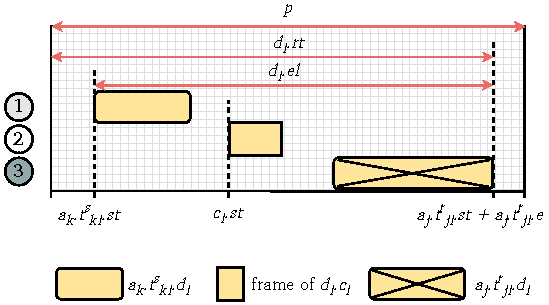
\includegraphics[width=0.75\textwidth]{figures/latency.pdf}
    	\caption{ End-to-end latency and response time for a communication message~($d_i.el$ and $d_i.rt$, respectively). Number one indicates $a_k.t_{ik}^{s}$ slot, as a sender, number two represents $c_i$ frame. As a receiver, $a_j.t_{ji}^{r}$ slot is shown by number three~\cite{askaripoor2023designer}.}
    	\label{fig4_new}
        \end{figure}
    
    As an example, ADAS relies on real-time communication between sensors and other systems; high latency can lead to delays in processing critical information and may negatively impact the performance of the system.
    Another example can be a car equipped with a sensor that detects obstacles in the road. If the sensor sends a message to the car's HPCU indicating that an obstacle is present, the HPCU needs to process this information and take the appropriate action (such as applying the brakes) as quickly as possible. If the end-to-end latency is too high, there may be a delay between when the obstacle is detected and when the car takes action, which can result in a dangerous situation.
    To reduce the end-to-end latency in automotive communication, various measures can be taken, such as optimizing the communication protocol, using high-speed communication technologies, and minimizing the processing time required by the devices during the design phase.
    %%%%%%%%%%%%%%%%%%%%%%%%%%%%%%%%%%%%another explaination-----------------------------
    %End-to-end latency is influenced by several factors, including the speed of the communication network, the distance between the devices, and the processing time required by the devices. In the automotive real-time communication domain, it is important to minimize end-to-end latency as much as possible to ensure safe and reliable operation of the car.
     
    Based on Figure~\ref{fig4_new}, the end-to-end latency of a communication message ($d_i.el$) is the time between the start of the application thread acting as the sender ($a_k.t_{ki}^{s}.st$) and the finishing of the application thread operating as the receiver ($a_j.t_{ji}^{r}.st + a_j.t_{ji}^{r}.e$) of its message chain ($d_i.ch_i$) (see Eq.~(\ref{eq16}) and Figure~\ref{fig4_new})~\cite{askaripoor2023designer}.
    
    %Based on figure~\ref{fig4_new}, the end-to-end latency of a communication message ($d_i$) is the time between the start of the first thread as the sender ($t_i^{s}.st$) and the finishing of the last thread as the receiver ($t_i^{r}.st + t_i^{r}.e$) of its message chain ($d_i.ch_i$) (See equation~(\ref{eq16})).\newline
    
    \begin{equation}
    	%\boldmath
    	d_i.el = a_j.t_i^{r}.st + a_j.t_i^{r}.e - a_i.t_i^{s}.st.
    	\label{eq16}
    	%   \unboldmath
    \end{equation}\newline 
    
    %figure~\ref{fig4_new} depicts an example of end-to-end latency computation for a communication message which its message chain comprises two threads belonging to two various applications and a communication task. To minimize the end-to-end latency of each communication message (\ref{eq17}) is applied.\newline

    Figure~\ref{fig4_new} depicts an example of an end-to-end latency computation for a communication message where the message chain comprises two threads belonging to various applications and a communication task. To minimize the end-to-end latency of each communication message, (\ref{eq17e}) is applied as an optimization goal. In addition, a hard constraint, as~(\ref{eq200}), can be used to limit the end-to-end latency to under a specific maximum bearable value, interpreted as a boundary condition.\newline

    $\forall i \in \mathbb{N}; d_i \in\mathcal{D}$:
    \begin{equation}
    	%\boldmath
    	%\textnormal{Minimize}    
    	el^{i}_{min} = min ({d_i.el})  
    	\label{eq17e}
    	%   \unboldmath
    \end{equation}
    
    \begin{equation}
	%\boldmath
	%\textnormal{Minimize}    
	d_i.el \leq d_i.el_{max}.
	\label{eq200}
	%   \unboldmath
    \end{equation}
 
    %In addition, a hard constraint can be applied to limit the end-to-end latency to under a specific value as a maximum bearable end-to-end latency.

    \subsection{Response Time}
    
    Response time refers to the time it takes for a system to respond to a request or input. This metric is important because it reflects the system's ability to process requests quickly and efficiently. A low response time means that the system is able to handle requests quickly and respond promptly~\cite{zhang2014task}. In the automotive real-time communication domain, response time is critical because it affects the safety and efficiency of the vehicle. For example, if a vehicle's communication system takes too long to respond to a request from the driver or another system, it can cause a delay or malfunction that can lead to an accident. For example, if a car's brake system has a slow response time, it may take longer for the brakes to engage, potentially leading to an accident. Similarly, suppose car's navigation system has a slow response time. In that case, it may take longer to update and provide accurate directions, leading to delays and potential confusion for the driver. Therefore, the communication system needs to have a fast response time in order to ensure the safety and smooth operation of the vehicle.
    %%%%%%%%%%%%%%%%%%%%%%%%%%%%%%%%%%%%%%%%%%%%%%%%%%%%%%%%%%%%%%%%%%%%%%%%%%%%%%%%%%%%%%%%%%
    %Response time refers to the amount of time it takes for a system or device to respond to a request or input. In the automotive real-time communication domain, response time is critical because it affects the safety and efficiency of the vehicle.  It is important for automotive systems to have a quick response time in order to ensure the smooth operation and safety of the vehicle.
    
    The presented computer-aided tool supports the response time optimization as well as the response time condition for a communication message.
    The response time of a communication message ($d_i.rt$) is explained as the time between the beginning of a period, represented as $p.st$, and the time when the job of the last thread in the corresponding message chain is finished~\cite{askaripoor2023designer}. It is given by\newline
    %The response time of a communication message is explained as the time when the job of the last thread in the corresponding message chain is finished from the beginning of a period and it is given by~(\ref{eq18}).
    \begin{equation}
    	%\boldmath
        d_i.rt = a_j.t_{ji}^{r}.st + a_j.t_{ji}^{r}.e - p.st.
    	\label{eq18}
    	%   \unboldmath
    \end{equation}\newline
    
    Figure~\ref{fig4_new} shows an example of the response time for a communication message ($d_i$) similar to the end-to-end latency. 
    In practice, because of the unavailability of resources, $a_k.t_{ki}^{s}.st \neq $~$p.st$. Note that if $a_k.t_{ki}^{s}.st = p.st$, the response time becomes equal to the end-to-end latency ($d_i.el = d_i.rt$). Like the end-to-end latency optimization objective, to minimize the response time, which is stated as a time limit that the information of time-triggered systems requires to be updated within this time bound, the Eq. (\ref{eq19}) is presented. Similar to the end-to-end latency, condition (\ref{eq20}) can be specified as a boundary constraint to enforce the response time to be within a tolerable maximum limit.\newline
    
    
    %figure~\ref{fig4} shows an example of response time for a communication message $d_i$ similar to the end-to-end latency. Probably, because of the unavailability of resources, $a_i.t_i^{s}.st \neq $ \textit{starting of the period}~($p$). Note that if $a_i.t_i^{s}.st = $ \textit{starting of the period}, the response time becomes equal to the end-to-end latency ($d_i.el = d_i.rt$). Like the end-to-end latency, to minimize the response time, which is stated as a time limit that the information of time-triggered systems requires to be updated within this time bound, the equation (\ref{eq19}) is presented.\newline
    
    
    $\forall i \in \mathbb{N}; d_i \in\mathcal{D}$:
    \begin{equation}
    	%\boldmath
    	%\textnormal{Minimize}    
         rt^{i}_{min} = min ({d_i.rt})  
    	\label{eq19}
    	%   \unboldmath
    \end{equation}

    \begin{equation}
    	%\boldmath
    	%\textnormal{Minimize}    
    	d_i.rt \leq d_i.rt_{max}.
    	\label{eq20}
    	%   \unboldmath
    \end{equation}\newline
    %Similar to end-to-end latency, the condition (\ref{eq20}) can be specified to enforce the response time to be on a maximum tolerable bound.\newline
    

   \textbf{Hint}: Note that multicast messages are treated as separate messages when calculating the end-to-end latency. Therefore, the end-to-end latency for a multicast message is determined by the maximum of the individually calculated latencies. Furthermore, each route has its latency for redundant and homogeneous redundant routes, and the maximum latency is considered the final latency for a redundant message. The same policy is applied to the response time.
    
    %\textbf{End-To-End Latency}:
    
    
    
    %\textbf{Response Time}:
    
    
    \subsection{Resource Utilization (RU)}
    
    Resource usage optimization is crucial for embedded system developers to avoid facing limited resources. Load balancing can prevent irregularly overloading some control nodes while leaving others idle. Therefore, a boundary condition and an optimization goal are defined to automatically assign applications to available resources, such as ECUs and HPCUs, including cores and processors, while satisfying the resource usage rule. 

    Based on Eq.~\eqref{eqr21}, as an optimization goal, the number of mapped applications on each control node is minimized, i.e., the applications $a_j$ are distributed on control nodes $n_i^{cz}.a_j$ possibly to keep load balancing of each control node the same~\cite{askaripoor2023designer}. %Furthermore, similar to the last two optimization goals, a hard constraint can be formulated to restrict the number of assigned applications on each control node to a maximum mapped number as following.\newline 
    The Eq.~\eqref{eqr22} is utilized to average the usage of control nodes as a boundary constraint. The number of mapped applications on each control node must be greater than or equal to a tolerable bound denoted as the $apn$ value, which is the total number of applications divided by the total number of control nodes according to Eq.~\eqref{eqr22}. As a result, the applications are as equally as possible distributed on control nodes to maintain the load balancing of each control node. Condition \eqref{eqr022} shows a boundary constraint similar to Eq. \eqref{eqr22}, which is considered for control node cores such as HPCU cores and $apc$, indicating a bearable limit~\cite{askaripoor2023designer}.\newline
    
     %\newline
    
    $\forall i,j \in \mathbb{N}; m_{ij} \in\mathcal{M}; a_j \in\mathcal{A}; {n_{i}^{cz}} \in \mathcal{N}$: 
     
    \begin{equation}
    	%\boldmath
    	%\sum_{m_s=(A_{sen}, N_s) \in m, m\in M } m_{s}=1	
    	%i, j \in \mathbb{N} 
    	ru^{i}_{min} = min (\sum_{j \in \mathbb{N}} {m_{ij}}.{n_i^{cz}}.a_j) 
    	\label{eqr21}
    	%   \unboldmath
    \end{equation}
    
    
    \begin{equation}
    	%\boldmath
    	%\textnormal{Minimize}    
    	\sum_{j \in \mathbb{N}} {m_{ij}}.{n_i^{cz}}.a_j \geq apn
    	\label{eqr22}
    	%   \unboldmath
    \end{equation}

    \begin{equation}
    	%\boldmath
    	%\textnormal{Minimize}    
    	\sum_{j \in \mathbb{N}} {m^{c}_{ij}}.{n_i^{cz_c}}.a_j \geq apc.
    	\label{eqr022}
    	%   \unboldmath
    \end{equation}
    
    \subsubsection{Maximum Resource Usage}
    It is necessary to consider maximum resource utilization, such as the maximum usage of memory and processor of an ECU, due to vehicle software updates. In other words, a specific amount of memory and processor usage must be left intact during the design-time configuration process, as a vehicle software update may require extra memory and processor capacities.
     The updated software may put additional load on the processor; therefore, ensuring that the processor can handle the increased computational requirements without affecting the overall system performance is required. This can be achieved by having enough unused processor usage and sufficient computational power on the processor~\cite{askaripoor2022architecture, askaripoor2023designer}.\newline 
    
    %
    
    \textbf{Memory}:
        The amount of available memory on the ECU should be determined, and the memory requirements of the updated software should be assessed. It must be ensured that the new software fits the memory constraints and leaves enough space for other critical functions. Hence, the proposed tool considers the maximum memory utilization, formulated as Eq.~(\ref{eq022}). Based on this boundary condition, the sum of application memories that is mapped on $n_i^{cz}$ must be within the maximum memory capacity of the node ($n_i^{cz}.m_{max}$)~\cite{askaripoor2023designer}.\newline
  

    $\forall i,j \in \mathbb{N}; m_{ij} \in\mathcal{M}; a_j \in\mathcal{A}; {n_{i}^{cz}} \in \mathcal{N}$: 
    
    \begin{equation}
    	%\boldmath
    	%\textnormal{Minimize}    
    	\sum_{j \in \mathbb{N}} ({m_{ij}}.{n_i^{cz}}.a_j\times a_j.mu) \leq {n_i^{cz}}.m_{max}.
    	\label{eq022}
    	%   \unboldmath
    \end{equation}\newline

      \textbf{ECU}:
    Resource usage optimization is important to embedded systems developers to avoid facing limited resources. Moreover, the load balancing scenario, which is the process of distributing a set of tasks over a set of resources, plays a pivotal role in overall processing and makes it more efficient. Using load balancing avoids irregularly overloading some control nodes while others are idle. Therefore, to automatically assign applications to available resources, e.g., ECU, HPCU including core and processor while optimizing the resource usage, an optimization goal is defined and integrated into presented the model-based framework using Eq.~(\ref{eq21}) to minimize the control nodes utilization~\cite{askaripoor2023designer}.\newline
    
    
    
    $\forall i,j, m_i \in\mathcal{M},  a_j \in\mathcal{A}, {n_{i}^{cz}} \in \mathcal{N}$:
    \begin{equation}
    	%\boldmath
    	%\sum_{m_s=(A_{sen}, N_s) \in m, m\in M } m_{s}=1	
    	%i, j \in \mathbb{N} 
    	ru_{min} = min (\sum_{j \in \mathbb{N}} {m_j}.{n_i^{cz}}.a_j) 
    	\label{eq21}
    	%   \unboldmath
    \end{equation}
    , based on Eq.~(\ref{eq21}), the number of mapped applications on each control node is minimized, i.e., the applications $a_j$ are equally distributed on control nodes $n_i^{cz}.a_j$ possibly to keep load balancing of each control node the same. Furthermore, similar to the last two optimization goals, a hard constraint can be formulated to restrict the number of assigned applications on each control node to a maximum mapped number as follows.\newline      
      
      
      
    $\forall i, n_i^{cz} \in\mathcal{N} $:
    \begin{equation}
    	%\boldmath
    	%\textnormal{Minimize}    
    	n_i^{cz}.ru \leq n_i^{cz}.ru_{max}. 
    	\label{eq22}
    	%   \unboldmath
    \end{equation}
    
    %\subsection{Maximum Resource Usage}
    %\subsubsection{Memory Usage}
    %\subsubsection{ECU Usage}
    
  
    
    
    
    \subsection{Load Balancing in Vehicle Communication Network} 
    
    Overloading of communication links in automotive networks can occur when the network experiences a higher volume of data traffic than it can handle. As vehicles become more connected and advanced, the demand for data transmission between various components and systems increases, which can strain the communication infrastructure. This overload can lead to delays in message delivery, increased latency, and even system failures.
    Load balancing is also a technique used to manage communication messages in a network.
    It aims to evenly distribute the communication traffic across these links, avoiding overutilizing any specific path and maximizing the network's capacity. This helps prevent bottlenecks, reduces latency, and improves overall network performance.
    %In automotive networks, multiple communication links or routes may exist between different components or systems within the vehicle. Load balancing aims to evenly distribute the communication traffic across these links, avoiding overutilization of any specific path and maximizing the network's capacity. This helps prevent bottlenecks, reduces latency, and improves overall network performance.
    Communication messages or data packets can be distributed across multiple links based on predefined load-balancing algorithms. %These algorithms consider factors like current link utilization, available bandwidth, and link characteristics to determine the optimal distribution strategy. 
    
    %Common load balancing algorithms include round-robin, weighted round-robin, least-connections, or adaptive load balancing based on real-time metrics.
    \subsubsection{Link Occupation Rate (LOR)}
    
    The presented tool helps to reduce the overall density of communication tasks and prevents the overloading of links. It also decreases the number of scheduling competitions which mitigates the system's complexity, resulting in shorter synthesis times. To accomplish this, the introduced framework uses an optimization objective as \eqref{eql23} that assists in lessening the LOR ratio~\cite{askaripoor2023designer}.\newline
    %According to \eqref{eql23}, during exploration of message routing for each communication message $d_i$, the sum of possible outgoing messages $d_i^{out}$ over each link $l_j$ must be minimized, leading to frame balancing for each link. Correspondingly to the last optimization goals, the LOR can also be forced to be within a maximum acceptable bound by specifying a boundary constraint as \eqref{eql24}.\newline
    
    
        
    %Similar to the control nodes, load balancing for communication messages routed over the links is applied to reduce the total density of the competing communication tasks over each link and to avoid overloading of the communication links. In addition, the fewer scheduling competitions of the frames the less complexity of the constraint system which needs to be solved and leads to less synthesis time. To reduce the LOR, we define the following equation:\newline
    
    
    
    
   $\forall i,j \in \mathbb{N}; d_i^{out} \in\mathcal{D}; l_j \in\mathcal{L}$:
    \begin{equation}
    	%\boldmath
    	%\textnormal{Minimize}    
    	  lor_{min} =  min (\sum_{i \in \mathbb{N}} d_i^{out}.l_{j})  
    	\label{eql23}
    	%   \unboldmath
    \end{equation}
    
    \begin{equation}
    	%\boldmath
    	%\textnormal{Minimize}    
    	 \sum_{i \in \mathbb{N}} d_i^{out}.l_{j} \leq l_j.lor_{max}  
    	\label{eql24}
    	%   \unboldmath
    \end{equation}\newline
   , according to Eq. \eqref{eql23}, during exploration of message routing for each communication message $d_i$, the sum of possible outgoing messages $d_i^{out}$ over each link $l_j$ must be minimized, leading to frame balancing for each link. Correspondingly to the last optimization goals, the LOR can also be forced to be within a maximum acceptable bound by specifying a boundary constraint as \eqref{eql24}~\cite{askaripoor2023designer}.
    
    %Based on (\ref{eql23}), during exploration of message routing for each communication message $d_i$, the sum of possible outgoing messages $d_i^{out}$ over each link $l_j$ must be minimized resulting in frame balancing for each link. Correspondingly to the last optimization goals, the LOR can also be forced to be within a maximum tolerable bound by specifying a hard constraint as (\ref{eql24}).\newline
    

    
    
    \subsubsection{Maximum Bandwidth Utilization}
    
    By defining the maximum bandwidth usage for each communication link, E/E system integrators can efficiently allocate the available network resources. It allows them to ensure that critical systems and applications receive the necessary bandwidth to function reliably. It helps prevent network overloading and ensures bandwidth is distributed appropriately among different components.
    E/E architects can optimize the overall network's performance by setting maximum bandwidth limits, and they can analyze the bandwidth requirements of different components and applications and design the network topology accordingly. This allows them to avoid bottlenecks and ensure smooth data flow within the network. In some cases, automotive networks may need to provide guarantees on bandwidth availability. For instance, certain data transmissions must occur within specific time constraints in time-critical applications like autonomous driving. Specifying maximum bandwidth utilization ensures that the required bandwidth is reserved and available when required.
    For future scalability and expansion of the network, considering maximum bandwidth utilization helps. As automotive technologies evolve and new applications are introduced, the bandwidth requirements may change. By defining the maximum bandwidth usage in the design phase, future growth can be accommodated and ensured that the network can handle increased data volumes and communication demands~\cite{askaripoor2023designer}.
    
    Therefore, the LOR constraint can be extended by adding the bandwidth of each link to ensure that each network link's maximum bandwidth utilization is not exceeded during finding message paths. This leads to condition (\ref{eq023}), which states that the sum of bandwidths used by communication tasks over each link $l_j$ must be less than or equal to the maximum bandwidth specified by the user for the same link ($l_{j}.bw_{max}$). Here, $transT$ represents the transmission time of each frame~\cite{askaripoor2023designer}.\newline
    
    $\forall i,j \in \mathbb{N}; d_i^{out} \in\mathcal{D}; l_j \in\mathcal{L}$:
        \begin{equation}
    	\small
    	%\boldmath
    	%\textnormal{Minimize}    
    	     \sum_{i \in \mathbb{N}} (d_i^{out}.l_{j} \times  d_i^{out}.c_{i}.fl/transT) \leq l_{j}.bw_{max}.
    	\label{eq023}
    	%   \unboldmath
    \end{equation}
    
    
    \subsection{Cost Reduction (CR)} 
    
    Cost optimization in automotive network topologies involves designing and implementing network architectures that balance cost efficiency and performance.
    Since each communication link in the E/E Designer can have different types, such as Ethernet, FlexRay, and TTCAN-bus, and subsequently varying costs, a cost optimization goal constraint is defined \eqref{eq25} to minimize the cost of the created paths. Similarly, this objective can be applied to other software/hardware components~\cite{9565115, 9613692, 9212001,askaripoor2023designer}.\newline
    
    %To optimize the cost of created routes since each communication link in the \textit{E/E Designer} can have different types e.g., Ethernet, FlexRay, and CAN-bus, and subsequently various costs, we also define the cost optimization objective~(\ref{eq25}) to minimize the cost of created paths regarding the user demand. Similarly, this can be applied to the other SW/HW components.\newline
    
    
    $\forall i,j, d_j^{out} \in\mathcal{D}, l_i \in\mathcal{L}$:
        \begin{equation}
        	%\boldmath
        	%\textnormal{Minimize}    
        	cr_{min} =  min (\sum_{i \in \mathbb{N}} cost.d_j^{out}.l_{i})  
        	\label{eq25}
        	%   \unboldmath
        \end{equation}
    
        \begin{equation}
    	%\boldmath
    	%\textnormal{Minimize}    
    	\sum_{i \in \mathbb{N}} cost.d_j^{out}.l_{i} \leq path.cost_{max}.
    	\label{eq026}
    	%   \unboldmath
        \end{equation}\newline
    
    In Eq.~\eqref{eq026}, the cost of a chosen path is forced to be less than or equal to the boundary cost value of a path specified by the user. This is considered a cost boundary constraint~\cite{askaripoor2023designer, 9565115}.
    
    %In equation~(\ref{eq25}), the cost of a selected route including link/links must be less than or equal to the specified cost of a path defined by the user. This is considered as a cost boundary constraint. 
    
    \subsection{Reliability}
    
    
    Reliability is an essential concept in the context of ISO 26262~\cite{iso26262} because it is one of the critical factors that must be considered when designing and implementing safety-related systems. Reliability refers to the ability of a system or component to perform its intended function consistently and without failure over a specified time, as expressed in Chapter~\ref{basicConcepts}.
    There are several ways in which reliability is addressed in ISO 26262~\cite{iso26262}, including reliability models and reliability testing. Reliability models are mathematical models that are used to predict the probability of failure of a system or component based on various factors, such as operating conditions and environmental factors. Reliability testing involves subjecting a system or component to simulated or actual operating conditions in order to measure its performance and identify any potential failure points~\cite{xie2018reliability}.
    
    In addition to reliability models and testing, ISO 26262 also specifies requirements for the design and implementation of safety measures, such as redundant systems and fail-safe mechanisms, to ensure the reliability of safety-related systems. To compute the reliability, there are various metrics which can be used. For instance, the failure rate of E/E system components can be defined by E/E architects, and the reliability, e.g., routing and mapping, can be calculated accordingly.
    As stated in Chapter~\ref{basicConcepts}, our proposed tool follows the component-based approach using the reliability RBD method~\cite{international2017electric, Menčík16}.
          \begin{figure}[t]
    	\centering
    	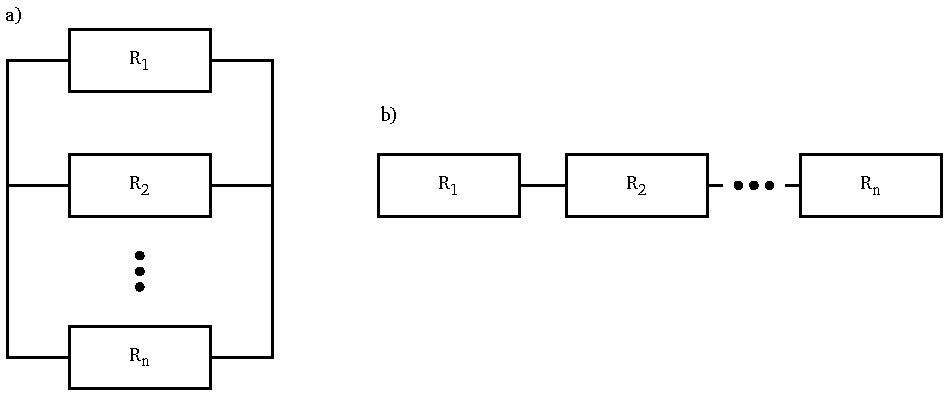
\includegraphics[width=1\textwidth]{figures/reliability.pdf}
    	\caption{ a) A parallel system including multiple elements. b) A series system comprising multiple elements.}
    	\label{fig4_reli}
    \end{figure}
    
    %The details of metrics and the reliability formulation are explained in the following~\cite{askaripoor2022architecture}.
    
    %The integration of reliability into E/E Designer follows a component-based approach inspired by the reliability block diagram (RBD) method in a sense that the overall reliability prediction is calculated by looking at the individual components of the system while considering serial and parallel component configurations as depicted in 
    According to Figure~\ref{fig4_reli}, the reliability can be computed by considering individual components of the system and taking serial and parallel configurations into account~\cite{Menčík16}. 
    Firstly, the user specifies the reliability/failure rate for each individual (hardware) component. These failure rates can be obtained from norms, data sheets, field experience values, or by exploring thermal, electrical, or mechanical mission profiles.
    Secondly, the overall reliability score of the system is calculated from the individual reliability scores; thirdly, the computed overall reliability score is constrained by an expected reliability score. Alternatively, constraints can be formulated by requiring reliability scores for sub-systems. These expected reliability scores can be derived from required ASIL levels.

     In a series system, as depicted in Figure~\ref{fig4_reli} (b), the failure of any component can lead to the failure of the entire system. Therefore, the overall reliability of the series system can be calculated as the product of the individual reliabilities~\cite{Menčík16}:
    
    \begin{equation}
    R_s(t) = \prod_{i=1}^n R_i(t).
    \label{reli_main}
    \end{equation}
    

    Given that $\lambda_i$ represents the failure rate and $R_i$ indicates the reliability of the i-th component:
    
    \begin{equation}
        R_i(t) = e^{-\lambda_i t}
        \label{eq:individual_reliability}
    \end{equation}
    and considering Eq. \eqref{reli_main}, Eq. \eqref{eq:individual_reliability} can be expressed as follows:
        
    \begin{equation}
            R_s(t) = e^{-(\sum_{i=1}^n \lambda_i) t}.
    \end{equation}

    
    
    
    A parallel system, as shown in Figure~\ref{fig4_reli}~(a) and which models redundancy, only fails if all its components fail. As a result, the system reliability is calculated as follows~\cite{Menčík16}:
    \begin{equation}
        R_p(t) = 1 - \prod_{i=1}^n (1 - R_i(t))
        \label{rp_1}
    \end{equation}
    and by using the Eq. \eqref{eq:individual_reliability}, Eq.~\eqref{rp_1} can be stated as below
    
    \begin{equation}
         R_p(t) = 1 - \prod_{i=1}^n (1 - e^{\lambda_i t}) = \sum_{i=1}^n e^{-\lambda_i t} - e^{-(\sum_{i=1}^n\lambda_i) t}.
    \end{equation}
    

    
    
    
    \subsubsection{MTTF}
    
    As mentioned in Chapter~\ref{basicConcepts}, MTTF stands for mean time to failure, and it is a commonly used metric in the automotive domain and other engineering fields. MTTF represents the average time elapsed between the start of a system or component's operation and the occurrence of its first failure. It is a measure of reliability and indicates the expected lifespan of a component or system under normal operating conditions.
    In the automotive domain, MTTF assesses the reliability of various vehicle components such as engines, transmissions, electrical systems, braking systems, and other critical parts.
    Depending on the specific application, MTTF is typically expressed in time units, such as hours, miles, or kilometers. It is an important factor considered during automotive systems' design and development stages to ensure that they meet the required reliability standards and customer expectations~\cite{askaripoor2023designer,askaripoor2022architecture}.
    
     As stated in Chapter~\ref{basicConcepts}, if the failure rate remains constant over time, it can be assumed that
    
    \begin{equation}
    MTTF = \frac{1}{\lambda}
    \label{mttf_4}
    \end{equation}
    , and taking Eq.~\eqref{mttf_4} into account, the MTTFs for the series and parallel systems, as visualized in Figure~\ref{fig4_reli}, are computed using Eqs. \eqref{eq:mttf_seq} and \eqref{mttf_para}, respectively, as follows~\cite{Menčík16}: 
    

    \begin{equation}
        MTTF_{seri} = \int_0^{\infty} e^{-(\sum_{i=1}^n \lambda_i) t} dt = \frac{1}{\sum_{i=1}^n \lambda_i}
        \label{eq:mttf_seq}
    \end{equation}
    \vspace{5pt}
            
    \begin{equation}
         MTTF_{par} = \int_0^{\infty} \sum_{i=1}^n e^{-\lambda_i t} - e^{-(\sum_{i=1}^n \lambda_i) t} dt
         = \sum_{i=1}^n \frac{1}{\lambda_i} - \frac{1}{\sum_{i=1}^n \lambda_i}.
         \label{mttf_para}
     \end{equation}
    \vspace{3pt}
    
     To calculate the reliability of a path in an automotive network when the failure rate or MTTF of each link is provided as a constant value, a similar approach to the one used for the series and parallel systems can be applied.
     
    \subsubsection{Single Message Routing}
        
        %The introduced framework, calculate the reliability of the entire path by multiplying the reliabilities of all activated links since they are in series and the calculation is performed in a single-step. Since the reliability is specified as a boundary constraint as well as an optimization objective in the E/E Designer, during the process of creating paths for communication messages from senders to receivers, the reliability of each possible path is computed and therefore the generated route meets the reliability boundary value (See equations \eqref{reli_sing} and \eqref{reli_sing1}). The same method is used for finding the most optimized route in terms of reliability.
        
        The introduced framework calculates the reliability of the entire path by multiplying the reliabilities of all activated links, as they are in series, and this calculation is performed in a single step. Reliability is specified as a boundary constraint and an optimization objective in the proposed tool. During the process of creating paths for communication messages from senders to receivers, the reliability of each possible path is computed, ensuring that the generated route meets the specified reliability boundary value (see Eqs. \eqref{reli_sing} and \eqref{reli_sing1}). The same method is employed to find the most optimized route regarding reliability~\cite{10588416}.
        
    
    \begin{equation}
        R_{single}(t) = \prod_{i=1}^n R_{l_i}(t)
    \label{reli_sing}
    \end{equation}
    
    \begin{equation}
        R_{single}(t) = e^{-(\sum_{i=1}^n d^{i}_{out}.l_i.\lambda_i) t}
            \label{reli_sing1}
    \end{equation}
    
        
    \begin{equation}
           MTTF_{single} = \int_0^{\infty} e^{-(\sum_{i=1}^n d^{i}_{out}.l_i.\lambda_i) t} dt = \frac{1}{\sum_{i=1}^n d^{i}_{out}.l_i.\lambda_i}.
               \label{mttf_sing}
    \end{equation}
    %Based on \eqref{reli_sing1}, reliability of each single path is only calculated for activated links. This decision of which links are activated, depends on the failure rate of each link as the reliability goals intended to be optimized. The MTTF for a single path is computed based on \eqref{mttf_sing} where only the failure rates for activated links are considered.  
    
    Based on Eq. \eqref{reli_sing1}, the reliability of each path is calculated only for the activated links. Determining which links are activated depends on the failure rate of each link, as it aligns with the intended reliability optimization goals. In addition, the MTTF for a single path is computed according to Eq. \eqref{mttf_sing}, where only the activated links' failure rates are considered.
    
    
    
    \subsubsection{Redundant Message Routing}
    The reliability formula for the parallel system, as explained in Eq. \eqref{rp_1}, is employed to calculate the reliability for redundant paths. According to \eqref{reli_redun}, the reliability for the redundant message routing, which consists of two single paths (depicted as the upper limit of the product in Eq. \eqref{reli_redun}, is computed by treating each single path, as part of the redundant routings, as an element of a parallel system containing two elements. In Eq. \eqref{reli_redun}, the single path's reliability is obtained similar to Eq. \eqref{reli_sing}~\cite{10588416}.
    
    \begin{equation}
     R_{redundant}(t) = 1 - \prod_{j=1}^2 (1 - R_{single_j}(t)).
     \label{reli_redun}
    \end{equation}
    
    %Note that in our proposed system model, the uncertainty of the reliability is not considered. In other words, the failure rates of the E/E components, given by the user, are constant values and not intervals. This means that the uncertain optimization is not included in the above constraints.
    In the proposed system model, the uncertainty of reliability is not taken into account. This means that the failure rates of the E/E components, as provided by the user, are treated as fixed values, not as ranges. In other words, uncertain optimization is not included in the above-mentioned equations.
    
    %\subsubsection{Mapping} 
    
    
    
    %In this example, the bottom-most interface device is shared among both partitions. The sharing of the interface is realized by introducing virtual links that connect the partitions with the interface. Thus, messages can be transported between the interface and App 2 or App 3 in parallel, however, only one communication message can be transported between the ECU and the interface at a time. Thereby, only the interface device, which is subject to the hypervisor, controls the flow of messages.
        \begin{figure}[ht]
    	\centering
    	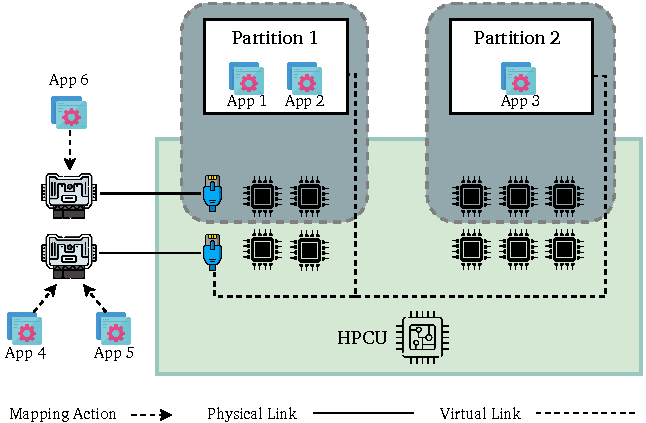
\includegraphics[width=0.9\textwidth]{figures/hypervisor_req.pdf}
    	\caption{ Graphical representation of the functioning of the hypervisor constraints implemented in the meta-model presented in Chapter~\ref{method}, exemplified by the transmission of communication messages. This exemplary scenario shows an HPCU comprising 10 CPU cores and two communication interface devices running two partitions. Partition 1 has exclusive control over two cores and one interface device, while partition 2 controls three cores, as indicated by the dark green boxes. The rest of the CPU cores and the other interface device are shared among both partitions. Assume that communication messages are sent between a$_1$ and a$_6$, a$_2$ and a$_4$, and a$_3$ and a$_5$. The two concepts of exclusive resource allocation and resource sharing are shown in this figure~\cite{10588416}.}
    	\label{fig_hyp}
        \end{figure}
    \subsection{Hypervisor-related Constraints}
        
        Virtualization is increasingly important in the automotive industry as it can facilitate many aspects of the E/E design process by improving flexibility, efficiency, and security. This technology is explained in Chapter~\ref{basicConcepts}. This section explains the hypervisor-related constraints integrated into the E/E Designer tool~\cite{10588416}.  
            
        \subsubsection{Exclusive Resource Allocation for Partitions of Type-1 Hypervisor}    
        %A fundamental aspect of hypervisor technologies is the exclusive allocation of resources which refers to the practice of dedicating specific hardware resources to individual virtual machines. This ensures that each VM has its own isolated portion of CPU, memory, storage, and other hardware resources, preventing interference and contention among VMs.In safety-critical systems like for automotive applications, sharing of critical resources like the CPU is generally not a common practice because of their stringent requirements for reliability, predictability, and fault tolerance. Sharing CPU resources among multiple tasks or applications introduces uncertainty and potential contention for processing time, which can lead to unpredictable behavior and jeopardize the safety of the system.            In the \textit{E/E Designer}, the exclusive resource allocation is realized by treating each component of the virtualized hardware as an independent component. Thereby, the exclusivity of these resources is captured by the mapping and routing constraints already defined in the framework. As an example, figure~\ref{fig_hyp} shows a hardware platform running a hypervisor which includes two partitions. As the exclusive resource allocation, since in the modeling, partition 1 and all its exclusively used resources are treated as a stand-alone node, the exclusiveness of the communication interface device and the two CPU cores is implicitly fulfilled. The physical link is only available to transport communication messages between App 1 and App 6 without enforcing it via an explicit constraint.
        
        
        A fundamental aspect of hypervisor technologies is the exclusive allocation of resources, which refers to dedicating specific hardware resources to individual virtual machines. This ensures that each VM has its isolated portion of CPU, memory, storage, and other hardware resources, preventing interference and contention among VMs~\cite{9968908}.
        In safety-critical systems, such as those used in automotive applications, sharing critical resources like the CPU is generally not a common practice due to stringent requirements for reliability, predictability, and fault tolerance. Sharing CPU resources among multiple tasks or applications introduces uncertainty and potential contention for processing time, leading to unpredictable behavior and jeopardizing the system's safety.
        In the proposed framework, exclusive resource allocation is realized by treating each component of the virtualized hardware as an independent entity. Thus, the exclusivity of these resources is captured by the mapping and routing constraints already defined in the framework. For example, Figure~\ref{fig_hyp} shows a hardware platform running a hypervisor with two partitions. Through exclusive resource allocation, partition 1 and all its exclusively used resources are treated as stand-alone nodes in the modeling, implicitly ensuring the exclusiveness of the communication interface device and the two CPU cores. The physical link is only available to transfer communication messages between a$_1$ and a$_6$ without requiring an explicit constraint~\cite{10588416}.
        
            
        %In the E/E Designer for modeling the the type-1 hypervisor, an interface to the environment is developed. Based on this interface, only one partition at a time can access to the HPCU resources such as processor, RAM, Memory, ports, etc. 
        
    
        
        %consider different virtualized CPU cores that are each used by fully isolated VMs. Assuming there is no inter-VM communication, all cores can be considered to run independently and in parallel.


            \begin{figure}[b!]
    	\centering
    	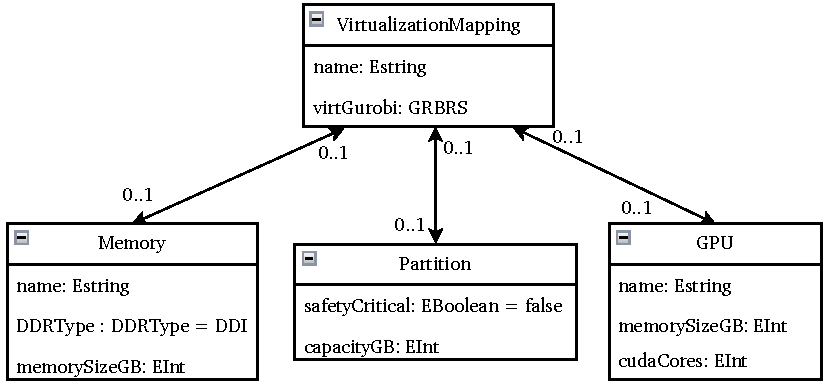
\includegraphics[width=1\textwidth]{figures/metamodel_hypervisor.pdf}
    	\caption{ The UML classes required for the hypervisor-related constraints.}
    	\label{fig_uml}
        \end{figure}







        \begin{comment}
        \begin{figure*}
        \centering
        \begin{tikzpicture}
        %\tikzset{dark box/.style={draw,fill=gray!80,rounded corners, minimum height=0.5cm, minimum width=2cm}}   
        \begin{class}{VirtualizationMapping}{0,0}
        \small
        \attribute{name : EString}
        \attribute{virtGurobi : GRBRS}
        \end{class}
        
        \begin{class}{Partition}{0,-4}
        \small
        \attribute{safetyCritical : EBoolean = false}
        \attribute{capacityGB : EInt}
        \end{class}
        
        \begin{class}{GPU}{6,-4}
        \small
        \attribute{name : EString}
        \attribute{memorySizeGB : EInt}
        \attribute{cudaCores : EInt}
        \end{class}
        
        \begin{class}{Memory}{-6,-4}
        \footnotesize
        \attribute{name : EString}
        \attribute{DDRType : DDRType = DDI}
        \attribute{memorySizeGB : EInt}
        \end{class}
        
        \unidirectionalAssociation{VirtualizationMapping}{0..1}{}{Partition}
        \unidirectionalAssociation{Partition}{}{0..1}{VirtualizationMapping}
        \unidirectionalAssociation{VirtualizationMapping}{0..1}{}{Memory}
        \unidirectionalAssociation{Memory}{}{0..1}{VirtualizationMapping}
        \unidirectionalAssociation{VirtualizationMapping}{0..1}{}{GPU}
        \unidirectionalAssociation{GPU}{}{0..1}{VirtualizationMapping}
        \end{tikzpicture}
        \caption{The UML classes required for the hypervisor-related constraints.}
        \label{fig_uml}
        \end{figure*}
        \end{comment}

        \subsubsection{Resource Sharing Among Partitions of Type-2 Hypervisor}
        %In addition to splitting up the available resources each as a whole, the hypervisor technologies also allow to share certain resources among multiple partitions, as explained in Chapter~\ref{basicConcepts}. In the context of vehicle E/E architectures, resource sharing is usually used for non-critical I/O devices, such as communication interfaces or sensors with less stringent timing requirements, and networking interfaces for diagnostics or non-real-time data transfer.
          
        In addition to splitting up the available resources as a whole, hypervisor technologies also allow the sharing certain resources among multiple partitions, as explained in Chapter~\ref{basicConcepts}. In vehicle E/E architectures, resource sharing is typically used for non-critical I/O devices, such as communication interfaces or sensors with less stringent timing requirements, and networking interfaces for diagnostics or non-real-time data transfer.  
          
           
        %In the \textit{E/E Designer}, this concept is realized through virtual links between the shared interface and the respective partitions. In that way, the shared interface acts as a multiplexer on the partition's messages, imitating the actual physical implementation.
         %In the \textit{E/E Designer}, this concept is realized by introducing virtual links between the shared resource and the respective partitions. Those virtual links are not visible in the front-end but have exactly the same properties as normal links. In the example presented in figure~\ref{fig_hyp}, the bottom-most interface device is shared among both partitions. The sharing of the interface is realized by introducing virtual links that connect the partitions with the interface. Thus, messages can be transported between the interface and a$_2$ or a$_3$ in parallel, however, only one communication message can be transported between the ECU and the interface at a time. Thereby, only the interface device, which is subject to the hypervisor, controls the flow of messages.
         
         In the E/E Designer, this concept is realized by introducing virtual links between the shared resource and the respective partitions. These virtual links are not visible in the frontend but have the same properties as regular links.
        The bottom-most interface device is shared among both partitions in the example presented in Figure~\ref{fig_hyp}. Interface sharing is achieved by introducing virtual links that connect the partitions with the interface. Thus, messages can be transported between the interface and a$_2$ or a$_3$ in parallel; however, only one communication message can be transmitted between the ECU and the interface at a time. Thereby, only the interface device, subject to the hypervisor, controls the flow of messages.
         
         
         
         
         
         %In the UML class diagram shown in figure~\ref{fig_uml}, which is part of the metamodel explained in Chapter~\ref{method}, the VirtualMapping UML class is connected to the hardware resource classes including GPU and memory and the Partition class via bidirectional association relations. Other than that, the VirtualMapping class has the same relationships to other classes than the Link class in order to replicate its functionality. The basic idea is similar to that presented earlier, instead of explicitly programming all the constraints necessary to enforce the correct behavior of all components during resource sharing, the virtual links are a way to encode these constraints into the metamodel. Virtual links mimic the independence of access requests. In that way, the shared interface acts as a multiplexer on the partition's messages, imitating the actual physical implementation.
        
        In the UML class diagram shown in Figure~\ref{fig_uml}, which is part of the metamodel explained in Chapter~\ref{method}, the VirtualizationMapping UML class is connected to the hardware resource classes, including GPU and memory, and the Partition class via bidirectional association relations. Other than that, the VirtualizationMapping class has the same relationships to other classes as the Link class in order to replicate its functionality. The basic idea is similar to that presented earlier. Instead of explicitly programming all the constraints necessary to enforce the correct behavior of all components during resource sharing, the virtual links are a way to encode these constraints into the metamodel. Virtual links mimic the independence of access requests. In that way, the shared interface acts as a multiplexer on the partition's messages, imitating the actual physical implementation~\cite{10588416}.
        
        
        

        
        \subsubsection{Memory Constraint}
        
       Using virtualization, the memory of an HPCU can be shared among multiple partitions. From a modeling perspective, this corresponds to the requirement that the sum of the memory utilization of the individual partitions must be smaller or equal to the total available memory of the HPCU:\newline 
        
        
        $\forall h \in \mathcal{H}:$ \\
        \begin{equation}
        \sum_{i \in \mathbb{N} } p_i.maxMemory \le h.memory.
        \label{memory_con}
        \end{equation}
    
    According to constraint \eqref{memory_con}, the sum of allocated memories for hypervisor partitions running on an HPCU must be less than or equal to the memory capacity of an HPCU. $\mathcal{H}$ indicates a set of HPCUs, and $p$ represents a hypervisor partition executing on an HPCU.
 
    
    \section{Multi-Objective Optimization}
    
    Multi-objective optimization (MOO) is a branch of optimization that deals with problems involving multiple conflicting objectives. In traditional optimization, the goal is to find a single optimal solution that minimizes or maximizes a single objective function. However, in many real-world scenarios, multiple objectives must be simultaneously considered, and these objectives may conflict.
    The MOO aims to find solutions representing the trade-offs between the different objectives rather than a single optimal solution. These solutions are known as Pareto-optimal or non-dominated solutions. A solution is considered Pareto-optimal if no other solution improves one objective without worsening at least one objective~\cite{gunantara2018review, askaripoor2022architecture, 9613692, askaripoor2023designer}.
    
    \subsection{Gurobi Multi-Objective Optimization}
    Gurobi is a widely used commercial optimization solver that provides powerful capabilities for solving optimization problems, including multi-objective optimization. Gurobi supports MOO through its Python interface, allowing users to define and solve problems with multiple goals~\cite{gurobi}. Gurobi solver supports two MOO approaches, each explained below and summarized below.  %Here's an overview of how multi-objective optimization can be performed using Gurobi.
    \subsubsection{Hierarchical Approach}
    
    In a hierarchical or lexicographic approach, a priority is allocated to each objective, and optimization is performed by considering objectives in descending order of priority. At each stage, the best solution for the current objective is determined while ensuring it does not negatively impact the quality of solutions for higher-priority objectives. Priorities for each objective can be specified using the "\textit{setObjectiveN}" function or the "\textit{ObjNPriority}" attribute. Priorities are represented as whole numbers, with higher values indicating higher priorities. The default priority for an objective is $0$.
    For instance, consider a model with two objectives, where the first objective has a priority of $7$ and the second has a priority of $3$. Assuming the optimal solution for the first objective is $80$. In this case, the solver will identify the solution that optimizes the negative of the second objective among all solutions that achieve the first objective value of $100$~\cite{gurobi, askaripoor2023designer}.
    
    %A hierarchical or lexicographic approach assigns a priority to each objective, and optimizes for the objectives in decreasing priority order. At each step, it finds the best solution for the current objective, but only from among those that would not degrade the solution quality for higher-priority objectives. You provide the priority for each objective as an argument to \textit{setObjectiveN}. Alternatively, you can use the \textit{ObjNPriority} attribute. Priorities are integral, not continuous. Larger values indicate higher priorities. The default priority for an objective is 0.
    
    
    
    %To give an example, if your model has two objectives, with priorities $10$ and $5$, and objective weights 1.0 and -1.0. Assuming the optimal solution for the first objective has value $100$, then the solver will find the solution that optimizes minus the second objective from among all solutions with objective $100$ for the first objective.
    
    \subsubsection{Blended Approach}
    
    To generate a single objective, a blending technique combines linearly various objectives by assigning a weight to each objective using the "\textit{setObjectiveN}" function. Alternatively, the default weight of 1.0 can be adjusted by utilizing the "\textit{ObjNWeight}" attribute in conjunction with "\textit{ObjNumber}"~\cite{gurobi}.

    %You should avoid weights that are very large or very small. A very large weight (i.e., larger than $10^6$) may lead to very large objective coefficients, which can cause numerical difficulties. A very small weight (i.e., smaller than $1e-6$) may cause the contribution from that objective to the overall blended objective to be smaller than tolerances, which may lead to that objective being effectively ignored.
    
    \subsection{Multi-Objective Optimization in the E/E Designer Framework}
    
    Given the above representation of the presented tool optimization goals, different classes of objectives can be considered in the MOO problem integrated into the framework. For instance, one combination of objectives can simultaneously minimize the end-to-end latency, response time, LOR, and resource usage, with different predefined priorities as shown in Eq. \eqref{eq026} to \eqref{eq29}. The hierarchical approach, as illustrated above, is utilized where it assigns a priority to each objective and optimizes the objectives in reducing priority order~\cite{askaripoor2023designer}.
    
    
    %The \textit{E/E Designer} embraces the MOO goals to minimize end-to-end latency, response time, resource utilization, and cost reduction simultaneously with different predefined priorities (See (\ref{eq26}) to (\ref{eq29})). 
    
    \begin{equation}
    	%\boldmath
    	%\textnormal{Minimize}    
    	Obj_{1}~(el_{min}, 4)  
    	\label{eq026}
    	%   \unboldmath
    \end{equation}
    \begin{equation}
    	%\boldmath
    	%\textnormal{Minimize}    
    	Obj_2~(rt_{min}, 3)  
    	\label{eq27}
    	%   \unboldmath
    \end{equation}
       \begin{equation}
    	%\boldmath
    	%\textnormal{Minimize}    
    	Obj_3~(LOR_{min}, 2)  
    	\label{eq28}
    	%   \unboldmath
    \end{equation}
    \begin{equation}
    	%\boldmath
    	%\textnormal{Minimize}    
    	Obj_4~(ru_{min}, 1)  
    	\label{eq29}
    	%   \unboldmath
    \end{equation}\newline
 
    For example, considering the objective (\ref{eq026}), the number four represents the priority of the objective; moreover, the higher number is interpreted as a higher priority. As a result, in the shown combination of MOO goals, the end-to-end latency has the highest priority \eqref{eq026}, while the resource usage has the least~\eqref{eq29}. 
    
    
    \begin{algorithm}[]
    \SetAlgoLined
    \KwIn{$ N=\{{n_1, n_2, ..n_n}\}, D= \{d_1, d_2, ..d_d\}$, $m^s$, $m^d \in \{0, 1\}$, and, $n, d \in \mathbb{N}$ }
    \KwOut{Creation of single, multi-cast, redundant, and homogeneous redundant routes in a single-step solving }
        \For{$i\gets0$ \KwTo $d$}{
            \For{$j\gets0$ \KwTo $n$}{
                
                \For{$k\gets0$ \KwTo \textit{size}.$n_j$.\textit{get(links)}}{
                     \textit{nd$_{in}$}\textunderscore\textit{list} $\gets$ \textit{addAll}($n_j$.\textit{get($k$).get($d_{in}$))};
                     
                        \textit{nd$_{out}$}\textunderscore\textit{list} $\gets$ \textit{addAll}($n_j$.\textit{get($k$).get($d_{out}$))};
    
                                %\tcp{add Gurobi variable of $d_{in}$ to expression 1}
                        }
                        
                \For{$r\gets0$ \KwTo \textit{size}.\textit{nd$_{in}$}\textunderscore\textit{list}}{
                    \If{\textit{nd$_{in}$}\textunderscore\textit{list}.\textit{get(r).$d$ = $d_i$}}{
                        \textit{d$_{in}$}\textunderscore\textit{list}.\textit{add}(\textit{nd$_{in}$}\textunderscore\textit{list}.\textit{get(r)});
                    }
   
                }        
                
                \For{$s\gets0$ \KwTo \textit{size}.\textit{nd$_{out}$}\textunderscore\textit{list}}{
                    \If{\textit{nd$_{out}$}\textunderscore\textit{list}.\textit{get(s).$d$ = $d_i$}}{
                        \textit{d$_{out}$}\textunderscore\textit{list}.\textit{add}(\textit{nd$_{out}$}\textunderscore\textit{list}.\textit{get(s)});
                    }
   
                } 
                
                \textit{mapping}\textunderscore\textit{list} $\gets$ \textit{addAll}($n_j$.\textit{get(mapping))};
                  
                \For{$t\gets0$ \KwTo \textit{size}.\textit{mapping}\textunderscore\textit{list}}{
               
                    \textit{mappingthreads}\textunderscore\textit{list}.\textit{addAll}(\textit{mapping}\textunderscore\textit{list}.\textit{get(t).get(app).get(thread)});
                    
                    
                \For{$u\gets0$ \KwTo \textit{size}.\textit{mappingthreads}\textunderscore\textit{list}}{    
                    
                    \If{\textit{mappingthreads}\textunderscore\textit{list}.\textit{get(u).get(receive $d$) \neq $d_i$} or \textit{mappingthreads}\textunderscore\textit{list}.\textit{get(u).get(send $d$) \neq $d_i$} $\&$ \textit{mappingthreads}\textunderscore\textit{list}.\textit{get(u).get(receive $d$) = $d_i$})}{
                    
                    \textit{$m^d$} $\gets$ \textit{mappingthreads}\textunderscore\textit{list}.\textit{get(u).get(m$_{binary}$)}
                                       
                        }
                        
                                
                    \If{\textit{mappingthreads}\textunderscore\textit{list}.\textit{get(u).get(send $d$) \neq $d_i$} or \textit{mappingthreads}\textunderscore\textit{list}.\textit{get(u).get(receive $d$) \neq $d_i$} $\&$ \textit{mappingthreads}\textunderscore\textit{list}.\textit{get(u).get(send $d$) = $d_i$})}{
                    
                    \textit{$m^s$} $\gets$ \textit{mappingthreads}\textunderscore\textit{list}.\textit{get(u).get(m$_{binary}$)}

                    }

                }

            }    
                
                \tcp{use \textit{d$_{out}$}\textunderscore\textit{list}, \textit{d$_{in}$}\textunderscore\textit{list}, $m^s$, and $m^d$ for the following if conditions}

                \If{single route for $d_i$ becomes true}{
                
                    \textit{Apply constraints \eqref{eqs3}, \eqref{eqs4}, \eqref{eqs5}, \eqref{eqs6}, and \eqref{eqs7}}; 
                  
                }
                            
                \If{multi-cast route for $d_i$ becomes true}{
                    %\tcp{use \textit{d$_{out}$}\textunderscore\textit{list} and \textit{d$_{in}$}\textunderscore\textit{list} }
                    \textit{Apply constraints \eqref{eqm1}, \eqref{eqm2}, \eqref{eqm3}, \eqref{eqm4}, and \eqref{eqm5}}; 
                  
                }
                \If{redundant route for $d_i$ becomes true}{
                    %\tcp{use \textit{d$_{out}$}\textunderscore\textit{list} and \textit{d$_{in}$}\textunderscore\textit{list} }
                    \textit{Apply constraints \eqref{eqr1}, \eqref{eqr2}, \eqref{eqr3}, \eqref{eqr4}, and \eqref{eqr5}}; 
                }
                \If{homogeneous redundant route for $d_i$ becomes true}{
                    %\tcp{use \textit{d$_{out}$}\textunderscore\textit{list} and \textit{d$_{in}$}\textunderscore\textit{list} }
                    \textit{Apply constraints \eqref{eqh1}, \eqref{eqh2}, \eqref{eqh3}, \eqref{eqh4}, \eqref{eqh5}, \eqref{eqh6}, and \eqref{eqh7}}; 
                  
                }
                
            }
        }
    \caption{CMR}
    \label{cmr}
    \end{algorithm}

    \section{Single-Step Solving Algorithms}

    As depicted earlier, the illustrated framework system model, comprising automated mapping, automatic message routing, and time-triggered scheduling, is solved in a single step. This approach allows us to use the same joint constraint set for mapping, routing, and scheduling throughout the entire optimization run. %By integrating these three aspects into a single constraint set, you can leverage the interdependencies between them and achieve more efficient solutions. 
    


     When mapping, routing, and scheduling are treated independently, each step introduces its own set of constraints. However, merging these constraints into a single joint set eliminates redundancy and reduces the overall number of constraints. This consolidation simplifies the problem formulation and reduces computational complexity. In addition, these problems are tightly interconnected. Changes in one aspect can affect the feasibility and optimality of the others. The optimization algorithm can explicitly consider these interdependencies, leading to better solutions using the joint set of constraints. For example, when a new application is assigned to a specific ECU/HPCU, it may impact the optimal routing or require adjustments in the schedule. With a joint constraint set, changes made during the optimization process can be propagated efficiently across mapping, routing, and scheduling. When a solution is modified to satisfy a particular constraint, the impacts can be automatically reflected in the other aspects, ensuring consistent and coherent solutions. Furthermore, the search space for the optimization algorithm is reduced. This reduction occurs because incompatible solutions that violate any aspect of the joint constraints can be pruned early on. Consequently, the optimization algorithm can focus on exploring only the feasible and promising solution space, leading to faster convergence~\cite{9613692, 9565115, smirnov2017optimizing, askaripoor2023designer}. Therefore,
    several algorithms are applied to satisfy this approach. In this section, three of these algorithms are explained in detail. 
    
    
    
        %%////////////////////////////////////////////////////////////

    \subsection{CMR Algorithm}
    
       Algorithm~\ref{cmr} is used to create various types of routes, such as single, multi-cast, redundant, and homogeneous redundant paths, while considering the automated mapping. According to the CMR algorithm, all nodes pass through multiple conditions for each communication message ($d$). Initially, each node's incoming and outgoing messages are extracted and stored in a list (lines~3 to 6). Subsequently, the $d_{in}$ and $d_{out}$ carrying the same communication message as the current iteration ($d_i$ in lines 8 and 13) are obtained from the incoming and outgoing lists (lines 7 to 16). To identify the potential mapping variables for both sender and receiver, lines (17) to (28) are introduced.
       %list of related communication messages of each node For each non-repetitive pair of tasks~(line~5), all conditions from line~(6) to~(24) are applied. The $w_i$ and $w_j$ presented in condition~(\ref{eq10}) are calculated (line 6). After that, for each out-going data~($d^{out}$), the related $d^{out}$ of each task is extracted (lines 8 to 15), and their multiplication is assigned to a binary variable ($v$) (line~\ref{v}) in order to trigger the schedule computation only for the activated routes. In the next step, for each calculated $\lambda$ and $\kappa$ in linse~(7) and~(8) respectively, the constraint set introduced in (\ref{eq30}) are applied (line~18 to~26). Finally, for all communication tasks, the conditions (\ref{eq11}) and (\ref{eq12}) are executed. 
    
    

    
    
    
    Firstly, all mapping variables associated with each node are stored in a list (line~17). Then, the mapping variables for the threads are extracted from the mapping list and saved separately~(19). The relevant mapping variable for receiving the current iterated communication message ($d_i$) is investigated and saved using \textit{mappingthread\textunderscore list} (lines 21 to 23). The same process is followed to identify the related mapping variable for the sender of $d_i$ according to lines (24) to (26). Finally, in the last step, the routing constraints for a communication message $d_i$ are applied based on its routing requirement, including single, multicast, redundant, and homogeneous redundant. This is done by utilizing the \textit{$d^{out}$\textunderscore list}, \textit{$d^{in}$\textunderscore list}, $m^s$, and $m^d$ (lines 29 to 40)~\cite{askaripoor2023designer}.
        
        
        
        
        

    %depending on the routing requirement of a communication message $d_i$, e.g., single or multicast, the aforementioned routing constraints are applied utilizing \textit{$d^{out}$\textunderscore list}, \textit{$d^{in}$\textunderscore list}, $m^s$, and $m^d$ (lines 29 to 40).  
 
    \begin{algorithm}[t!]
	\SetAlgoLined
	\KwIn{$ N=\{{n_1, n_2 ,..n_n}\}, L=\{{l_1, l_2 ,..l_l}\}, C=\{c_1, c_2,..c_c\}$, $D_{out}=\{ d_1^{out},..d_d^{out}\}$, $v, m_1, m_2 \in \{0, 1\}$, and $n, l, c, d, \lambda, \kappa \in \mathbb{N}$ }
	\KwOut{Calculated time-triggered schedules for communication tasks only for activated paths in a single-step}
	\For{$i\gets0$ \KwTo $n$}{
		\For{$j\gets0$ \KwTo $l$}{
			\For{$a\gets0$ \KwTo $c$}{
				\For{$b\gets0$ \KwTo $c$}{
			\If{ $a \neq b$ \textup\& $a < b$}{
				\textit{Calculate $w_i$ and $w_j$ using (\ref{eq10})}; 
				
				\textit{$\lambda$ $\gets$ maximum of $w_i$};
				
				 \textit{$\kappa$~$\gets$~maximum of $w_j$}; 
			
			\For{$z\gets0$ \KwTo $d$}{
				
				\If{ $d.c_a$ is $d.d_z^{out}$}
				 {
					
					$m_{1} \gets d_z^{out}.c_a;$
				 }
				
				\ElseIf{ $d.c_b$ is $d.d_z^{out}$}{
					$m_{2} \gets d_z^{out}.c_b;$
				}
			}
		
		$v \gets QuadExpr.add(1, m_1, m_2);$ \label{v}
		
		
		
		\For{$r\gets0$ \KwTo $\lambda$}{
				
				\For{$e\gets0$ \KwTo $\kappa$}{
					
					\textit{Calculate $c_a.ST$ and $c_b.ST$ only for activated paths using condition (\ref{eq10})};
					
				}
											
			}
		\For{$u\gets0$ \KwTo $c$}{
			\textit{Apply constraints (\ref{eq11}) and (\ref{eq12})}; 
	
						}
		

					}				
				}
				
			}
			
		}
		
	}
    \caption{CSCT}
    \label{csct}
    \end{algorithm}
    
    

      \subsection{CSCT Algorithm} 
     Algorithm~\ref{csct} is utilized to compute 
    the starting time of each communication task, following the time-triggered scheduling and non-conflict frames, only for activated paths. The details of this algorithm are illustrated as follows. For each node, all links pass through the conditions specified for each pair of communication tasks (lines 3 and 4). For each non-repetitive pair of tasks~(line 5), all conditions from line~(6) to~(24) are applied. The $w_i$ and $w_j$ presented in condition~(\ref{eq10}) are calculated (line 6). After that, for each out-going data~($d^{out}$), the related $d^{out}$ of each task is extracted (lines 8 to 15), and their multiplication is assigned to a binary variable ($v$) (line~\ref{v}) in order to trigger the schedule computation only for the activated routes. In the next step, for each calculated $\lambda$ and $\kappa$ in lines~(7) and~(8) respectively, the constraint set introduced in (\ref{eq10}) are applied (line~18 to~26). Finally, for all communication tasks, the Eqs. (\ref{eq11}) and (\ref{eq12}) are executed. 
    
        
    %To fulfill the path dependency, we present the PD algorithm. Similar to the last algorithm, the path dependency is onlytriggered for activated paths. For each communication message~($d$), all links pass through several conditions. Firstly, for all tasks, the task carrying the same message as $d_i$ is extracted and stored in $t$ variable~(lines 3 to 7). The subsequent tasks over subsequent links are investigated and stored in a list (lines 8 to 12). Then, from (14) to (18) the $d^{out}$s related to the same $d_i$ are taken out and saved in a list. In addition, all tasks with the same communication message are extracted from the list of subsequent tasks (lines 20 to 24). In the last step, for each variable of the last created list regarding $d^{out}$ (line 25), all variables of the task list generated in line (22) pass through a $ifcondition$ which is if the extracted task ($t$) in line (5) has the same related link as each $d^{out}$ listed in \textit{id$_{out}$\_list}, then the condition (\ref{eq13}) is applied.
  
        \begin{algorithm}[t!]
	\SetAlgoLined
	\KwIn{$ D=\{{d_1, d_2 ,..d_p}\}, L=\{{l_1, l_2 ,..l_p}\}, C=\{c_1, c_2,..c_p\}$, $D_{out}=\{ d_1^{out},..d_p^{out}\}$, $t \in C$, and $p \in \mathbb{N}$ }
	\KwOut{Path depndency for communication tasks schdules only for activated paths}
	\For{$i\gets0$ \KwTo $D$}{
		\For{$j\gets0$ \KwTo $L$}{
			\For{$a\gets0$ \KwTo $C$}{
				\If{$d.c_a = d_i$}
				{
					$t \gets c_a;$
					}
			
				}

				\textit{link}\textunderscore\textit{list} $\gets$ \textit{addAll}($l_j$.\textit{get(dest\_node).get(links))};
				
				
					\For{$z\gets0$ \KwTo \textit{size}.\textit{link}\textunderscore\textit{list}}{
						
						\If{\textit{link}\textunderscore\textit{list}.\textit{get(z).get(source\_node)}~$=$~$l_j$.
							\textit{get(dest\_node)} \& \textit{link}\textunderscore\textit{list}.\textit{get(z).get(dest\_node)}~$\neq$~$l_j$.
							\textit{get(source\_node)}}
						{\textit{task}\textunderscore\textit{list}$\gets$\textit{addAll}~(\textit{link}\textunderscore\textit{list}.\textit{get(z).get(task))};}
						
			
						}
				\textit{d}$_{out}$\textunderscore\textit{list} $\gets$ \textit{add ($l_j.d_{out}$)};
				
				\For{$b\gets0$ \KwTo \textit{size}.$d_{out}$\textunderscore\textit{list}}{
					\If{d$_{out}$\_\textit{list.get(b)}.$d$ $=$ $d_i$}
					{
				\textit{id$_{out}$\_list $\gets$ add} (\textit{task}\_\textit{list.get(u))};
				}
					
				}
			
				\For{$u\gets0$ \KwTo \textit{size.task}\textunderscore\textit{list}}{
					\If{\textit{task}\textunderscore\textit{list.get(u)}.$d$ $=$ $d_i$}
					{
						\textit{itask\_list $\gets$ add} (\textit{task}\_\textit{list.get(b))};
					}
					
				}
			
			
				\For{$r\gets0$ \KwTo \textit{size.i}$d_{out}$\textunderscore\textit{list}}{
				
					\For{$e\gets0$ \KwTo \textit{size.itask}\textunderscore\textit{list}}{
						
						\If{ \textit{i}$d_{out}$\textunderscore\textit{list.get(r).get(link)}~$=$~\textit{$t$.get(link)}}{
							\textit{Apply constraint (\ref{eqpath13})};
						}
					
					
					
							}
				
						}
			
			
		}
		
	}
	\caption{PD}
	\label{pd}
    \end{algorithm}
    \subsection{PD Algorithm}

    To meet the path dependency, the PD algorithm is introduced. The path dependency is only triggered for activated paths. In algorithm \ref{pd}, all links pass through several conditions for each communication message~($d$). Firstly, the task carrying the same message as $d_i$ for all tasks is obtained and saved in the variable $t$ (lines 3 to 7). The subsequent tasks over subsequent links are investigated and stored in a list (lines 8 to 13). Then, from line (14) to (19), the $d^{out}$s related to the same $d_i$ are retrieved and saved in a list. In addition, all tasks with the same communication message are acquired from the list of subsequent tasks (lines 20 to 24). In the last step, for each variable of the last created list regarding $d^{out}$ (line 25), all variables of the task list generated in line (22) pass through an $if$ condition, which checks if the extracted task ($t$) in line 5 has the same related link as each $d^{out}$ listed in \textit{id$_{out}$\_list}. If the condition is fulfilled, the Eq. (\ref{eqpath13}) is applied.

       %The details of this algorithm are illustrated as follows. For each node, all links pass through the conditions specified for each pair of communication tasks (lines 3 and 4). For each non-repetitive pair of tasks~(line 5), all conditions from line~(6) to~(24) are applied. The $w_i$ and $w_j$ presented in condition~(\ref{eq10}) are calculated (line 6). After that, for each out-going data~($d^{out}$), the related $d^{out}$ of each task is extracted (lines 8 to 15), and their multiplication is assigned to a binary variable ($v$) (line~\ref{v}) in order to trigger the schedule computation only for the activated routes. In the next step, for each calculated $\lambda$ and $\kappa$ in linse~(7) and~(8) respectively, the constraint set introduced in (\ref{eq30}) are applied (line~18 to~26). Finally, for all communication tasks, the conditions (\ref{eq11}) and (\ref{eq12}) are executed. 
    %To fulfill the path dependency, we present the PD algorithm. Similar to the last algorithm, the path dependency is only triggered for activated paths. For each communication message~($d$), all links pass through several conditions. Firstly, for all tasks, the task carrying the same message as $d_i$ is extracted and stored in $t$ variable~(lines 3 to 7). The subsequent tasks over subsequent links are investigated and stored in a list (lines 8 to 12). Then, from (14) to (18) the $d^{out}$s related to the same $d_i$ are taken out and saved in a list. In addition, all tasks with the same communication message are extracted from the list of subsequent tasks (lines 20 to 24). In the last step, for each variable of the last created list regarding $d^{out}$ (line 25), all variables of the task list generated in line (22) pass through a $ifcondition$ which is if the extracted task ($t$) in line (5) has the same related link as each $d^{out}$ listed in \textit{id$_{out}$\_list}, then the condition (\ref{eq13}) is applied.
  
    
    \section{Constraint Formulation as Mixed Integer Programming for Gurobi Optimization Solver}
    
    In this section, the formulations for the constraints, which are considered as either-or conditions, are introduced. All constraints described in Section \ref{constraintformul} can be converted into a MIP problem supported by the Gurobi solver.
    Each condition is represented as a single inequality or equation. As an example, constraints (\ref{eq7}) and (\ref{eq8}) are already in this format. 
    Nevertheless, as the constraints (\ref{eqm5}), (\ref{eq6}), and (\ref{eq10}) are either-or conditions, they need to be converted. Two approaches are used to convert such constraints. 
    
    The first approach formulates the either-or condition for constraint \eqref{eqm5} by multiplying two different binary variables $x$ and $y$ to Eq. (\ref{eq31}). However, only one of these variables can be one at a time, as specified by Eq. (\ref{eq26})~\cite{askaripoor2023designer}.\newline
    
         $\forall n^{cz}, n_j \in\mathcal{N}; i, j (i \neq j) \in \mathbb{N}$; $d_i^{in},~d_i^{out}\in\mathcal{D};$ ${m_{ij}}^{s}, m_{ij}^{r}~\in\mathcal{M}; x, y \in [0, 1]$:\newline 
         
      \begin{equation}	
    	%\boldmath
    	%\sum_{m_s=(A_{sen}, N_s) \in m, m\in M } m_{s}=1	
    	x \times \sum_{j \in \mathbb{N} } n_{j}.d_i^{out} - x \times \sum_{j \in \mathbb{N} } n_{j}.d_i^{in}  = x \times ({m_{ij}^{s}} - m_{ij}^{r})
    	\label{eq31}
    	%   \unboldmath
    \end{equation}
    
    \begin{equation*}	
    \begin{split}
    	%\boldmath
    	%\sum_{m_s=(A_{sen}, N_s) \in m, m\in M } m_{s}=1	
    	y \times \sum_{j \in \mathbb{N} } n_{j}.d_i^{out} \geq y\times({m_{ij}^{s}} - m_{ij}^{r}) + y\times \sum_{j \in \mathbb{N} } n_{j}.d_i^{in} 
    	\label{eq009}
    	%   \unboldmath
    \end{split}
    \end{equation*}
    
    \begin{equation}
    	%\boldmath
    	%\textnormal{Minimize}    
    	 x + y = 1 
    	\label{eq26}
    	%   \unboldmath
    \end{equation}
    
    \subsection{Big M Method}
    The second approach is the \textit{Big M} method~\cite{williams2013model}, which is used for constraints \eqref{eq6} and \eqref{eq10} to apply the logical "OR". This method is a technique used in linear programming to handle problems with constraints that are not easily expressed in the standard form (i.e., constraints with inequalities and/or logical implications). The method introduces a sizeable positive constant (\textit{M}) to convert these constraints into equivalent constraints that standard linear programming algorithms can handle. The choice of the value of \textit{M} is crucial for the success of the \textit{Big M} method. It should be a large enough value to ensure that the auxiliary variables are driven to zero whenever possible but not too large to cause numerical instability or difficulty finding an optimal solution. The approach is an iterative process that aims to find a feasible and optimal solution to the linear programming problem while satisfying all the constraints, including those initially not in the standard form~\cite{williams2013model, arsham2006big, askaripoor2023designer}.
    
    The \textit{Big M} technique is utilized by introducing a binary decision variable as an auxiliary variable for conditions \eqref{eq6} and (\ref{eq10}). As a result, these conditions can be represented as (\ref{eq30}) for application thread scheduling and \eqref{eq030} for communication task scheduling. In these equations, $q$ indicates the defined binary variable and $M$ is specified as a sizeable constant number. $\omega$ represents the total number of possible collisions between application threads on each control node for \eqref{eq30} and $\gamma$ denotes the total number of possible overlapping between communication tasks over each link for \eqref{eq030}~\cite{askaripoor2023designer}.\newline
    
         $\forall i, j (i \neq j) \in \mathbb{N}$; ${t_i}$,~${t_j}$~$\in\mathcal{T}$;${c_i},~{c_j}~\in \mathcal{C}$;
    $\lambda \in [1, \omega]$; $\kappa \in [1, \gamma]$:\newline 

    \begin{equation}
    	\begin{split}	
    	%\boldmath
    	v \times ({t_i}.{p} \times {w_i} + {t_i}.{st} + {t_i}.{e}) <
        v \times ({t_j}.{p} \times {w_j} +  {t_j}.{st} + q_\lambda \times M_\lambda)
    	\label{eq30}
    	\end{split}
    	%   \unboldmath
    \end{equation}
    
    \begin{equation*}
    	\begin{split}	
    	%\boldmath
    	v \times ({t_j}.{p} \times {w_j} + {t_j}.{st} + {t_j}.{e}) < 
    	v \times ({t_i}.{p} \times {w_i} +  {t_i}.{st} + (1-q_\lambda)\times M_\lambda)
    	\label{}
    	\end{split}
    	%   \unboldmath
    \end{equation*}
    
        \begin{equation}
    	\begin{split}	
    	%\boldmath
    	r \times ({c_i}.{p} \times {w_i} + {c_i}.{st} + {c_i}.{fl}/bw + ipg) <
        r \times ({c_j}.{p} \times {w_j} +  {c_j}.{st} + q_\kappa \times M_\kappa)
    	\label{eq030}
    	\end{split}
    	%   \unboldmath
    \end{equation}
    
    \begin{equation*}
    	\begin{split}	
    	%\boldmath
    	r \times ({c_j}.{p} \times {w_j} + {c_j}.{st} + {c_j}.{fl}/bw + ipg ) < 
    	r \times ({c_i}.{p} \times {w_i} +  {c_i}.{st} + (1-q_\kappa)\times M_\kappa)
    	\label{}
    	\end{split}
    	%   \unboldmath
    \end{equation*}
    
    
    
    
    
    \subsection{Quadratic Expression}
    To apply the multiplication of Gurobi variables (e.g., $v$ and $r$ in constraints \eqref{eq30} and \eqref{eq030}, respectively) to each variable of inequality as their coefficients, the Gurobi quadratic expression approach is used (\textit{QuadExpr}). 
    A quadratic expression is formed by adding a linear expression to a collection of coefficient-variable triplets representing the quadratic terms. These quadratic expressions are utilized in constructing quadratic objective functions and quadratic constraints~\cite{gurobi}. For example, the following code block shows the multiplication of two binary variables ($k = m_1 \times m_2$) and multiplying the result ($k$) by a linear expression ($expr10$) using \textit{QuadExpr}.\newline
 
    %Additionally, we formulate the either-or condition for condition (\ref{eqm5}) by multiplying two different binary variables $x$ and $y$ to equations (\ref{eq31}). However, only one of these variables can be one at a time, as specified by (\ref{eq26}).\newline
     %, where $\lambda$ indicates the defined binary variable, $\omega$ represents the total number of possible collisions between application threads on each control node, and $M$ is specified as a large constant number. Similar methods can be applied to the constraint~(\ref{eq10}). In addition, to apply the multiplication of Gurobi variables ($v$ in constraint (\ref{eq30})) to each variable of inequality as their coefficients, we utilize the Gurobi quadratic expression approach (\textit{QuadExpr})~\cite{gurobi}
    
    %Here's how the Big M method works:Identify the constraints that are not in the form of <= (less than or equal to) or = (equal to). These can be constraints with >= (greater than or equal to) or logical implications like "if-then" constraints.Introduce a new binary variable (0/1 variable) for each constraint that needs to be converted. Let's call these variables auxiliary variables. Assign a large positive value (M) to each auxiliary variable.Modify the original constraint to include the auxiliary variable and convert it into an equivalent form. For example, if you have a constraint of the form "ax + by >= c," introduce an auxiliary variable z and convert the constraint to "ax + by - Mz >= c."Add the auxiliary variables and their corresponding modified constraints to the objective function with a large penalty (negative or positive depending on the problem) for violating the original constraints. This penalty is usually M multiplied by a coefficient.Solve the linear programming problem with the modified objective function and constraints.If the optimal solution has any auxiliary variables with values other than zero, it means that the corresponding original constraints were violated. In this case, adjust the objective function to increase the penalty for violating those constraints and repeat the optimization process until no violations occur.
    
     %g.drawString("Hello, world!", 65, 95);
        %import javax.swing.JApplet;
    %import java.awt.Graphics;
        \begin{lstlisting}
            GRBVar m1 = model.addVar(0.0, 1.0, 0.0, GRB.BINARY, "m1");
            GRBVar m2 = model.addVar(0.0, 1.0, 0.0, GRB.BINARY, "m2");
            GRBVar k = model.addVar(0.0, 1.0, 0.0, GRB.BINARY, "k");
            // Model k = m1 * m2
            GRBQuadExpr quad_expr_k = new GRBQuadExpr();
            quad_expr_k.addTerm(1, m1, m2);
            model.addQConstr(quad_expr_k, GRB.EQUAL, k, "c1");
            
            // Multiply k by the linear expression
            GRBQuadExpr quad_expr = new GRBQuadExpr();
            for (int i=0; i < expr10.size(); ++i) {
              double coeff = expr10.getCoeff(i);
              GRBVar var_1 = expr10.getVar(i);
              quad_expr.addTerm(coeff, var_1, k);
            }
            
    \end{lstlisting}
    
    \begin{comment}
    
    \section{Implementation}
    In this section, the prototypical implementation of the framework components is discussed.4.7.1 Framework ComponentsTwo roles (taken by a human) are defined to interact with the framework. Network designers who create and optimize graphical network models and safety experts who verify whether the model satisfies the infrastructural and safety requirements (e. g. related to IEEE 802.1Qbv and
    IEEE 802.1CB).
    The graphical network modeler is implemented based on the Eclipse Modeling Framework
    (EMF)1 using Java programming language. The object oriented-meta model of the modeler is
    discussed in Section 3.2. 
    The presented graphical modeler also offers a feature to filter (hide) uninteresting visual
    information in the model. It is very useful for more complex network designs where multiple
    designers work on different segments of the network model. For instance, teams can work
    on different application domains and are not interested in the visual details of other domains.
    Without the filtering feature, the probability for design mistakes will be increased and slow down
    the network developments. Moreover, it is advantageous for model optimization (e. g. avoiding
    bottlenecks), when designers can use the selective visual information to reduce cross-domain
    communication (if not necessary) to increase the locality in the model and mitigate model
    complexity. An example for such a scenario is presented in Figure 3.6 where different automotive
    application developers focus on different parts of the network defined as integration units.
    Considering large networked production lines in factories and application of TSN networks in
    many automation domains, this modeling framework offers a scalable solution for modeling,
    configuration, and verification.
    An overview of these components and roles and the temporal interactions between them
    is depicted in Figure 4.7. The created graphical model is sent to a Java-to-Prolog model
    transformer where adequate Prolog facts are created. These components are implemented in
    Java and traverse the graphical model to build the facts. Network designers can formulate
    optimization queries to check the existence of e. g. bottlenecks (competitive streams on a single
    egress port with high deviation in period length) to decrease synthesis time. These queries are
    sent to the model verifier where the defined optimization rules are used to check the trueness
    of the queries. It is an iterative procedure where the graphical model is modified and checked
    until the model satisfies the designer’s desires. The optimized model is sent to the network
    safety expert for safety verification. For this purpose, a set of network safety rules are (already)
    created based on general application requirements such as redundant links (e. g. ISO 26262) or
    based on network properties which have to exist to support TSN standards. The safety expert
    formulates verification queries and lets them be checked by the model verifier. An example
    
    If the verification results are satisfying, the network designer starts the schedule synthesis by
    interacting with the graphical modeler. The modeler calls the constraint generator functionality
    which is Python script to build adequate constraints for a Z3 solver1. The solver module is also
    implemented in Python and use the Z3 interfaces. When the synthesis is finished, the results
    are visualized for the designer. There are two possible situations. If the model is not satisfiable
    (which means no feasible schedule has been found by the solver), the designer will analyze
    the labels of the conflicting constraints to find out the possible reasons for unsatisfiability.
    Iteratively, the model is modified by the designer until a feasible schedule is found. Exploiting
    unsatisfiability cores of the model is discussed in Chapter 5. However, if a feasible schedule is
    found, the computed offsets for the time-triggered streams are sent to a Python script which
    implements Algorithm 3. The schedule distributor calculates the GCL tables which are required
    for configuration. It executes shell commands to connect to nodes (e. g. TSN switches) and send
    them the GCL updates.
    \end{comment}



    \section{Discussion}
    %The \textit{E/E Designer} includes different architectural modules, according to figure~\ref{fig043}, in order to address the aforementioned challenges. The modularity and extensibility are essential requirements for future E/E architecture developments. It has to be guaranteed that the implemented modules can bemodified, enhanced or replaced separately with minimum impact on the rest of the modules. The \textit{E/E Designer} framework can be easily extended with new features since the MDD approach is utilized as described in section~\ref{metamodel}. For example, algorithms for event-triggered scheduling can be integrated into this tool by including new constraints to the existing constraint set, and new classes and attributes, if necessary, to the current \textit{E/E Designer} metamodel. Additionally, new requirements, such as safety requirements, can be incorporated to adapt the current tool for additional automotive safety features. Another example is adding new requirements and HW/SW properties to the graphical E/E architecture modeler in figure~\ref{fig043} by modifying the frontend (explained in Chapter~\ref{designerror}) and the presented metamodel. In addition, other type of solver such SMT solver can be used, instead of the Gurobi solver, to solve the introduced constraints by adapting constraint generation algorithms and their implementation. Consequently, this tool is not limited to the current set of constraints and can accommodate other rules. 
    
    The presented model-based tool incorporates various architectural modules, as depicted in Figure~\ref{fig043}, to effectively tackle the challenges mentioned earlier. The future development of E/E architectures necessitates modularity and extensibility as crucial requirements. It is essential to ensure that the implemented modules can be modified, enhanced, or replaced independently, with minimal impact on the other modules.

    The E/E Designer tool facilitates easy integration of new features due to its utilization of the MDD approach, as described in Section~\ref{metamodel}. For instance, event-triggered scheduling algorithms can be seamlessly integrated into this tool by introducing new constraints to the existing constraint set and new classes and attributes to the current framework metamodel, if required. Furthermore, additional automotive safety features can be accommodated by incorporating new safety requirements into the tool's functionality. This adaptability allows the tool to evolve and meet the changing demands of the automotive industry.
    Another extensibility aspect lies in enhancing the graphical E/E architecture modeler shown in Figure~\ref{fig043}. This can be achieved by modifying the frontend, as explained in Chapter~\ref{designerror}, and adjusting the presented metamodel. By incorporating new requirements and hardware/software properties into the modeler, the tool can effectively capture and represent the evolving complexities of E/E architectures.
    Moreover, the choice of solver is not limited to the current Gurobi solver. Alternative solvers, such as SMT solvers, can be utilized by adapting the constraint generation algorithms and implementing the necessary changes. This flexibility empowers the computer-aided tool to accommodate different types of solvers and leverage their strengths in solving the introduced constraints. All the MIP constraints within the presented system model, forming the backend of the introduced framework, were implemented using the Java programming language ~\cite{arnold2005java} in the Eclipse integrated development environment (IDE) platform ~\cite{eclipse}.

    In conclusion, the introduced framework is a versatile tool that can be extended and enhanced to address a wide range of requirements and challenges in E/E architecture design. Its modularity, extensibility, and adaptability make it well-suited for future developments in the automotive industry. As mentioned in Chapter~\ref{intro}, the proposed framework is open-source and accessible on Github~\cite{askaripoor2023designer} offering the research community an opportunity
    to explore, utilize, and contribute to its development
   %\null
    %\addtocounter{page}{1}
    %\newpage
    %\thispagestyle{empty}
   
    
    
    
   
    
    
   

 



%Generate topology based on the defined constraints using solving technology (e.g. ILP(Integer Linear Programming) or SAT(Boolean satisfiability problem))





%To achieve a method to create a topology considering safety requirements such as routing redundancy and the topology cost, in this section an optimization approach is explained.To illustrate our approach, we use a visualized example. In this example, topologies are created based on an application graph with safety requirements (see figure \ref{fig1}) such as the routing redundancy, also the cost of link (to be defined in terms of length, weight, and material) in the topology.   As an example, an application graph (see figure \ref{fig1}) is considered. This graph consists of six applications in which their data flow are displayed by directed edges in figure \ref{fig1}. Two dashed line arrows illustrate the high-criticality data flow existing between $a_3$,$a_5$ and $a_2$,$a_4$ applications which means that these data flows must be redundant.
%after assigning to the topology according to the safety condition (IEEE.802CB).A topology is displayed in figure \ref{fig2} which comprises nodes, links, and links costs as well as the applications. All six applications are assigned to specific nodes. The redundancy requirement of the data flow connection between $a_3$ and $a_5$ applications is not met. There is only one path between $N_{12}$ and $N_{11}$. Green arrow in figure \ref{fig2} shows two links ($L_{11}$, $L_{12}$) with the cost including 17 units in total.Furthermore, for the other two critical applications $a_2$ and $a_4$ assigned to the $N_9$ and $N_3$ nodes respectively, there are four various routes to transmit data, visualizing two of them with blue and red arrows regarding the figure \ref{fig2}, cause in meeting the safety requirement (routing redundancy) of these applications. 
%However, looking into the links cost of each path, 37 and 39 units for the blue and red paths respectively (see figure \ref{fig2}), proves that these paths are inefficient in terms of the route expenses.





%Therefore, an example of a generated optimized architecture with utilizing the same assets in figure \ref{fig2} topology, and based on the predefined safety and cost requirements is presented in figure \ref{fig3}a. It includes twelve nodes including the six assigned applications and thirteen links comprising cost weights. It can be seen that the routes, allocated nodes for each app, and the shape of the topology are changed considerably rather than the previous topology. Also, a redundant path is devoted to data flow between $a_3$ and $a_5$ applications (shown with blue color in figure \ref{fig3}.a) with a cost of 22 and 16 units. This topology meets our predefined safety requirements including routing redundancy for $a_3$ and $a_5$ rather than the last topology and is still affordable in terms of the links cost.Moreover, in this generated topology, the cost of the routes between critical applications $a_2$ and $a_4$, has been optimized 50 percent approximately compared to the last topology in figure \ref{fig2}. For instance, the blue and red paths cost 37 and 38 units respectively (see figure \ref{fig2}) while the critical paths for these two applications cost 18 and 20 according to the red directed edges in figure \ref{fig3}a. As a result, the topology visualized in figure \ref{fig3}.a is known as an optimized architecture compared to figure 2 judged based on meeting our predetermined requirements (cost and routing redundancy). However, finding an optimal topology based on the requirements and constraints is not always feasible. For instance, figure \ref{fig3}.b describes another generated topology for the same architecture properties as figure \ref{fig3}.a. It meets similar safety requirement (routing redundancy)  and also includes similar topology aspects comprising same utilized links between the nodes, and architectural shape as figure \ref{fig3}.a. However, bringing attention to the various applications assignment among the nodes, illustrates that new paths for $a_3$,$a_5$ and $a_4$,$a_2$ (blue and red arrows respectively in figure \ref{fig3}.b) including 47, 33 and 49, 31 cost units for blue and red routes respectively (see figure \ref{fig3}.b). With comparison between two graphs in figure \ref{fig3}, it is realized that figure \ref{fig3}.a is obviously more optimized than the generated topology in figure \ref{fig3}.b in terms of the routing expenses.
%are significantly enlarged as apposed to figure \ref{fig3}.a. which are depicts that less efficiency of this topology in terms of the architecture expenses than the one in figure \ref{fig2}a.Finding an optimized generated graph is not a trivial task. For instance, the number of possible paths between two arbitrary nodes in a complete graph has a worst-case complexity of $O(n!)$ which significantly increases the computation time of solving the path-related constraints.
%As far as numerous possible topologies can be created for a specific number of nodes, in other words, for different constraints, as mentioned in the introduction of this paper, finding an optimal solution can be known as an NP problem which is a major mathematical challenge. Particularly, when the number of constraints is increased, subsequently the complexity of the problem will grow exponentially or even over exponentially. In our case, ILP (integer linear programming) solver can be used to find the optimal solution although defining appropriate constraints for our model is a considerable challenge. 




    %According to ISO 26262\cite{b12}, redundancy for fault-tolerance consists of two types:
    %	\begin{itemize}
    %		\item Homogeneous Redundancy: when the duplication of the elements, either hardware components or software processes, is obliged. Besides, it concentrates on the outcomes of the hardware transient faults as well as random faults in the design phase.
    %		\item  Heterogeneous Redundancy: the hardware components and software processes are merged in this type of redundancy. 	
    %	\end{itemize}
	
	


